\documentclass[10pt]{article}

\usepackage{graphicx}
\usepackage[pdfpagelabels]{hyperref}
\usepackage{verbatim}
\usepackage[section]{placeins}
\usepackage{bookmark}
\usepackage{float}

\title{Motor Control}
\author{Austin Green}
\date{\today\\V1.0}

\begin{document}
    \pagenumbering{Alph}
    \begin{titlepage}
    \maketitle
    \thispagestyle{empty}
    \end{titlepage}
    \pagenumbering{arabic}
	%\newpage
	
	%\setcounter{page}{1}
	\tableofcontents
	\newpage

    \begin{comment}
        \FloatBarrier \section{TODOs}
            \begin{itemize}
                \item edit and release v1
            \end{itemize}
        \FloatBarrier \section{Version Control}
            \begin{itemize}
                \item V0.1 - Up until Hall-Effect
                \item V0.2 - Add FOC, formatting fixes, and adding MotorControl Workbench Hall-Effect selection to Hall-Effect section
                \item V0.3 - Add potentiometer and LED section
                \item V0.4 - Fix spellings
                \item V0.5 - Quadrature Encoder
                \item V0.6 - Position
                \item V0.7 - Added Position Control Testing Playground
                \item V0.8 - Move Git instructions to software section
                \item V1.0 - Edit and Release
            \end{itemize}
    \end{comment}

	\FloatBarrier \section{Hardware}
		The basic hardware needed for this project is a control board and a Brushless DC Motor (BLDC).  I have
		\begin{itemize}
			\item \textbf{Control Board} - B-G431B-ESC1 STM32G431 Discovery kit for drones
			\item \textbf{BLDC} - ElectroCraft RPX32-090V24-110-R
			\item 22 gage wires for attaching power and ground leads
		\end{itemize}

		\FloatBarrier \subsection{B-G431B-ESC1}
			\begin{itemize}
                \item \href{https://www.st.com/en/evaluation-tools/b-g431b-esc1.html}{Product Page}
                \item \href{../STM32G431/STM32G431 Discovery Kit User Manual.pdf}{B-G431B-ESC1 User Manual}
            \end{itemize}
			This is an board that uses a STM32G431CBU6 which is an Arm Cortex-M4 core chip with (important for our project) three drivers and six power MOSFETs. 
			\begin{figure}[H]
				\centerline{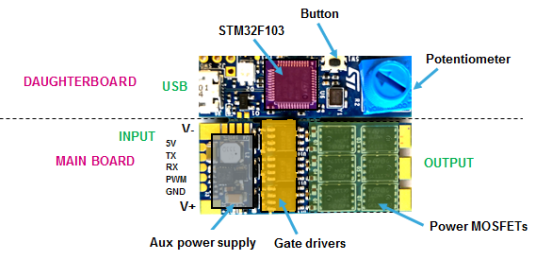
\includegraphics[width=\textwidth]{References/B-G431B-ESC1 top view.png}}
				\caption{B-G431B-ESC1 Top View}
			\end{figure}
			\begin{figure}[H]
				\centerline{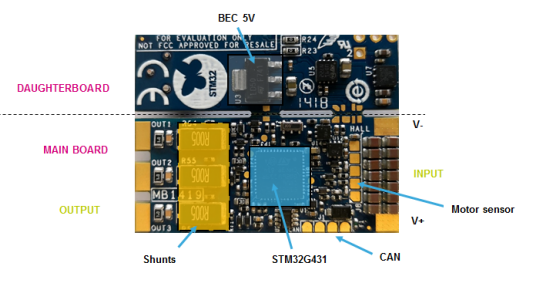
\includegraphics[width=\textwidth]{References/B-G431B-ESC1 bottom view.png}}
				\caption{B-G431B-ESC1 Bottom View}
			\end{figure}
		\FloatBarrier \subsection{ElectroCraft RPX32-090V24-110-R}
			\begin{itemize}
                \item \href{https://www.electrocraft.com/products/bldc/RPX32/}{Product Page}
                \item \href{../RPX32-DataSheet-US.pdf}{RPX32 Data Sheet}
            \end{itemize}
			\begin{itemize}
				\item \textbf{RPX32} - RapidPower Xtreme 32mm
				\item \textbf{090V24} - 90 mNm torque, 24 V
				\item \textbf{110} - Rear Shaft, Flat Front Shaft, Flying Leads
				\item \textbf{R} - 1024 Line Diff Encoder
			\end{itemize}
		
	\FloatBarrier \section{Needed Software}
        Below is a list of necessary software for this project. In parenthesis is the version I have.
        \begin{itemize}
            \item IAR Embedded Workbench for Arm (9.50.2)
            \item ST Motor Control SDK (5.4.8)
            \item ST Motor Control SDK (6.2.1)
            \item STM32CubeMX (6.11.0)
            \item Sentinel System Driver Installer (7.6.1)
            \item Git (2.45.0)
        \end{itemize}
        If links below do not work, a list of included software will be included in the git repository \texttt{https://github.com/austin-green-ltg/STM32G431-Downloads}.  You will need to unzip these files in their corresponding directory. This is included in a separate repository because of the file size being so large. Learn how to use git below.
		\FloatBarrier \subsection{IAR Embedded Workbench for Arm}
            \href{https://www.iar.com/products/architectures/arm/iar-embedded-workbench-for-arm/}{Link}
			\FloatBarrier \subsubsection{Description}
                IDE and compiler that is DAL certified. Will need license (can use dongle and activate license in license manager).
			\FloatBarrier \subsubsection{Installation}
                Double click installer and go though steps. Only a few changes are needed in the EWARM installer
                \begin{enumerate}
                    \item On the USB Driver installation page, you only need the \emph{ST-LINK Debug probe drivers}. Also, scroll down and select \emph{Dongle drivers} option.
                \end{enumerate}
                \emph{IMPORTANT:} remove dongle from system before continuing with dongle driver install.
                \begin{figure}[H]
                    \centerline{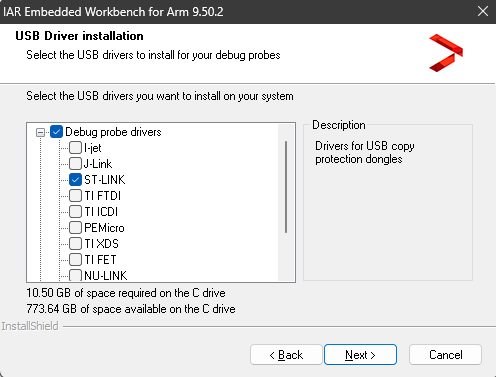
\includegraphics[width=\textwidth]{References/Debug probe drivers.png}}
                \end{figure}
                \begin{figure}[H]
                    \centerline{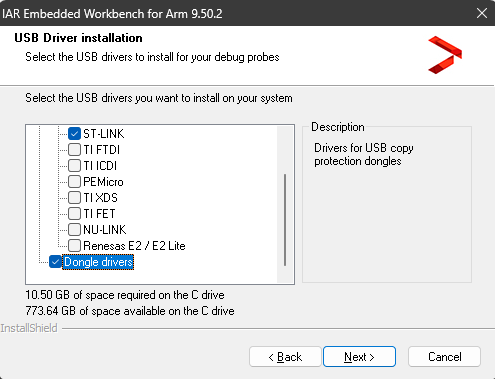
\includegraphics[width=\textwidth]{References/Dongle drivers.png}}
                \end{figure}
			\FloatBarrier \subsubsection{Configuration}
                After installation, there will be a piece of software on your computer called \emph{IAR License Manager for ARM}. You will need to go into this software and go to License\texttt{->}Activate License...\texttt{->}Online activation and insert any license keys associated with any dongles you plan to use. 
		\FloatBarrier \subsection{ST Motor Control SDK}
            \href{https://www.st.com/en/embedded-software/x-cube-mcsdk.html}{Link}
			\FloatBarrier \subsubsection{Description} 
                Install both versions of this software (V5.4.8 and Latest(6.2.1 for me)). The ST Motor Control SDK includes three pieces of software, the MotorControl Workbench, the Motor Pilot, and the Motor Profiler. The reason that two versions of ST Motor Control SDK are included is that the profiler included in 6+ is more difficult to use so will be saved for later. \emph{NOTE:} MotorControl Workbench 5.4.8 will be installed on your system, but it is unused. Only The Motor Profiler 6.2.1 is used from this package.
			\FloatBarrier \subsubsection{Installation}
                Double click installer and go though steps. It is recommended that you install this in the default location. I have found ST software has a hard time finding the other ST software if you move it.
			\FloatBarrier \subsubsection{Configuration}
                No configuration necessary for this software.
		\FloatBarrier \subsection{STM32CubeMX}
            \href{https://www.st.com/en/development-tools/stm32cubemx.html}{Link}
			\FloatBarrier \subsubsection{Description} 
                This is where you can configure pinouts and download software for the board and install firmware to the board. You will not spend a ton of time in this as most of the configuration will be in the MotorControl Workbench.
			\FloatBarrier \subsubsection{Installation}
                Double click installer and go though steps. It is recommended that you install this in the default location. I have found ST software has a hard time finding the other ST software if you move it.
			\FloatBarrier \subsubsection{Configuration}
                While it is not strictly necessary, it is recommended that before you continue, you launch the STM32CubeMX software. On the right side of the screen, there is an \emph{INSTALL/REMOVE} button on below the \emph{Install or remove embedded software packages}. Click on this and scroll down to your CPU series (STM32G4 in this case) and install the latest pack and any subversions of it (currently 1.5.0-1.5.2). If you are having trouble, future steps will allow for the automatic installation of any necessary packages.
                \begin{figure}[H]
                    \centerline{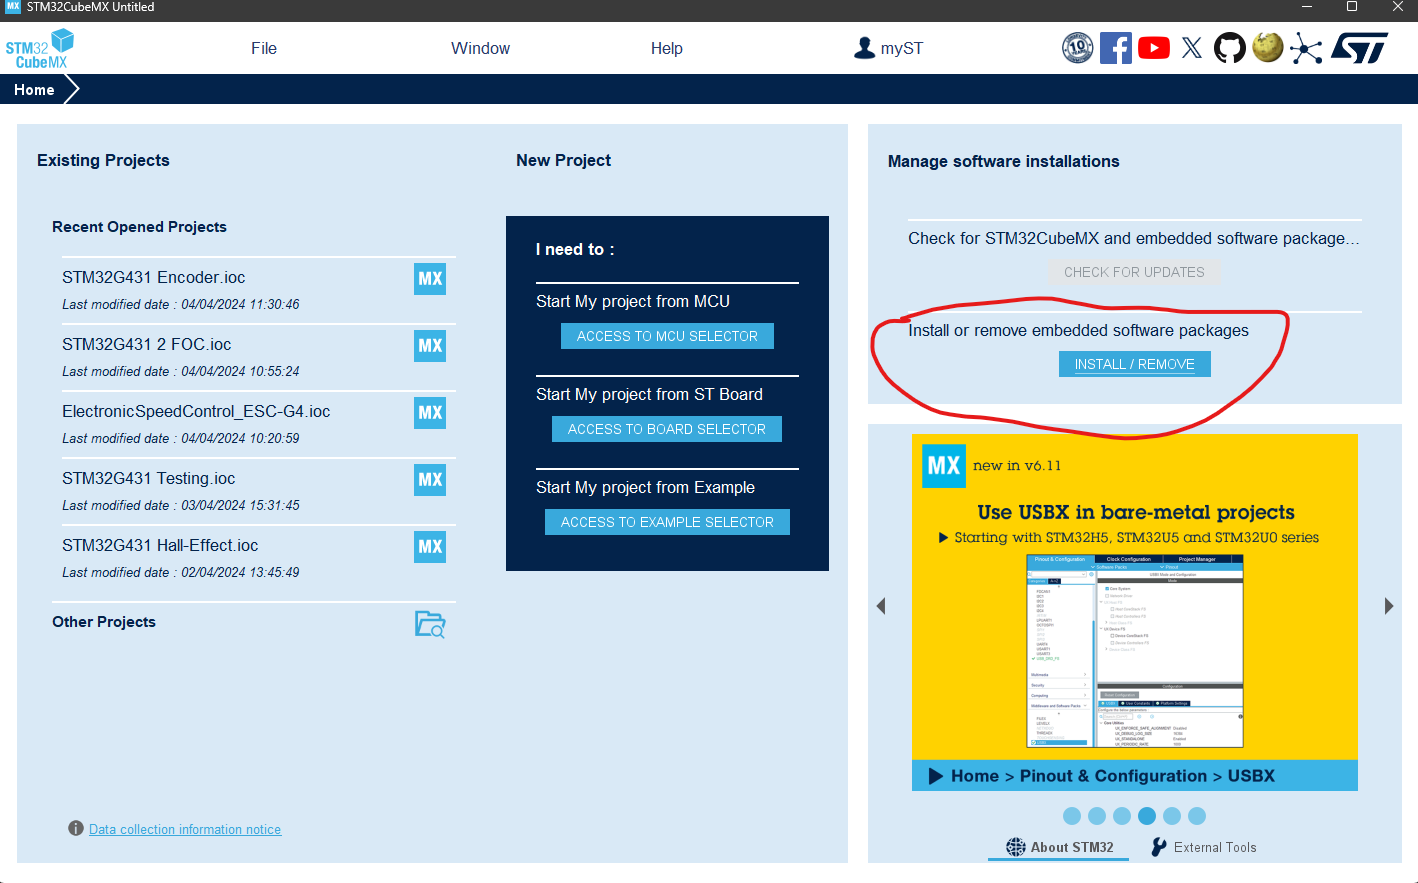
\includegraphics[width=\textwidth]{References/ST32CubeMX.png}}
                    \caption{ST32CubeMX Launch Page}
                \end{figure}
                \begin{figure}[H]
                    \centerline{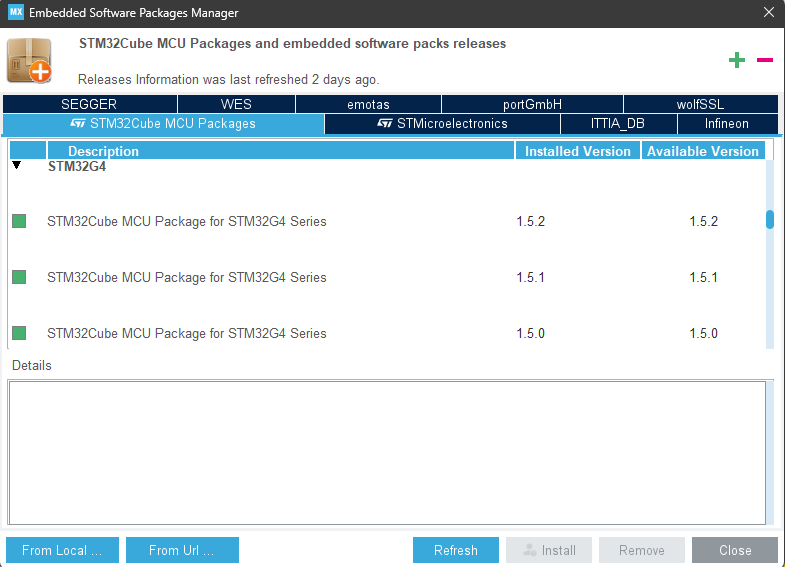
\includegraphics[width=\textwidth]{References/Pack Installer.png}}
                    \caption{Pack Installer}
                \end{figure}
		\FloatBarrier \subsection{Sentinel System Driver Installer}
            \href{https://supportportal.thalesgroup.com/csm?id=kb_article_view&sys_kb_id=e88691ba37edcb08cc47261953990e80&sysparm_article=KB0016514}{Link}
			\FloatBarrier \subsubsection{Description} 
                IAR License Dongle driver.
			\FloatBarrier \subsubsection{Installation}
                Double click installer and go though steps.
			\FloatBarrier \subsubsection{Configuration}
                No configuration necessary for this driver.
		\FloatBarrier \subsection{Git}
            \href{https://git-scm.com/downloads}{Link}
			\FloatBarrier \subsubsection{Description} 
                Version control software
			\FloatBarrier \subsubsection{Installation}
                Double click installer and go though steps.
			\FloatBarrier \subsubsection{Configuration}
				\paragraph{Pulling a Repo}
                    After downloading, navigate to a folder you wish to place this project in and right click in the folder. Select \emph{Open Git Bash here}. This will pop up a window. In this window type the command \\ 
                    \texttt{git clone https://github.com/austin-green-ltg/STM32G431-MotorControlWorkbench.git} \\ 
                    This will clone the project to your local directory.
				\paragraph{Checking out a branch}
                    In that same window, type cd STM32G431-MotorControlWorkbench. CD stand for change directory and will bring you into the STM32G431-MotorControlWorkbench directory, similarly had you double clicked on the folder. In each section will be two pieces of git-related information:
                    \begin{enumerate}
                        \item \textbf{The Branch} - The name of the location where the code files for that section lies. To get the branch, open \emph{Git Bash} and type \texttt{git checkout <branch name>}.
                        \item \textbf{The Commit} - The specific files associated with that subsection. To get the commit, open \emph{Git Bash} and type \texttt{git checkout <commit name>}.
                    \end{enumerate}
	\FloatBarrier \section{Wiring Motor}
        There are two main parts to wiring up the motor.
		\FloatBarrier \subsection{Wiring Up Motor Lines}
            There are five wires that need to be soldered to the board in order to get the motor operational. The first two are the V+ and V- lines for power and ground to connect to a power supply and the final three are the Motor wires. You can see their location here: 
			\begin{figure}[H]
				\centerline{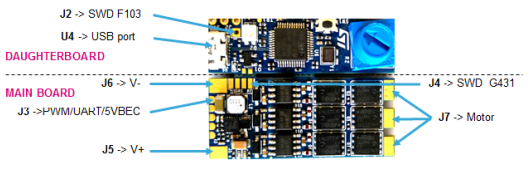
\includegraphics[width=\textwidth]{References/Power Wiring.png}}
				\caption{Pad location for V+ (J5), V- (J6), and Motor (J7)}
			\end{figure}
            You should use 22 gage wires as listed in the hardware section above to wire up power and ground. These are the same gage used by the motor. \\ 
            The motor wires can be seen here:
			\begin{figure}[H]
				\centerline{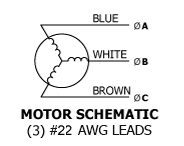
\includegraphics[width=\textwidth]{References/Motor Wiring.png}}
				\caption{RPX32 Motor Wire Colors}
			\end{figure}
            I don't believe that which wires connect to which board outputs matter, but I wired up $\theta A$ to OUT1 (silk screened on the board), $\theta B$ to OUT2, and $\theta C$ to OUT3.
			\begin{figure}[H]
				\centerline{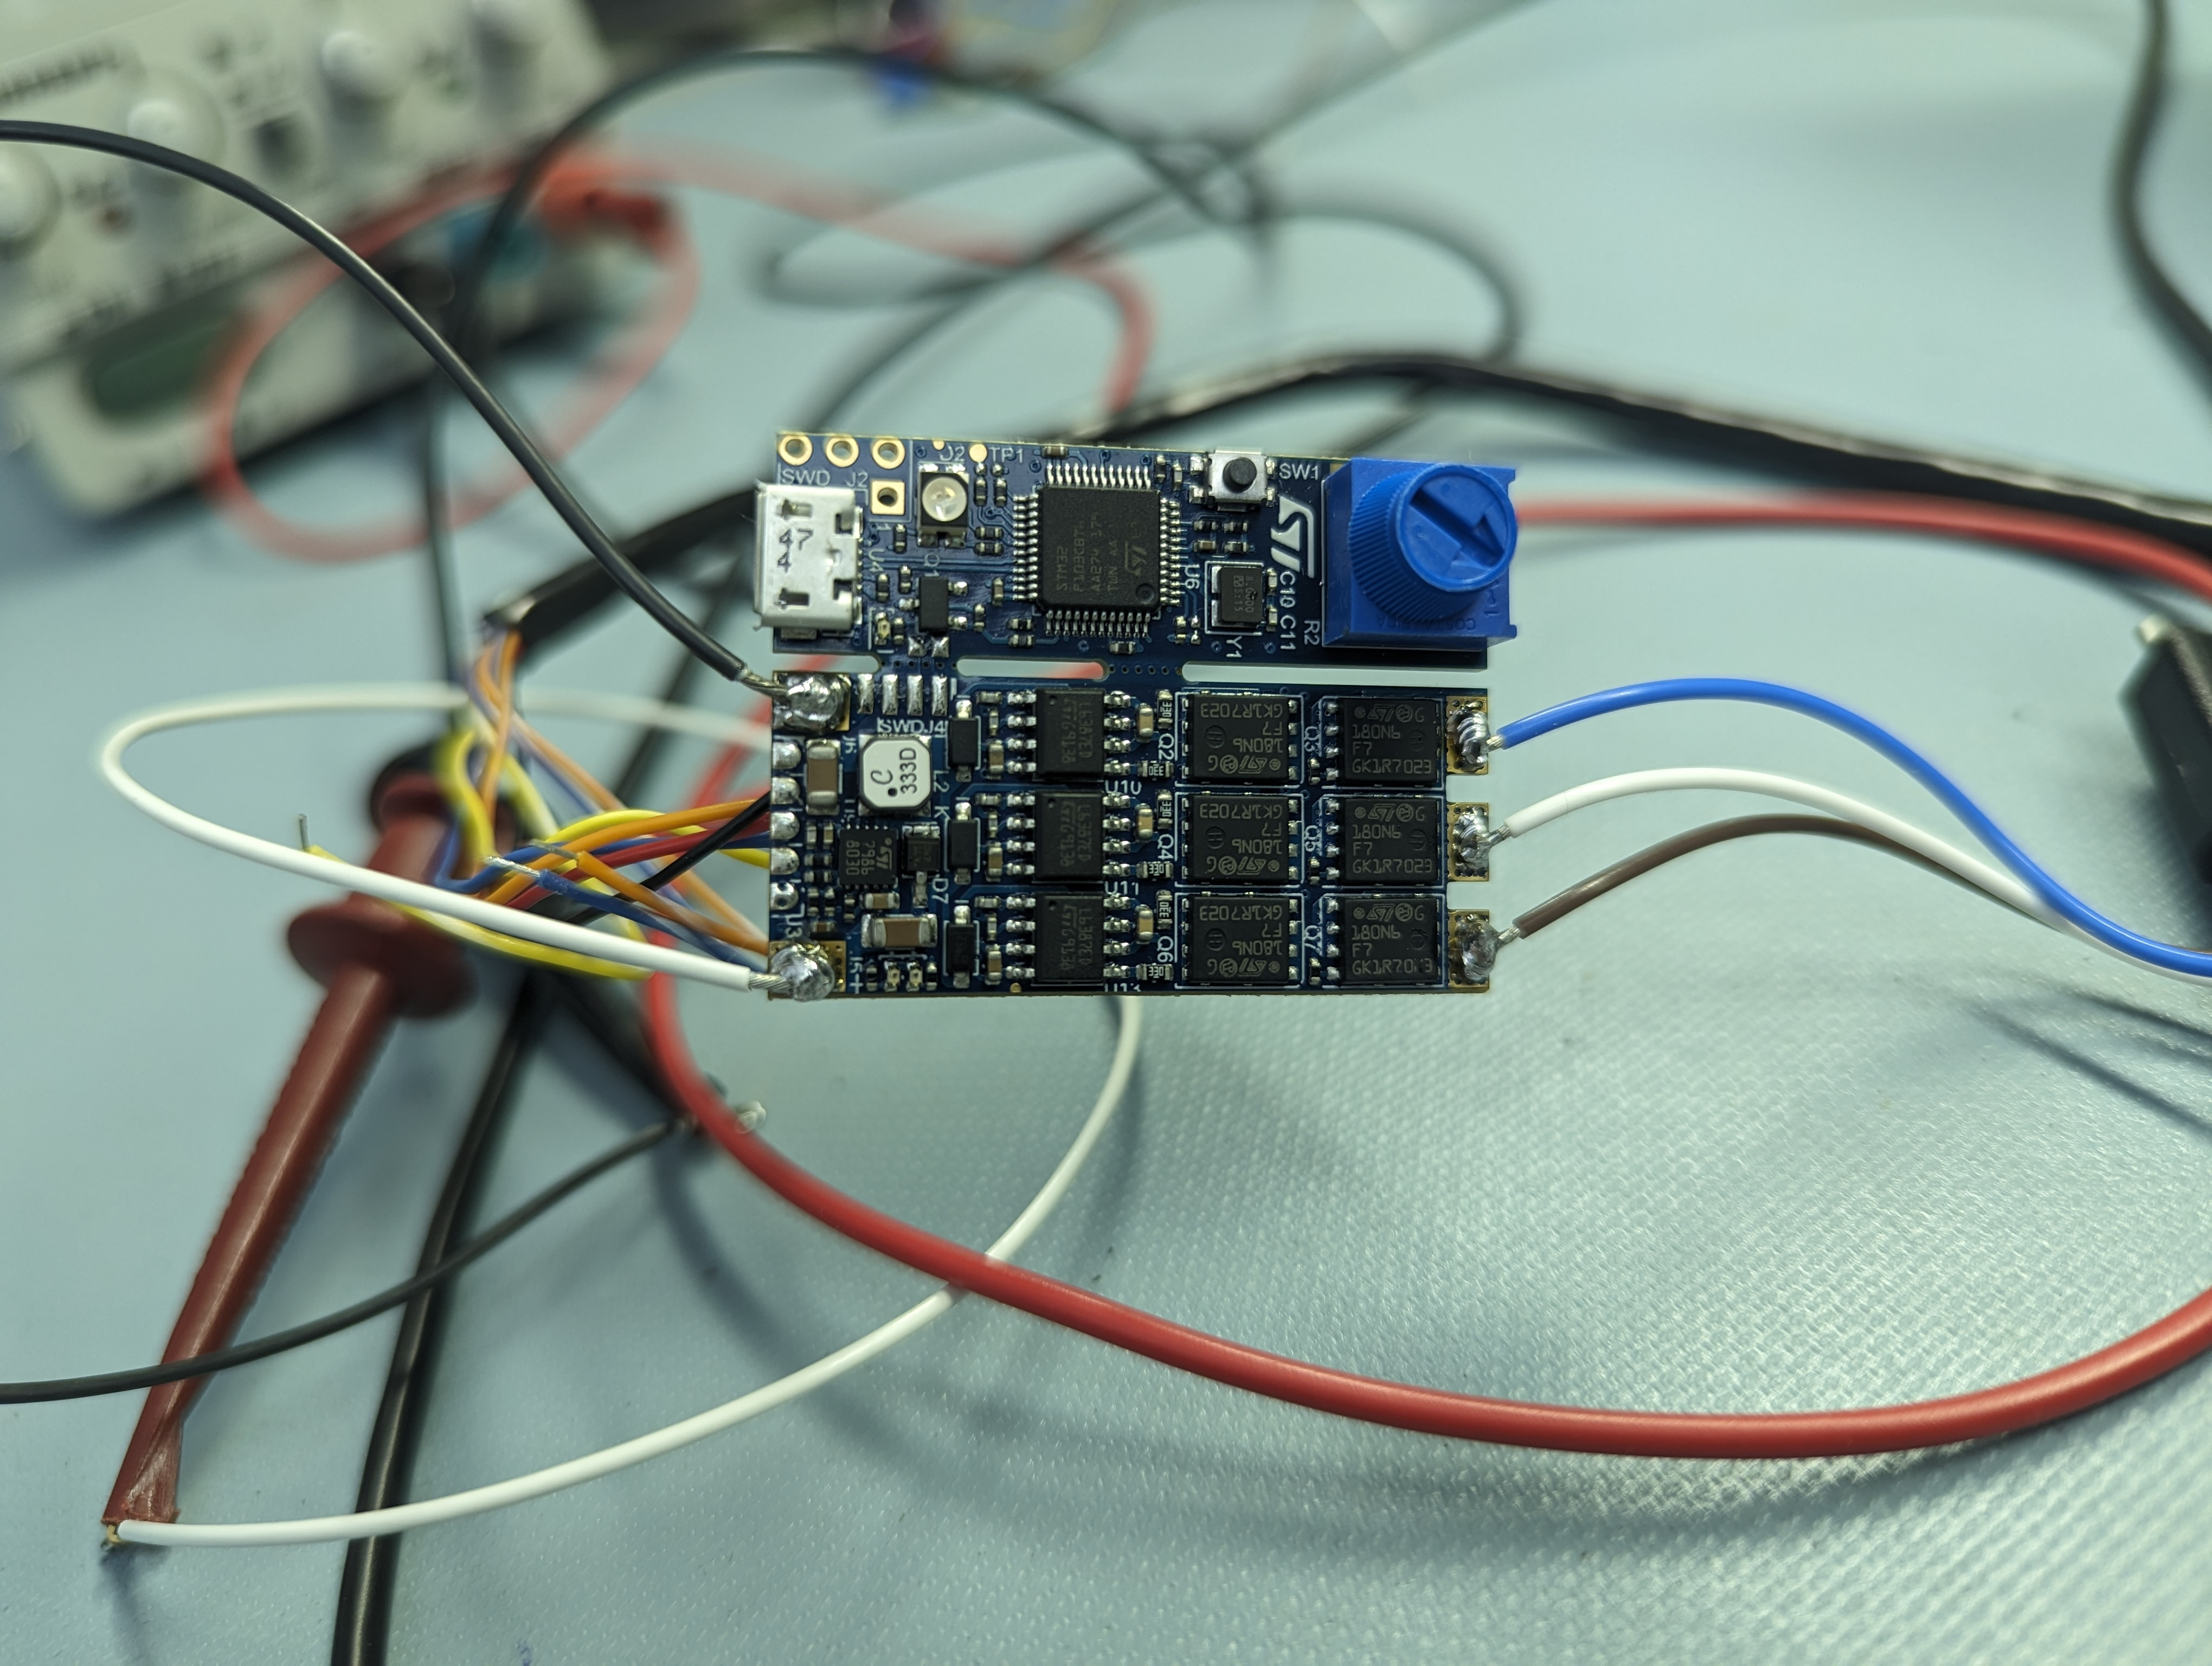
\includegraphics[width=\textwidth]{References/Motor Wiring Board Picture.jpg}}
				\caption{Motor Wiring Board Picture}
			\end{figure}
	\FloatBarrier \section{Profiling Motor}
		Manually inputting parameters of the motor is inexact. To get around this, we can use the profiler. Version 5.4.8 is less complicated but doesn't work as well with the FOC algorithm; Version 6.2.1 is more complicated but more precise.
		\FloatBarrier \subsection{MotorControl Workbench V5.4.8}
            \begin{itemize}
                \item Open \emph{Motor Profiler 5.4.8}.
                \begin{figure}[H]
                    \centerline{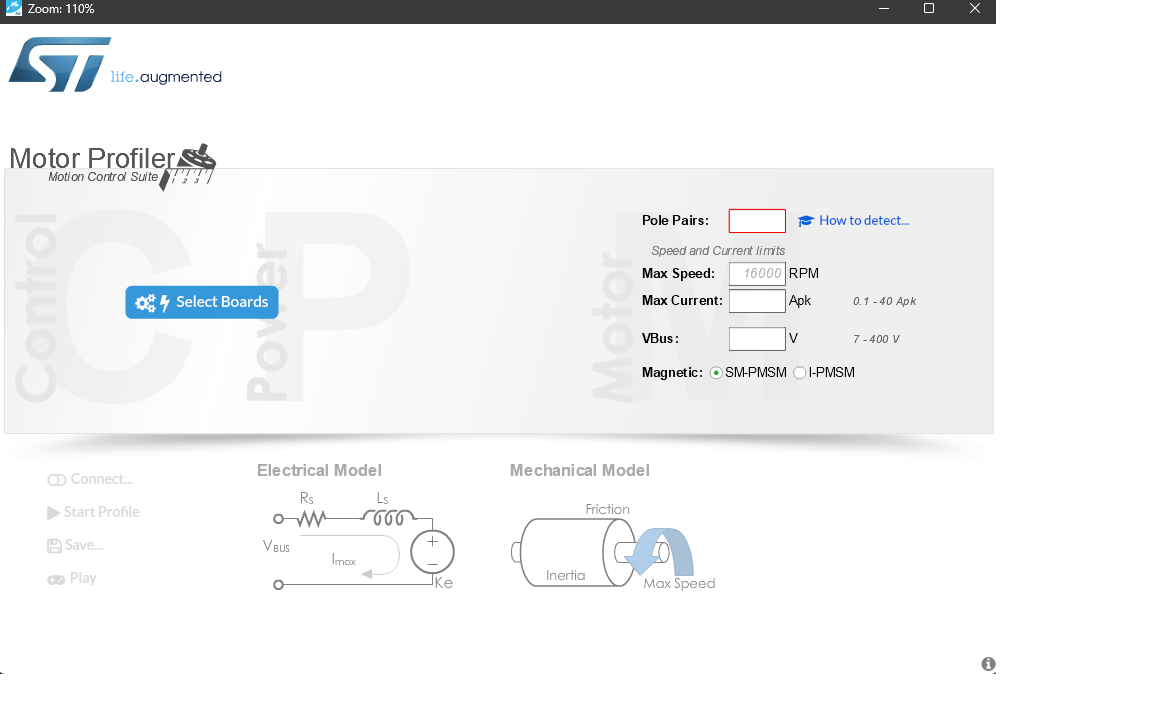
\includegraphics[width=\textwidth]{References/Motor Profiler.png}}
                    \caption{Motor Profiler 5.4.8}
                \end{figure}
                \item Click on \emph{Select Boards} in the middle of the screen. Our board is \emph{B-G431B-ESC1}.
                    \begin{figure}[H]
                        \centerline{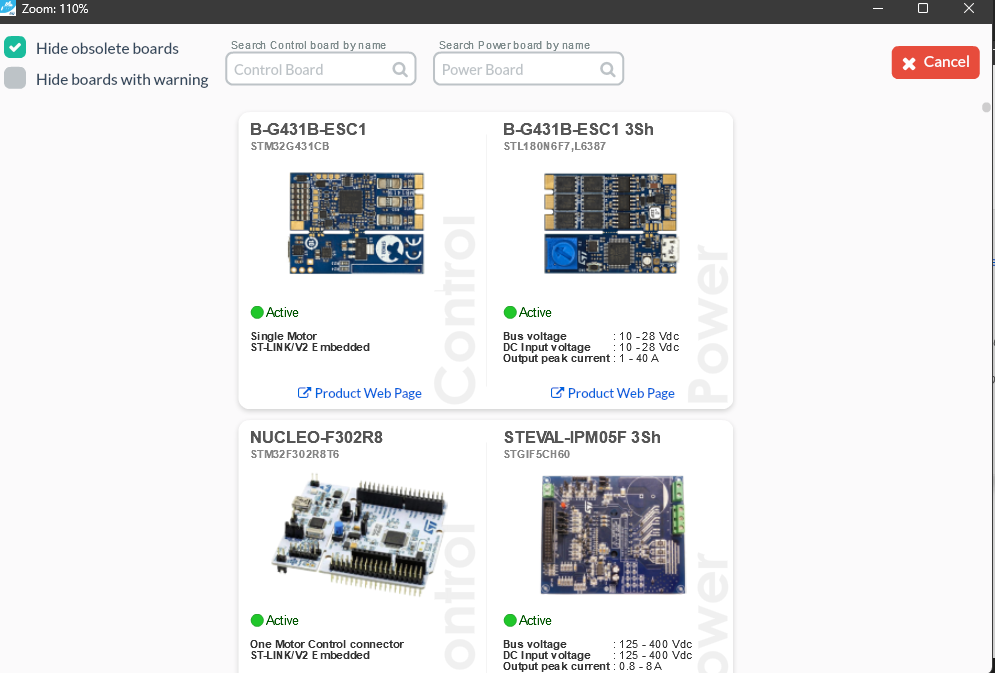
\includegraphics[width=\textwidth]{References/Motor Profiler Select Board.png}}
                        \caption{Select Board}
                    \end{figure}
                \item Fill out the information on the right side of the screen. This can be found on the RPX32 Data Sheet as well as the website
                    \begin{itemize}
                        \item Pole Pairs = 4
                        \item Max Speed = 9600 RPM
                        \item Max Current = 4 Apk
                        \item VBus = 24V
                        \item Magnetic = SM-PMSM
                    \end{itemize}
                    \begin{figure}[H]
                        \centerline{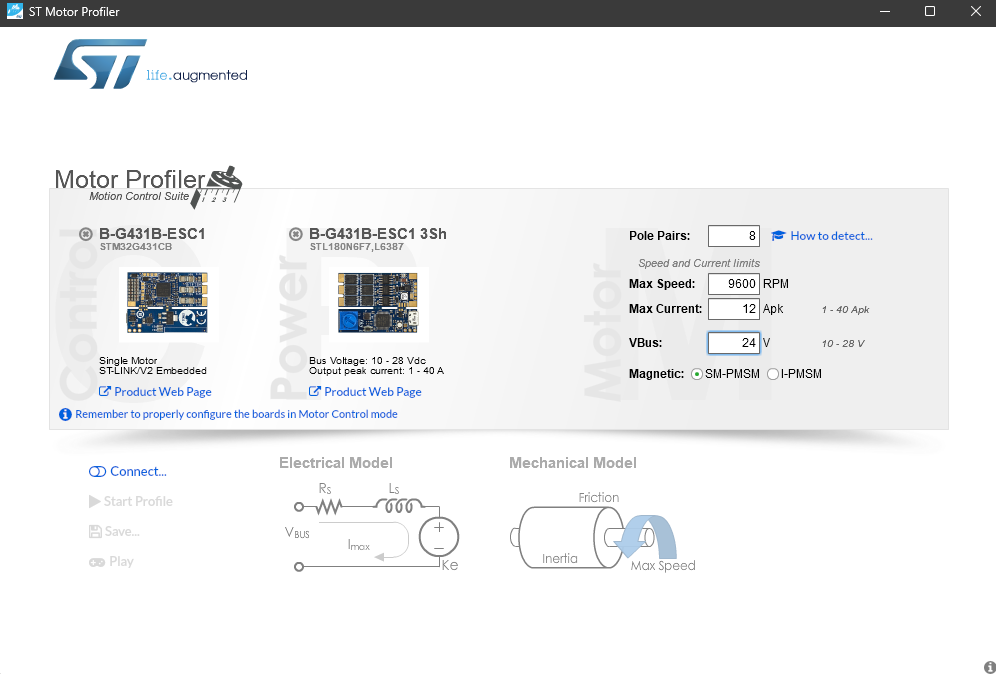
\includegraphics[width=\textwidth]{References/Motor Profiler Parameters.png}}
                        \caption{Motor Profiler Filled Parameters}
                    \end{figure}
                \item Connect microcontroller via USB cable to your computer.
                \item Click on \emph{Connect...} on the bottom. It may tell you that a Firmware upgrade is required, if so, select \emph{Upgrade Firmware}
                \item Connect microcontroller to power supply set to 24V via soldered V+ and V- wires. Ensure that the motor is able to draw at least 4 amps.
                \item Select \emph{Start Profile}, this may take a while. After profile is done, ensure that you select \emph{Save...} and name it something recognizable i.e. ElectroCraft RPX32.
            \end{itemize}
		\FloatBarrier \subsection{MotorControl Workbench V6+}
            This is more time consuming but worth it when precise control matters. 
            \begin{itemize}
                \item Open \emph{MotorControl Workbench V6+} and click on \emph{Tools} - \emph{Motor Profiler}. Leave this alone for now.
                \item On the Motor Control WorkBench, select \emph{New project} in the top left.
                \item Give your project a name like "STM32G431 Motor Profiler"
                \item \emph{Num. Motors} is 1 Motor, \emph{Driving Algorithm} is \emph{FOC}, and \emph{Hardware Mode} is Inverter. Click Next at the bottom right.
                    \begin{figure}[H]
                        \centerline{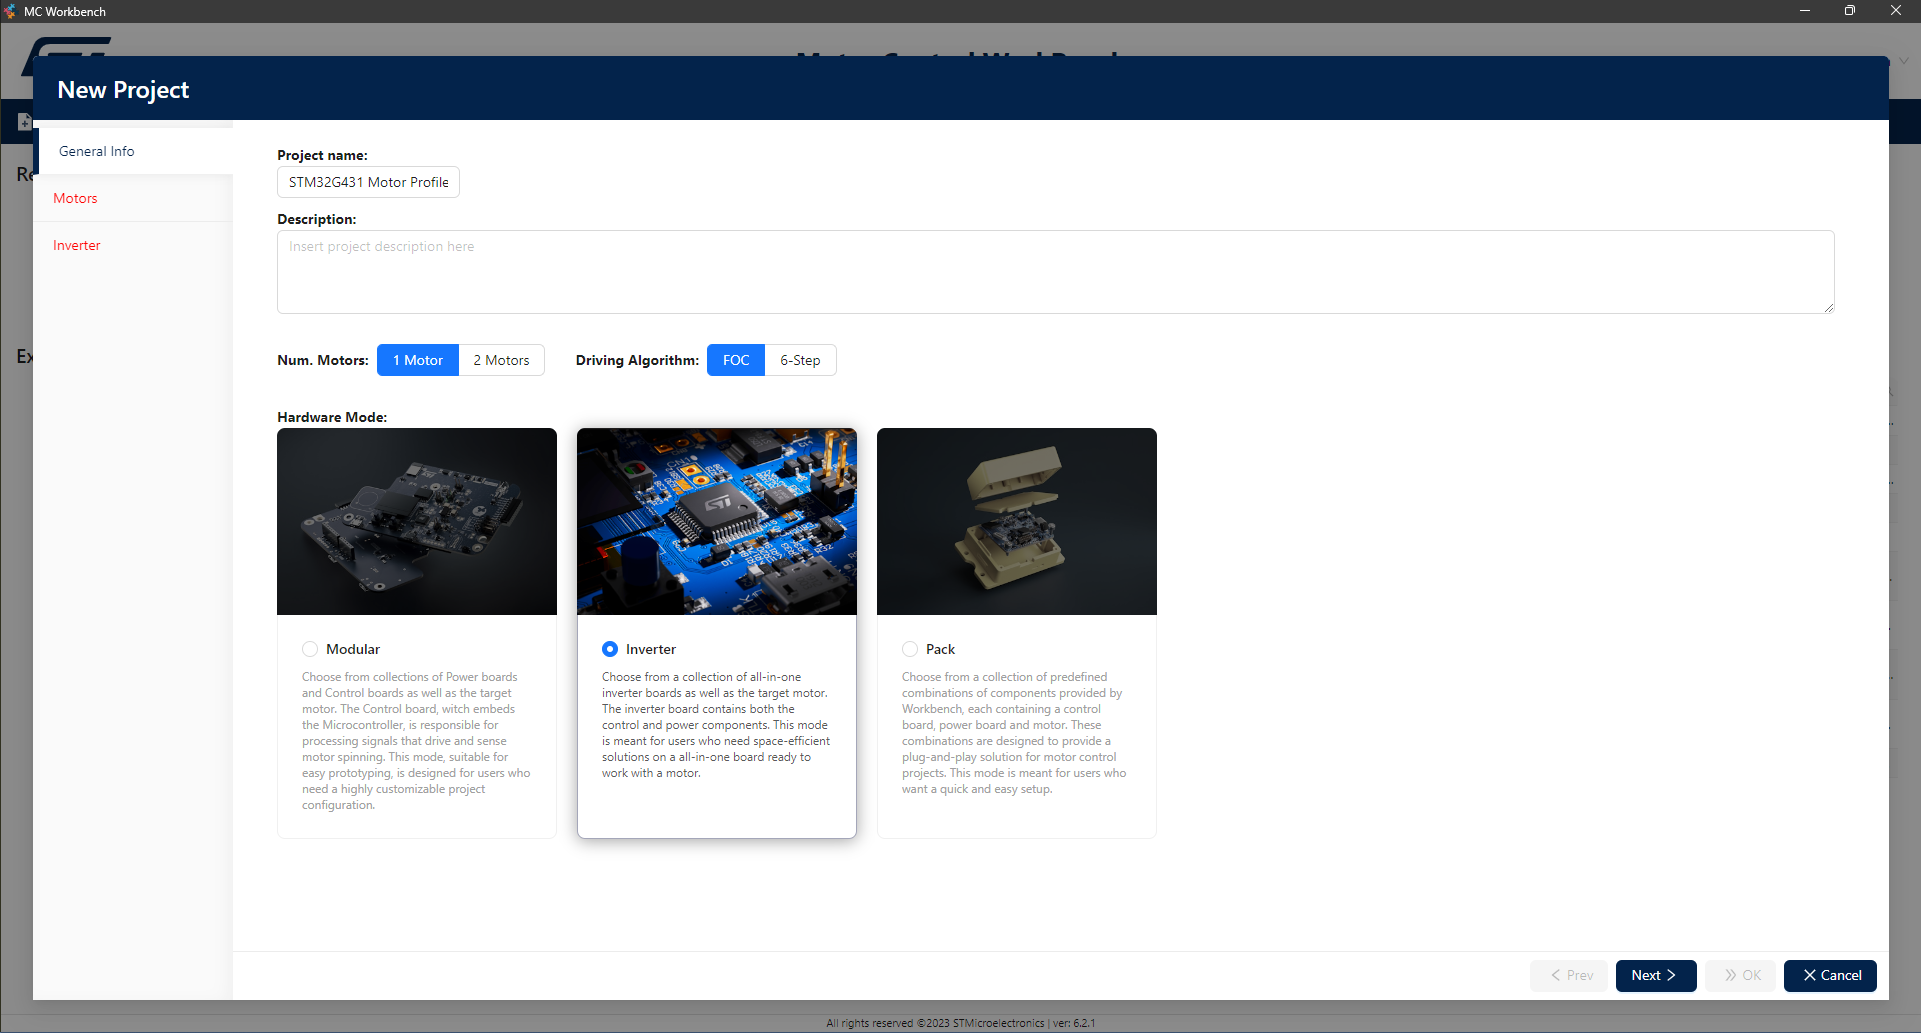
\includegraphics[width=\textwidth]{References/MCW Profiler New Project.png}}
                        \caption{MotorControl Workbench New Project}
                    \end{figure}
                \item Select the \emph{SM-PMSM 24V motor}.
                    \begin{figure}[H]
                        \centerline{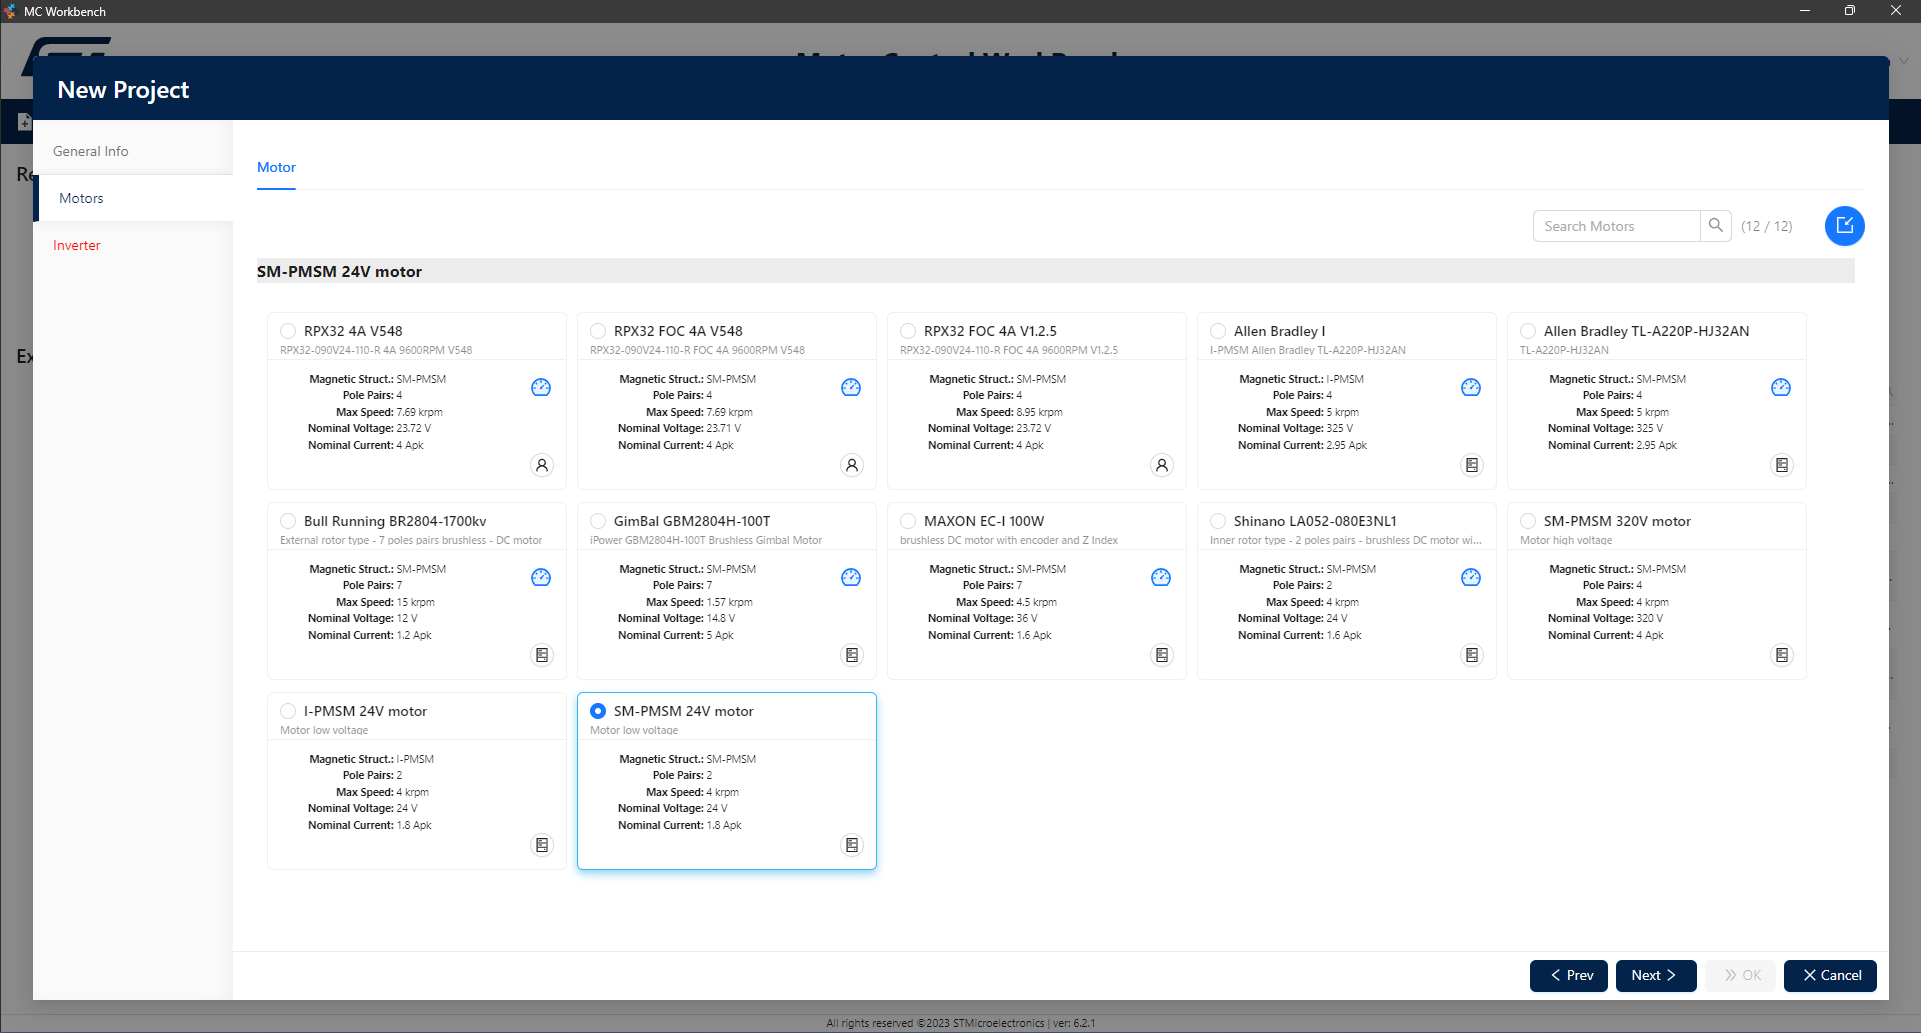
\includegraphics[width=\textwidth]{References/MCW Profiler Motor.png}}
                        \caption{MotorControl Workbench Motor}
                    \end{figure}
                \item Select B-G431B-ESC1 as your board. Click OK.
                \item This will bring you to the MotorControl Workbench Project screen.
                    \begin{figure}[H]
                        \centerline{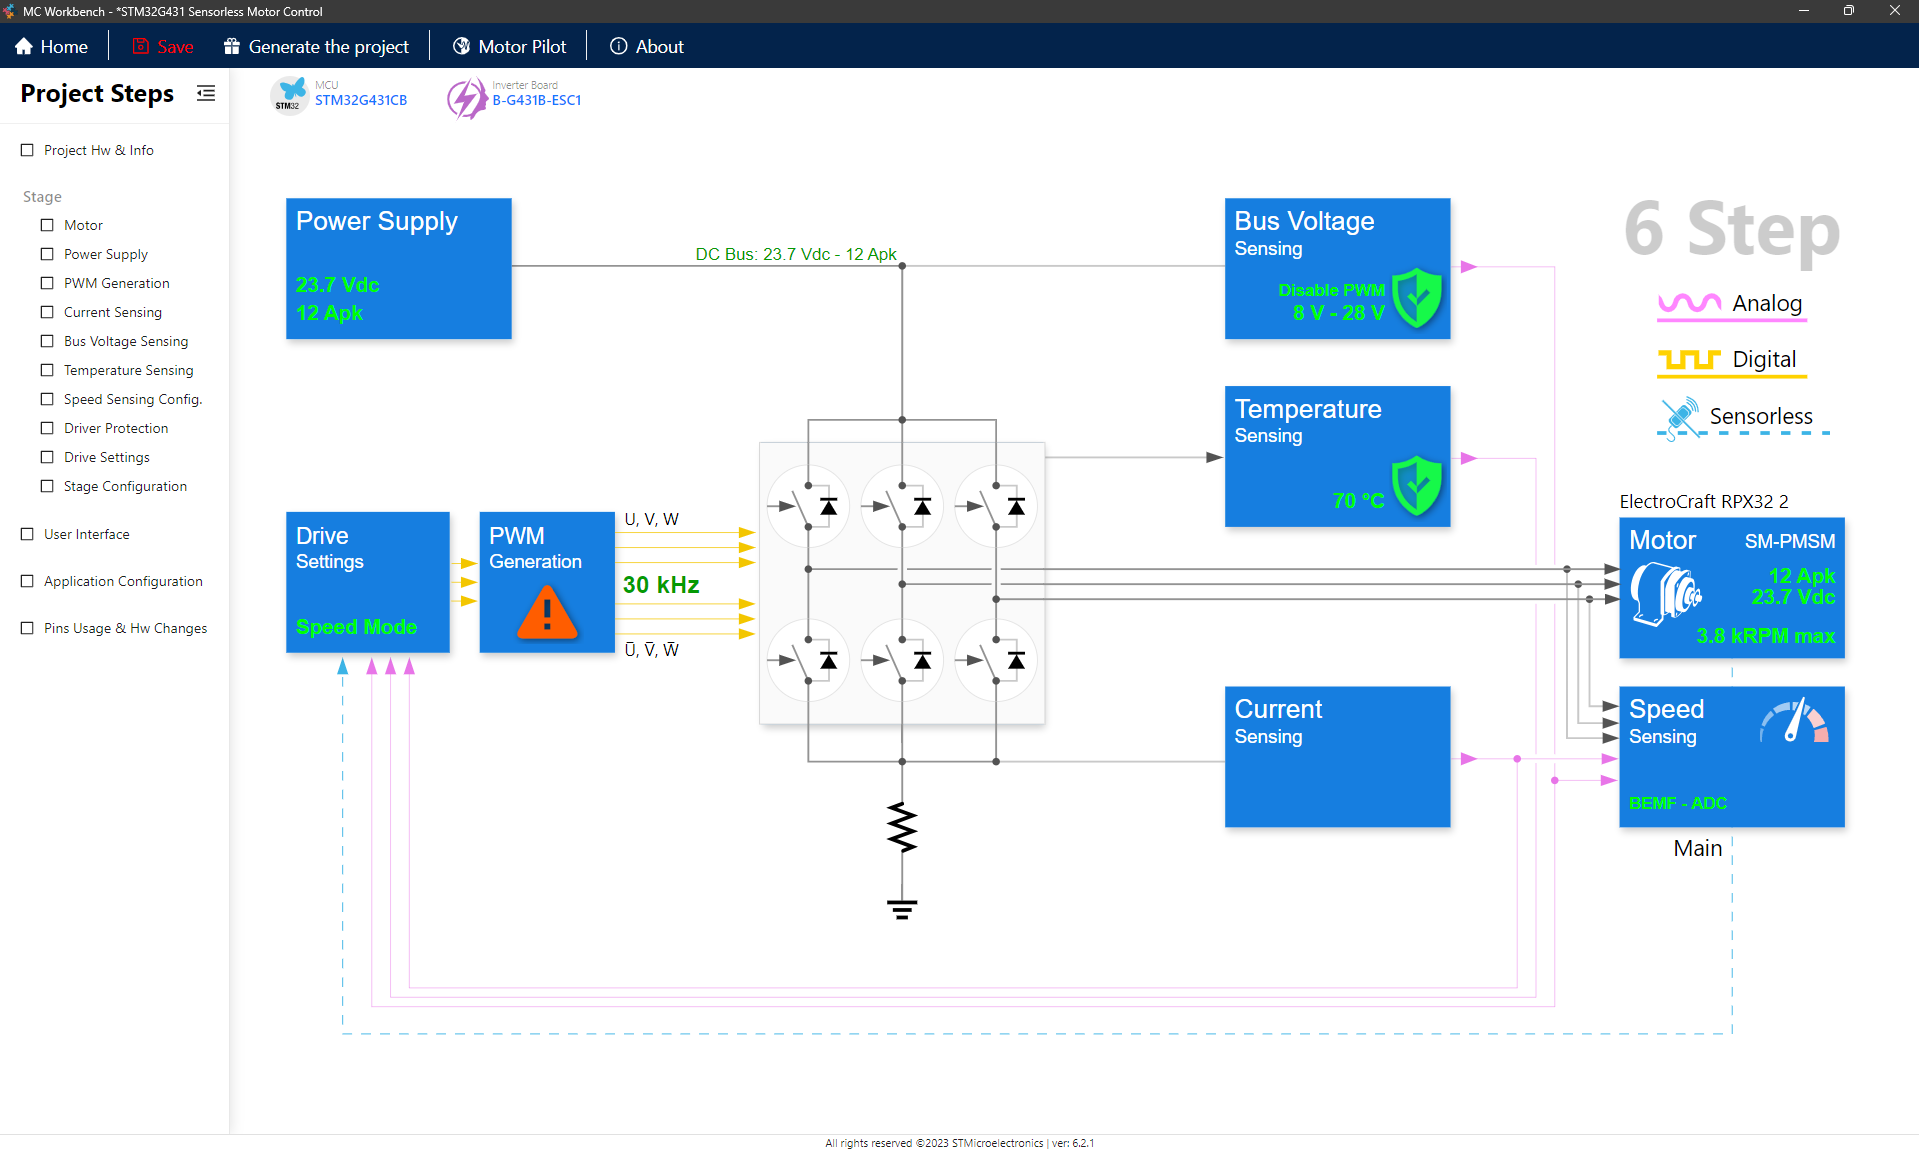
\includegraphics[width=\textwidth]{References/MCW Project Screen.png}}
                        \caption{MotorControl Workbench Project Screen}
                    \end{figure}
                \item From here, either click on \emph{Motor} on the left hand side or click the motor on the right hand side. Set \emph{Pole Pairs} to 4 and \emph{Max current} to 4 Apk.
                    \begin{figure}[H]
                        \centerline{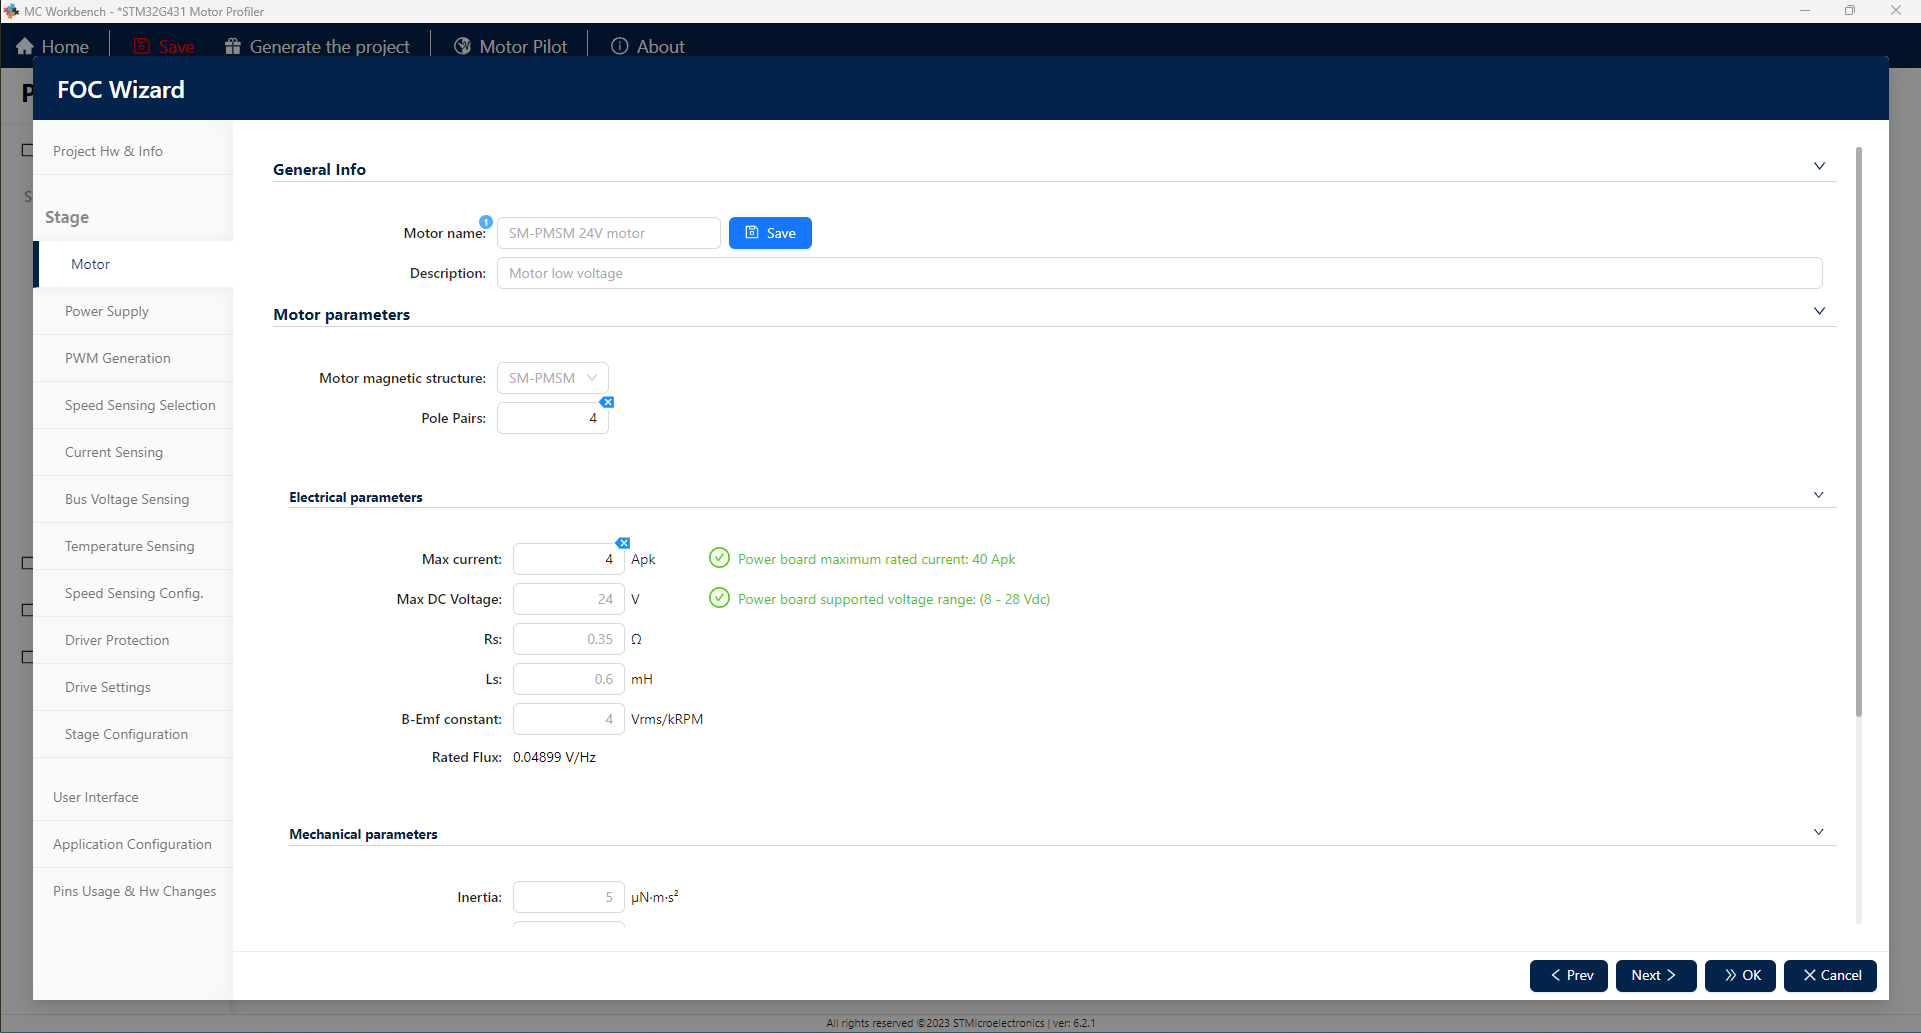
\includegraphics[width=\textwidth]{References/MCW Motor Profiling.png}}
                        \caption{MotorControl Workbench Motor Profiling Configuration}
                    \end{figure}
                \item Select \emph{Application Configuration} and select the \emph{Motor Profiler} check box and select \emph{OK} in the bottom right.
                    \begin{figure}[H]
                        \centerline{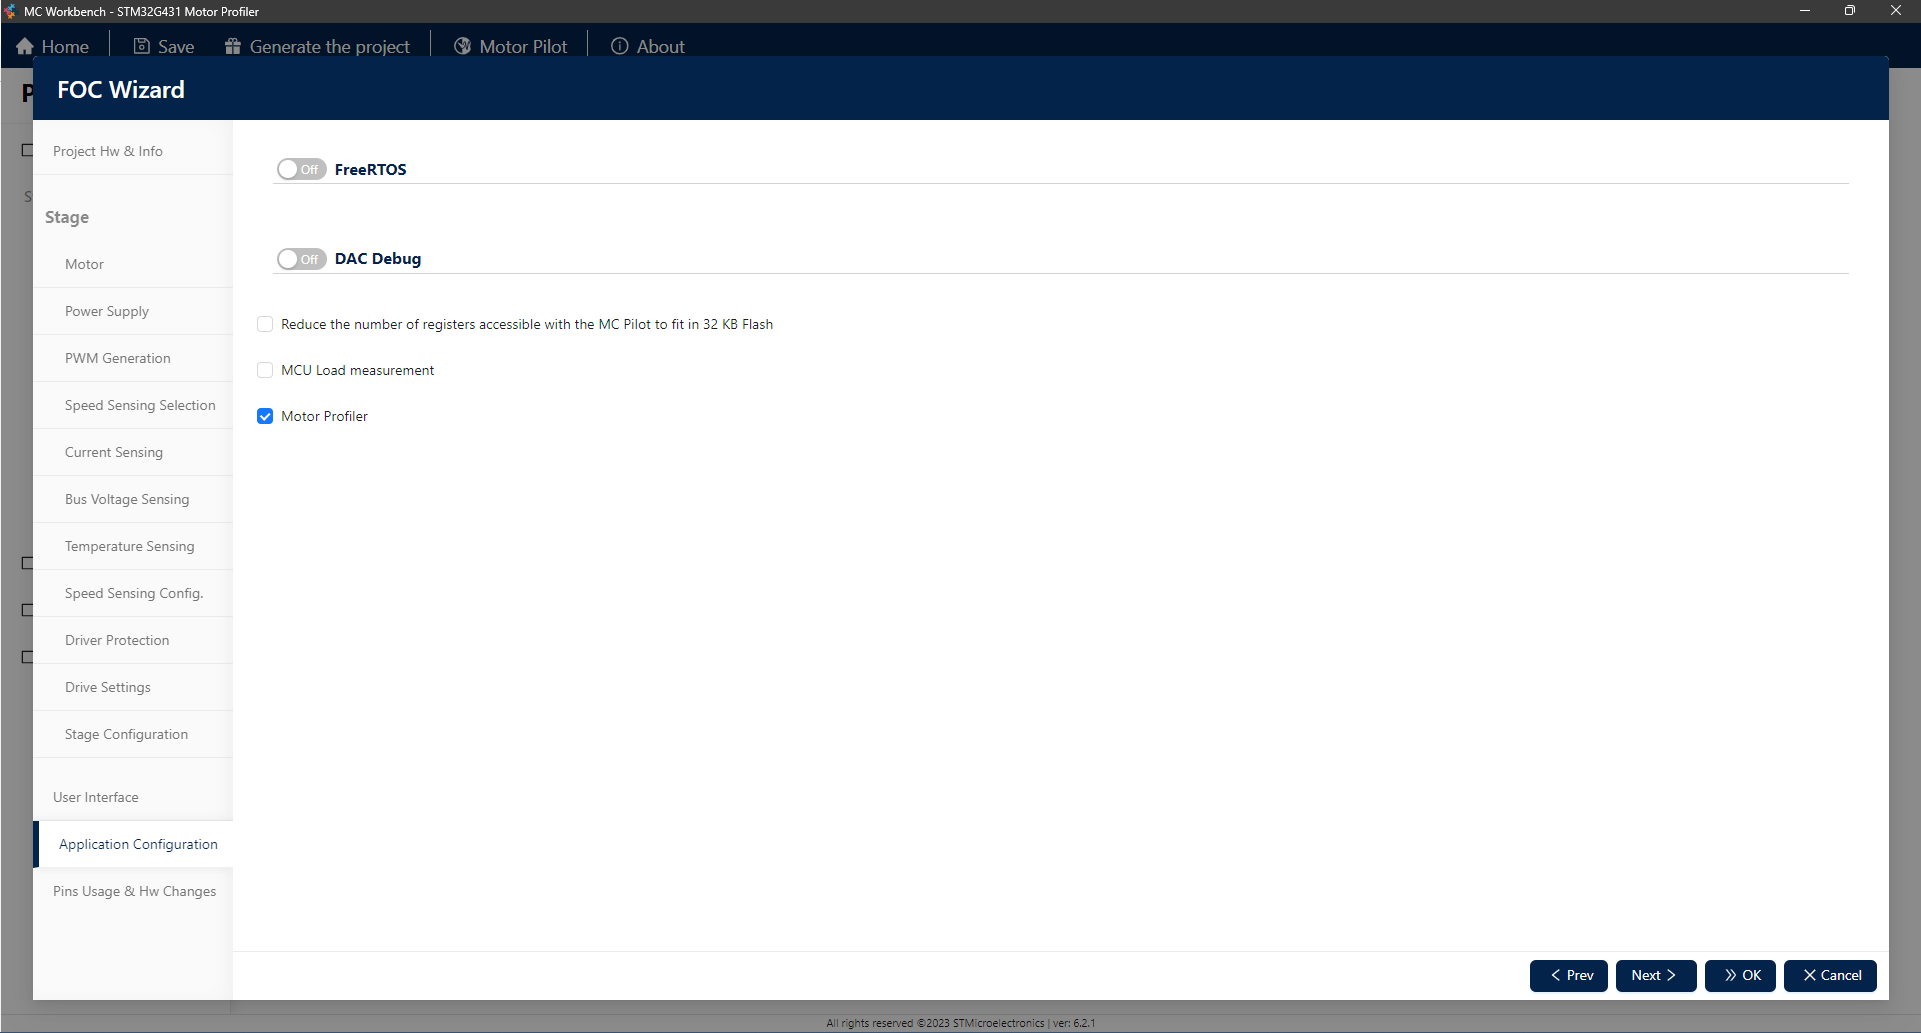
\includegraphics[width=\textwidth]{References/MCW Application Configuration Motor Profiler.png}}
                        \caption{MotorControl Workbench Application Configuration Motor Profiler}
                    \end{figure}
                \item Click \emph{Generate the project} at the top of the screen and save it.
                    \begin{figure}[H]
                        \centerline{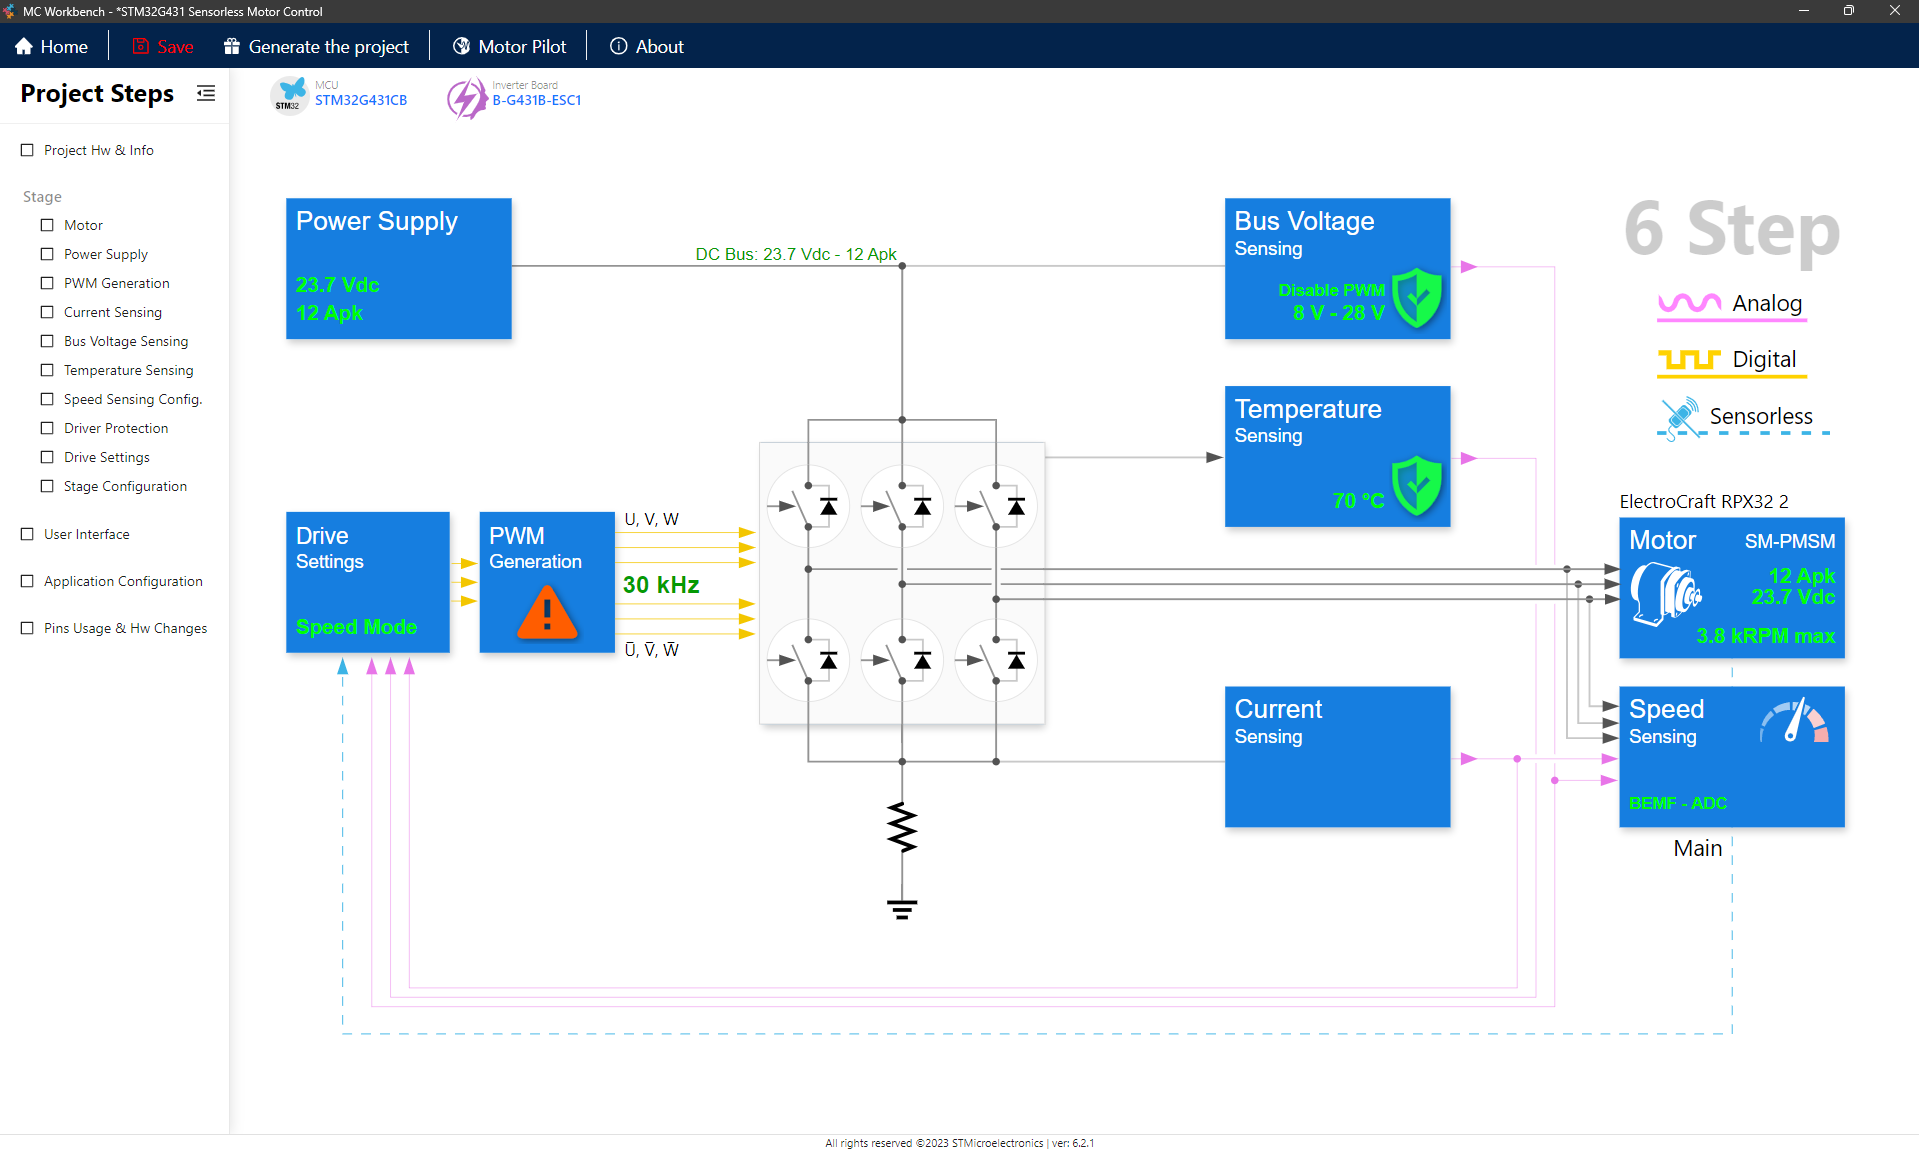
\includegraphics[width=\textwidth]{References/MCW Project Screen.png}}
                        \caption{MotorControl Workbench Project Screen}
                    \end{figure}
                \item Next the \emph{Project generation} screen will appear. Select the latest version of STM32CubeMX as your \emph{STM32CubeMX} version, select \emph{IAR EWARM V8} as your \emph{Target Toolchain}, and leave the recommended firmware under \emph{Firmware Package Version} and \emph{HAL - Hardware Abstraction Layer} as \emph{Drive Type}.
                    \begin{figure}[H]
                        \centerline{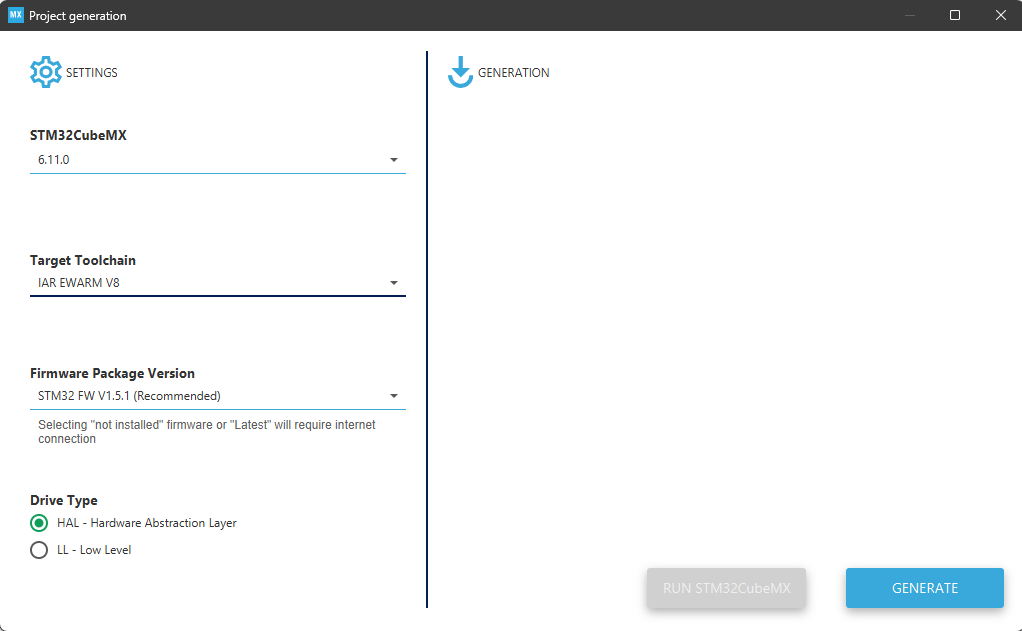
\includegraphics[width=\textwidth]{References/MCW Project Gen.png}}
                        \caption{MotorControl Workbench Project Generation Screen}
                    \end{figure}
                \item Select \emph{GENERATE}. It may ask you to install firmware, do so if prompted.
                \item Once completed, select \emph{RUN STM32CubeMX}.
                \item The only thing required to do in STM32CubeMX is click \emph{GENERATE CODE} in the top right and then \emph{Open Project} when completed.
                    \begin{figure}[H]
                        \centerline{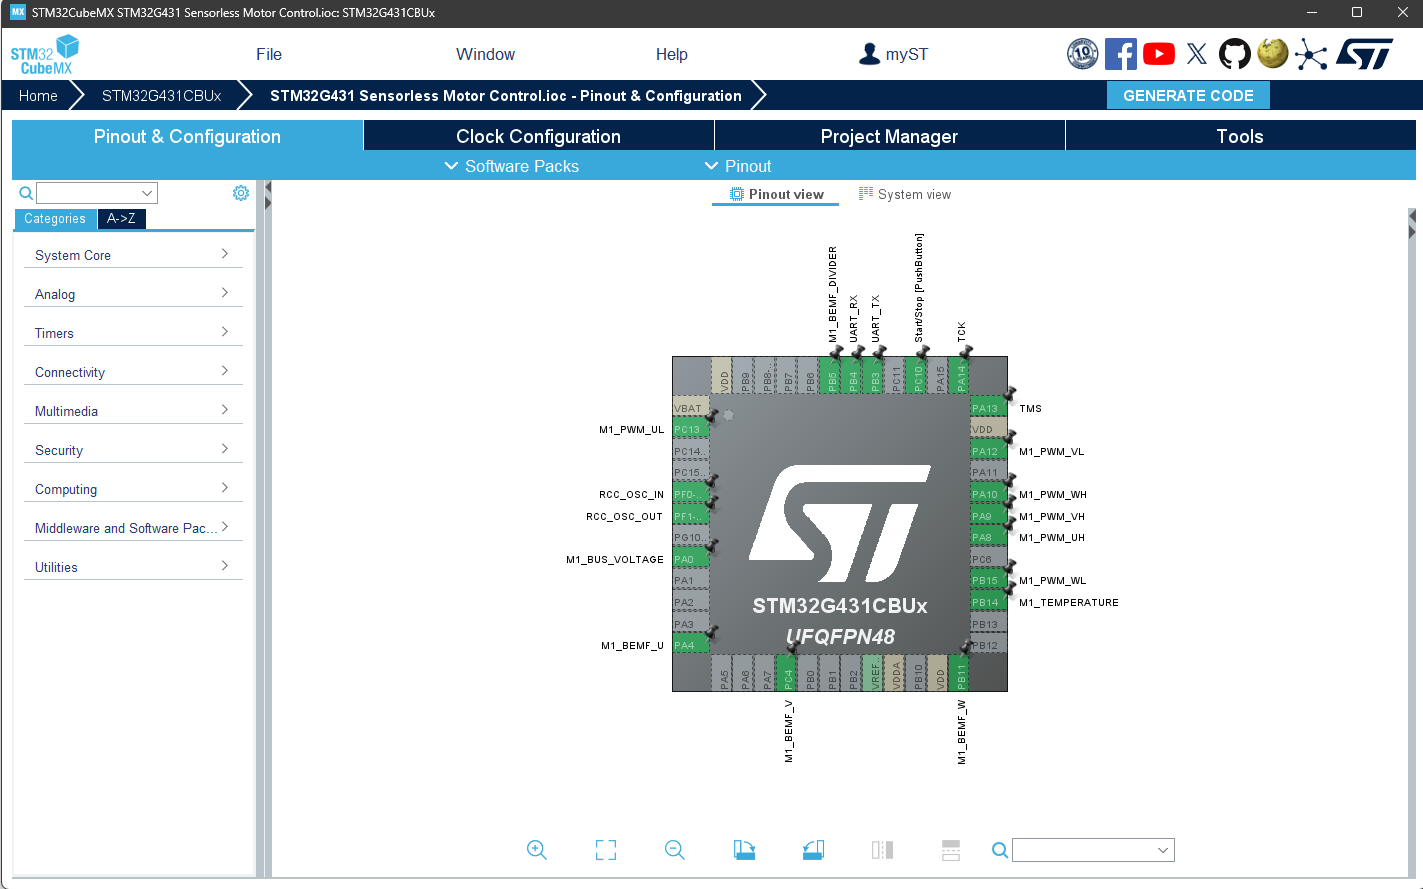
\includegraphics[width=\textwidth]{References/CubeMX.png}}
                        \caption{STM32CubeMX Project Screen}
                    \end{figure}
                \item A screen will pop up asking if you would like to upgrade the project to the latest IAR version. Do so. You can compile and download the project to the board in IAR using the green button with a white triangle. Once this completes, click run. 
                \item Now back to the profiler, select \emph{Connect} in the top left.
                \item Fill out the information on the right side of the screen. This can be found on the RPX32 Data Sheet as well as the website
                    \begin{itemize}
                        \item Pole Pairs = 4
                        \item Max Speed = 9600 RPM
                        \item Max Current = 4 Apk
                        \item VBus = 24V
                        \item Magnetic = SM-PMSM
                    \end{itemize}
                    \begin{figure}[H]
                        \centerline{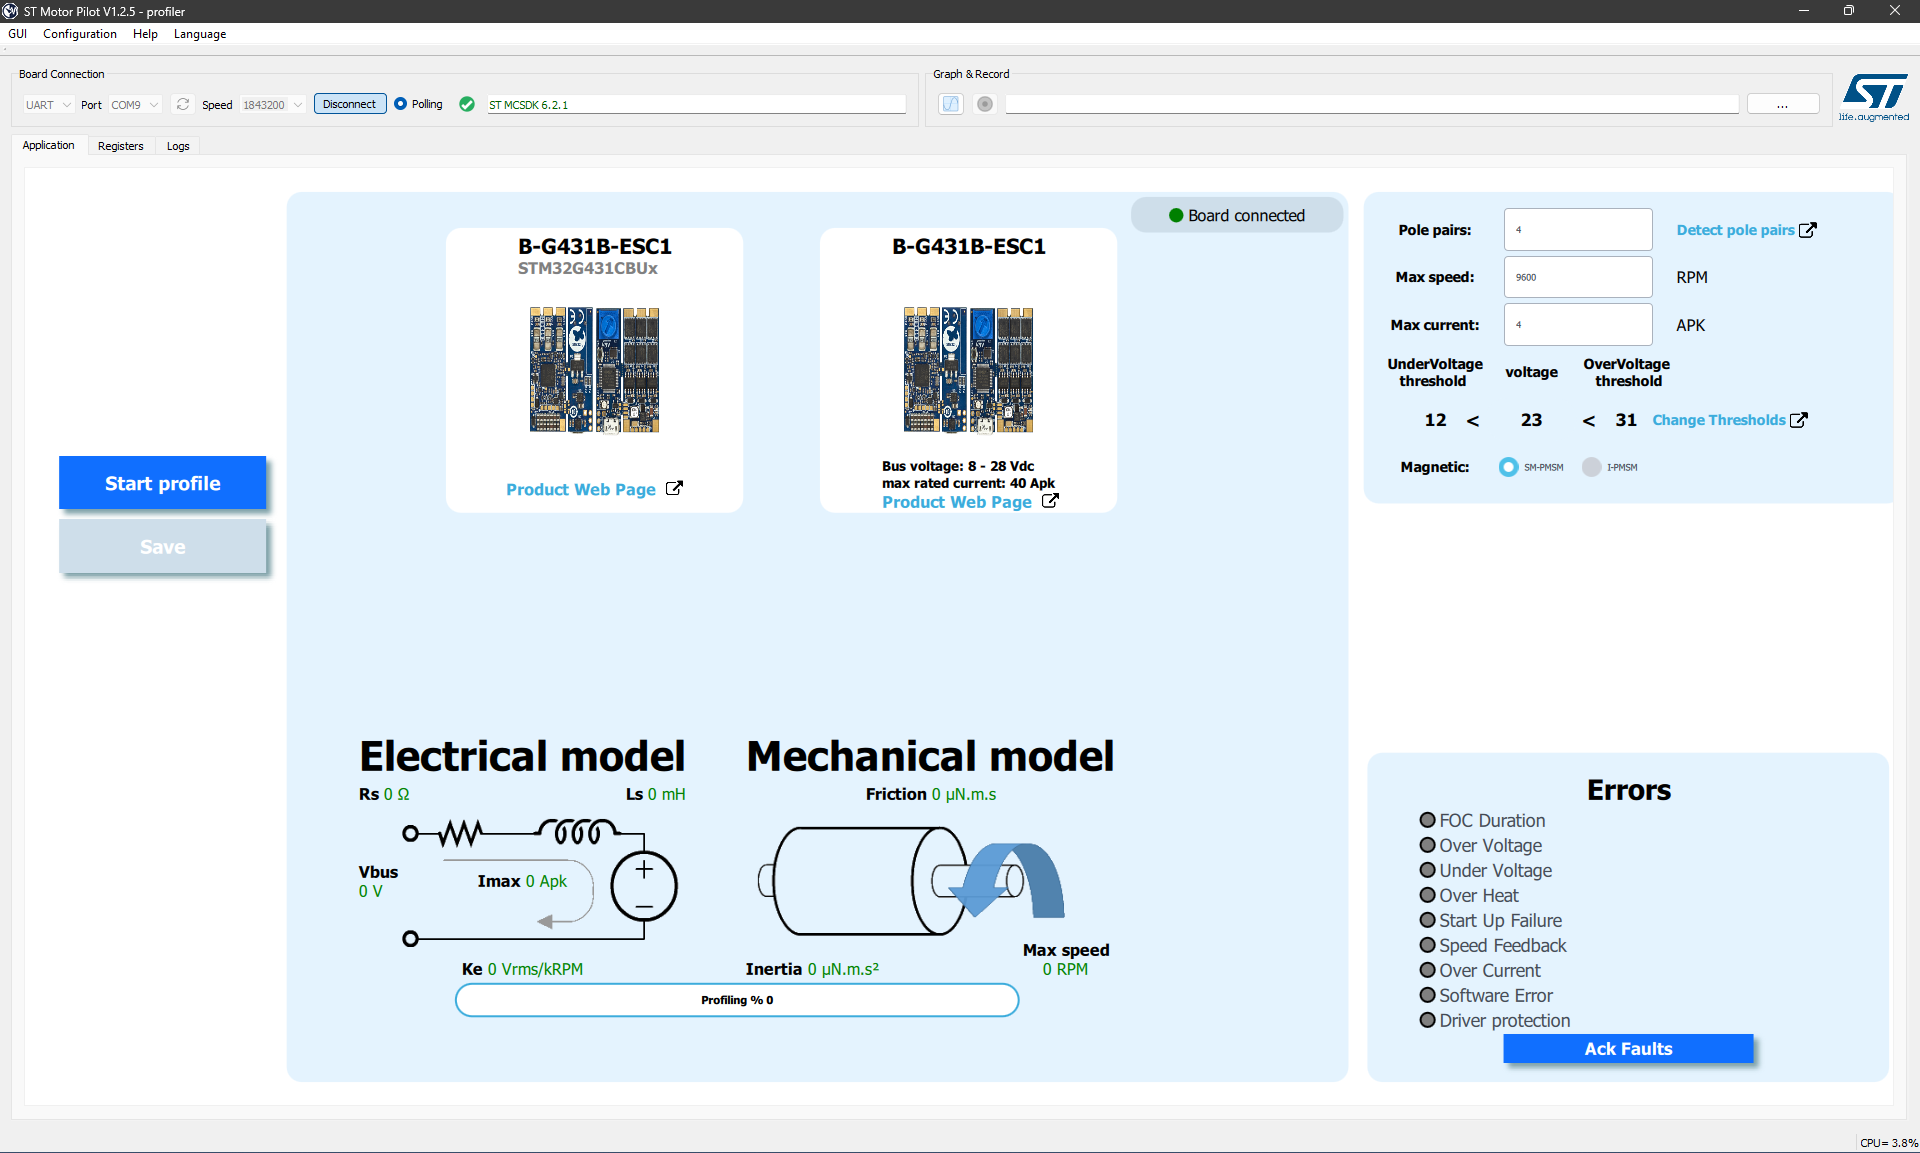
\includegraphics[width=\textwidth]{References/New Motor Profiler Parameters.png}}
                        \caption{Motor Profiler Filled Parameters}
                    \end{figure}
                \item Connect microcontroller to power supply set to 24V via soldered V+ and V- wires. Ensure that the motor is able to draw at least 4 amps.
                \item Select \emph{Start Profile}, this may take a while. After profile is done, ensure that you select \emph{Save} and name it something recognizable i.e. ElectroCraft RPX32. You will also need to add a description in the latest version.
            \end{itemize}
            It is possible (like in my case) that the profiled Inertia (or another parameter) is set to $0 uN*ms^2$. If this is the case, you will need to get the parameter from the 5.4.8 version of the profiler and input this parameter in \emph{MotorControl Workbench} under the \emph{Motor} section each time you start a new project.
		\FloatBarrier \subsection{Getting COM Port}
            \begin{itemize}
                \item Open Device Manager
                \item Expand \emph{Ports (COM \& LPT)}.
                \item Your COM Port is the one associated with \emph{STMicroelectronics STLink Virtual COM Port (COMX)}
            \end{itemize}
            \begin{figure}[H]
                \centerline{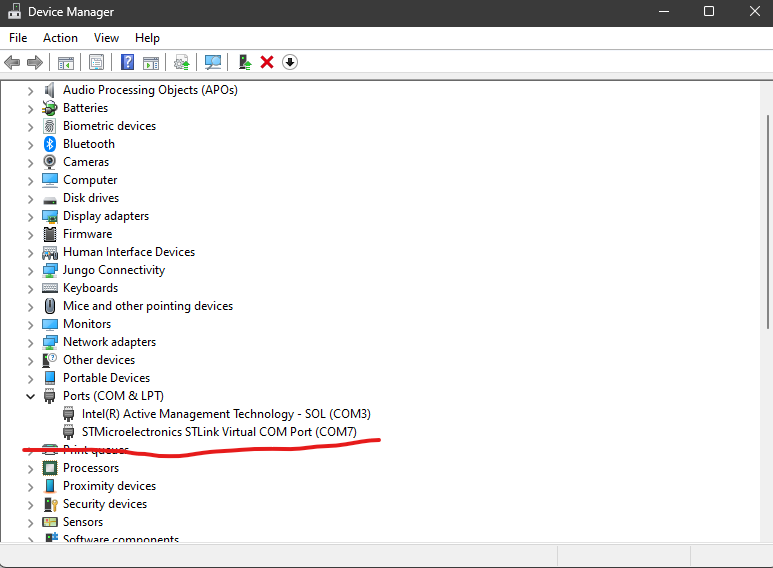
\includegraphics[width=\textwidth]{References/Device Manager COM Port.png}}
                \caption{Device Manager COM Port}
            \end{figure}
	\FloatBarrier \section{Getting Sensorless Motor Working}
		\FloatBarrier \subsection{GIT Code}
            To make working in this document easier, my versions of the below examples will be included in a git repository that you can download. You do not need to complete this step, but it may be useful for comparing your project to a completed one. \\
            \textbf{Branch} - Sensorless-MotorControl
		\FloatBarrier \subsection{MotorControl Workbench}
            \textbf{Commit} - bdafa29720fc13fdf07498f0b3aa8118d8e69f6c
            \begin{itemize}
                \item Open MotorControl Workbench (the latest version you have). 
                    \begin{figure}[H]
                        \centerline{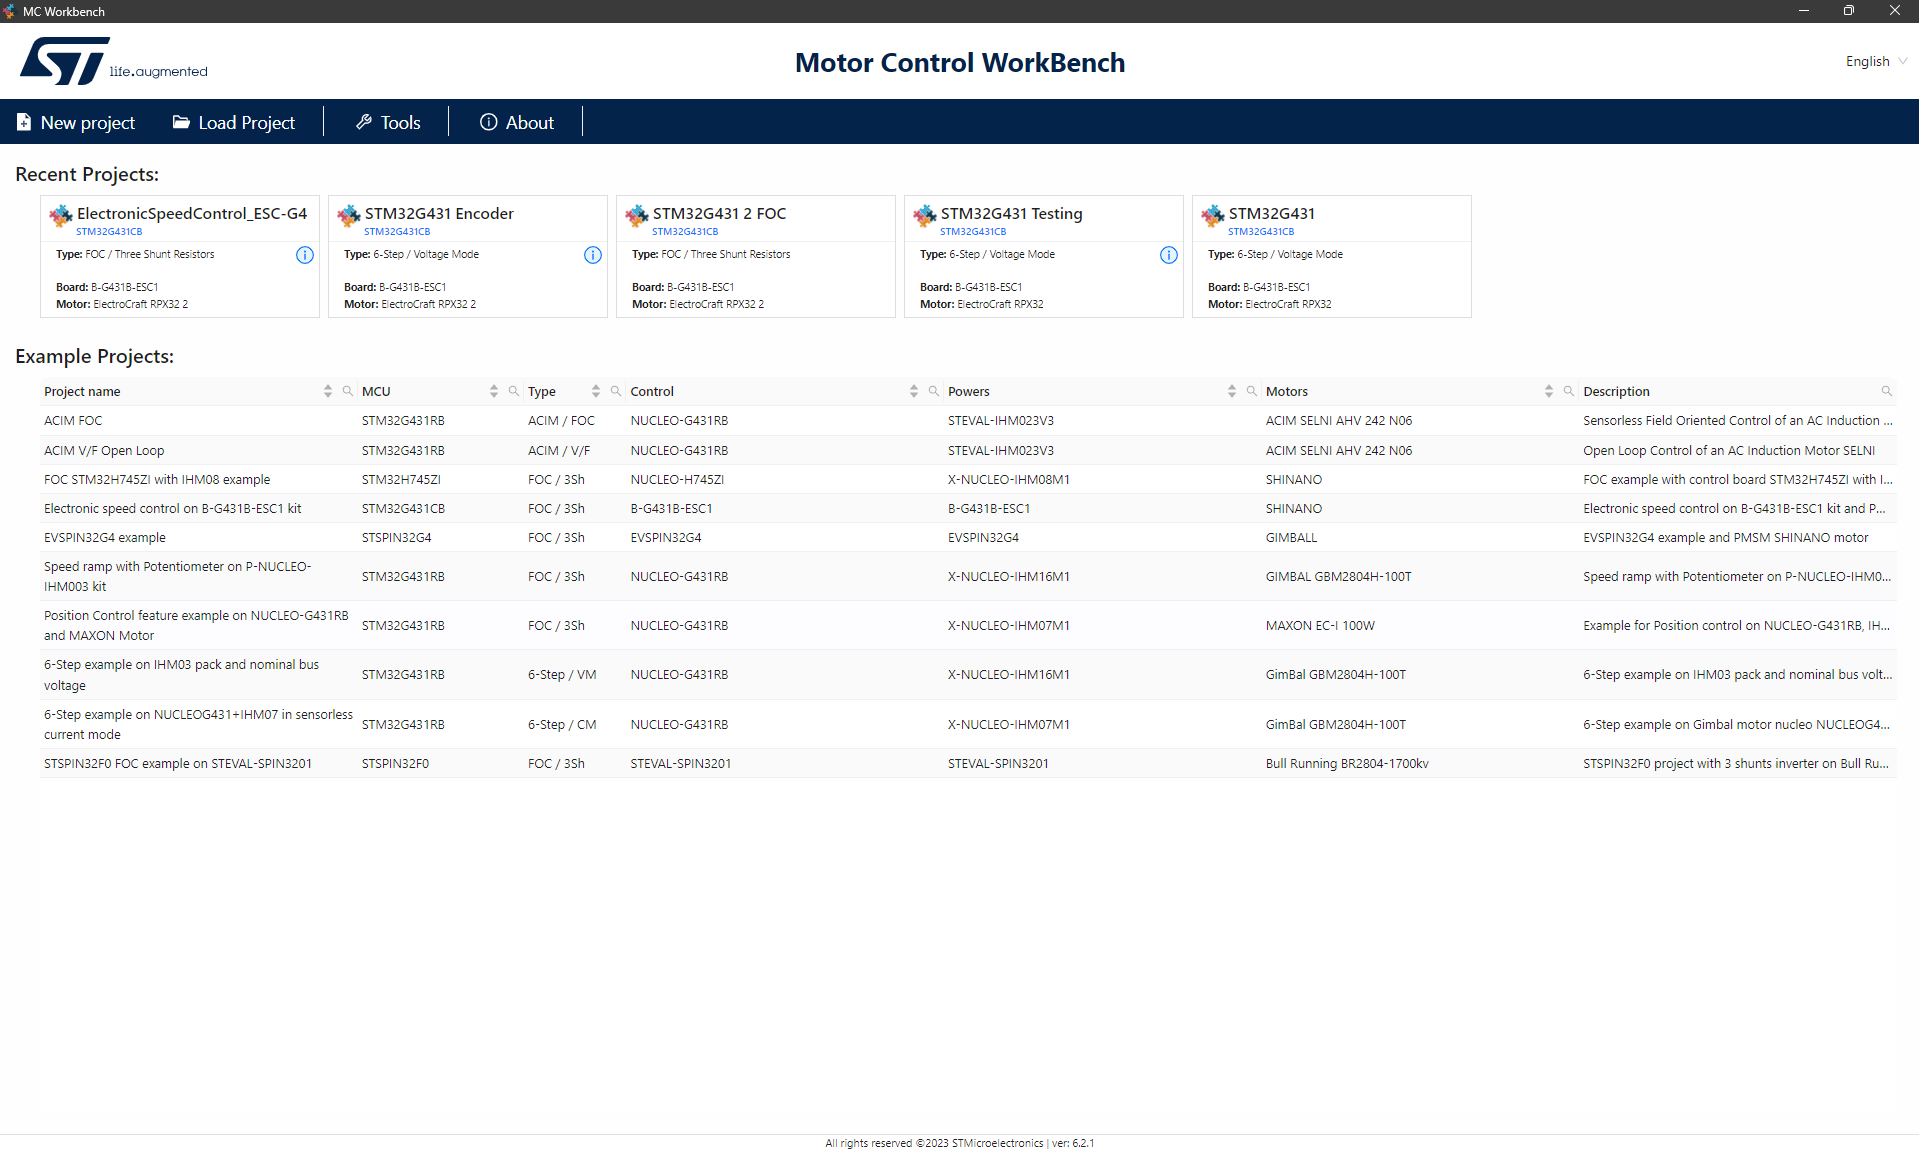
\includegraphics[width=\textwidth]{References/MC Workbench.png}}
                        \caption{MotorControl Workbench}
                    \end{figure}
                \item Select \emph{New project} in the top left.
                \item Give your project a name like "STM32G431 Sensorless Motor Control"
                \item \emph{Num. Motors} is 1 Motor, \emph{Driving Algorithm} is 6-Step, and \emph{Hardware Mode} is Inverter. Click Next at the bottom right.
                    \begin{figure}[H]
                        \centerline{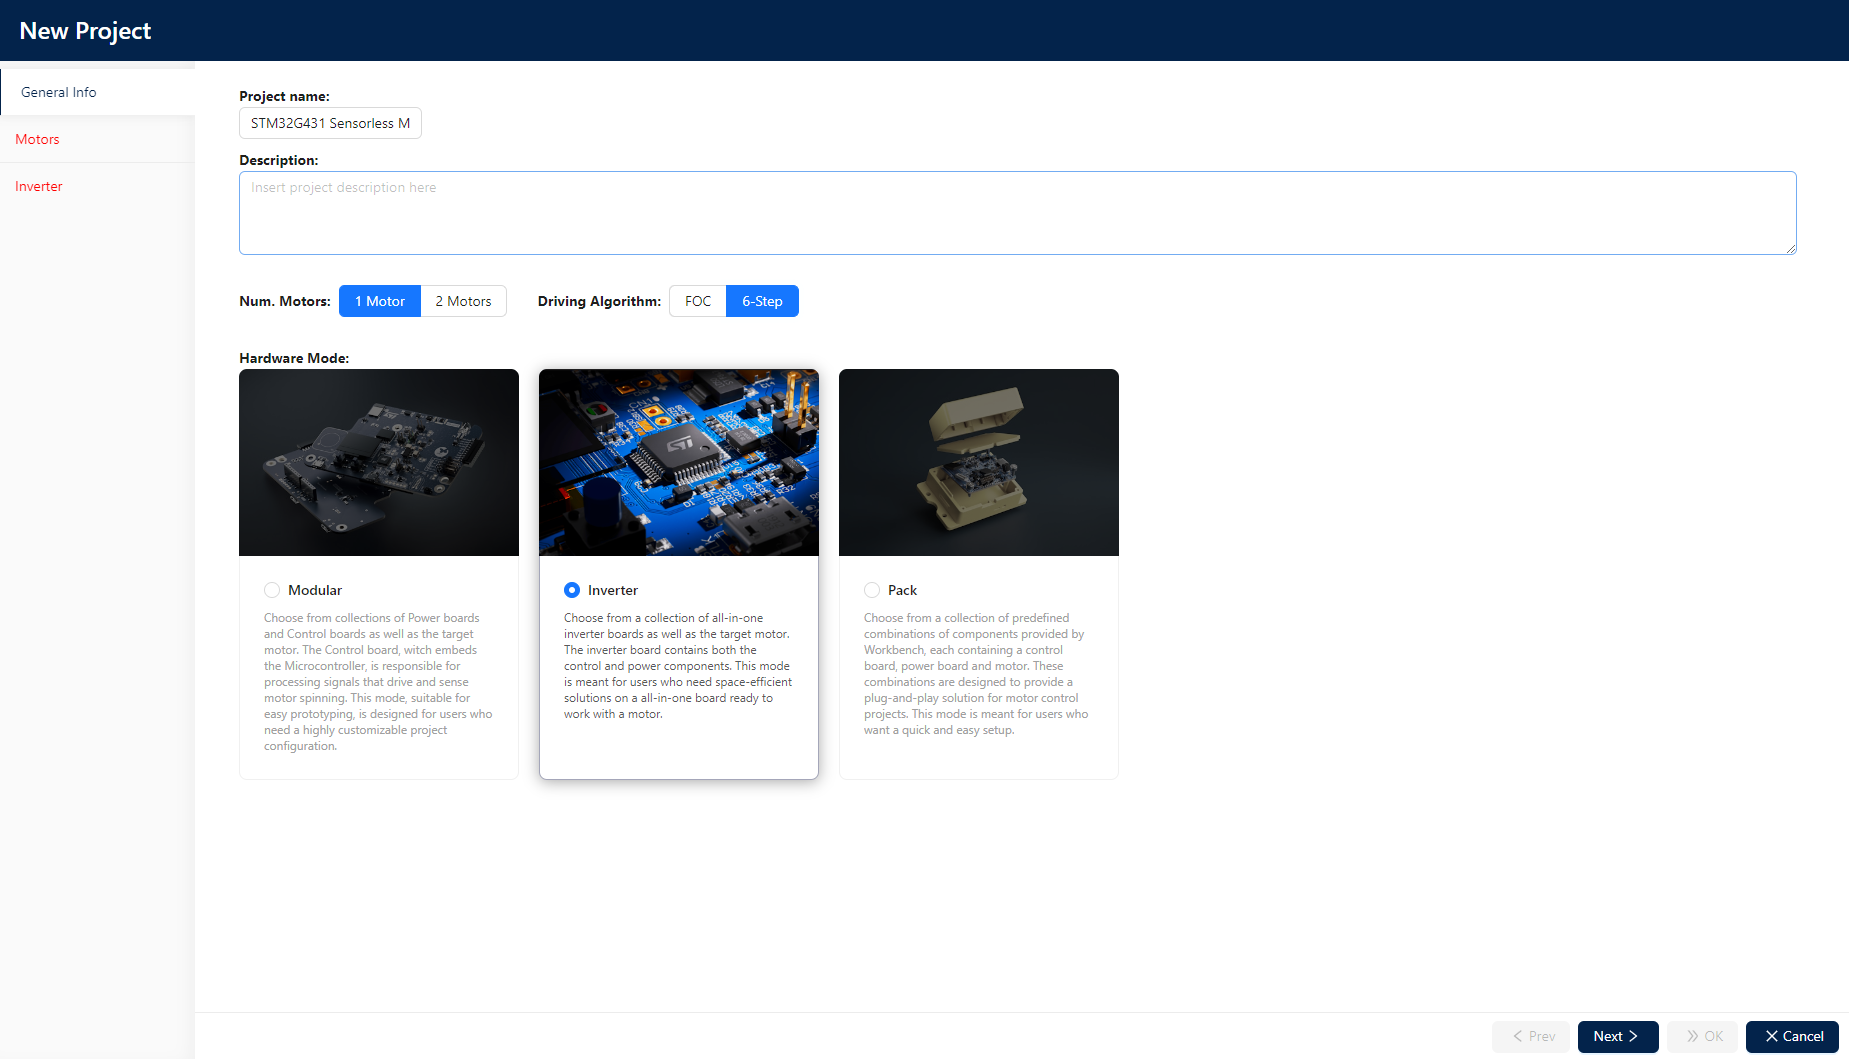
\includegraphics[width=\textwidth]{References/MCW Sensorless New Project.png}}
                        \caption{MotorControl Workbench New Project}
                    \end{figure}
                \item Select the Motor you profiled in the previous section. Click Next
                \item Select B-G431B-ESC1 as your board. Click OK.
                \item This will bring you to the MotorControl Workbench Project screen. Nothing needs to be done on this screen other than click \emph{Generate the project} at the top of the screen and save it.
                    \begin{figure}[H]
                        \centerline{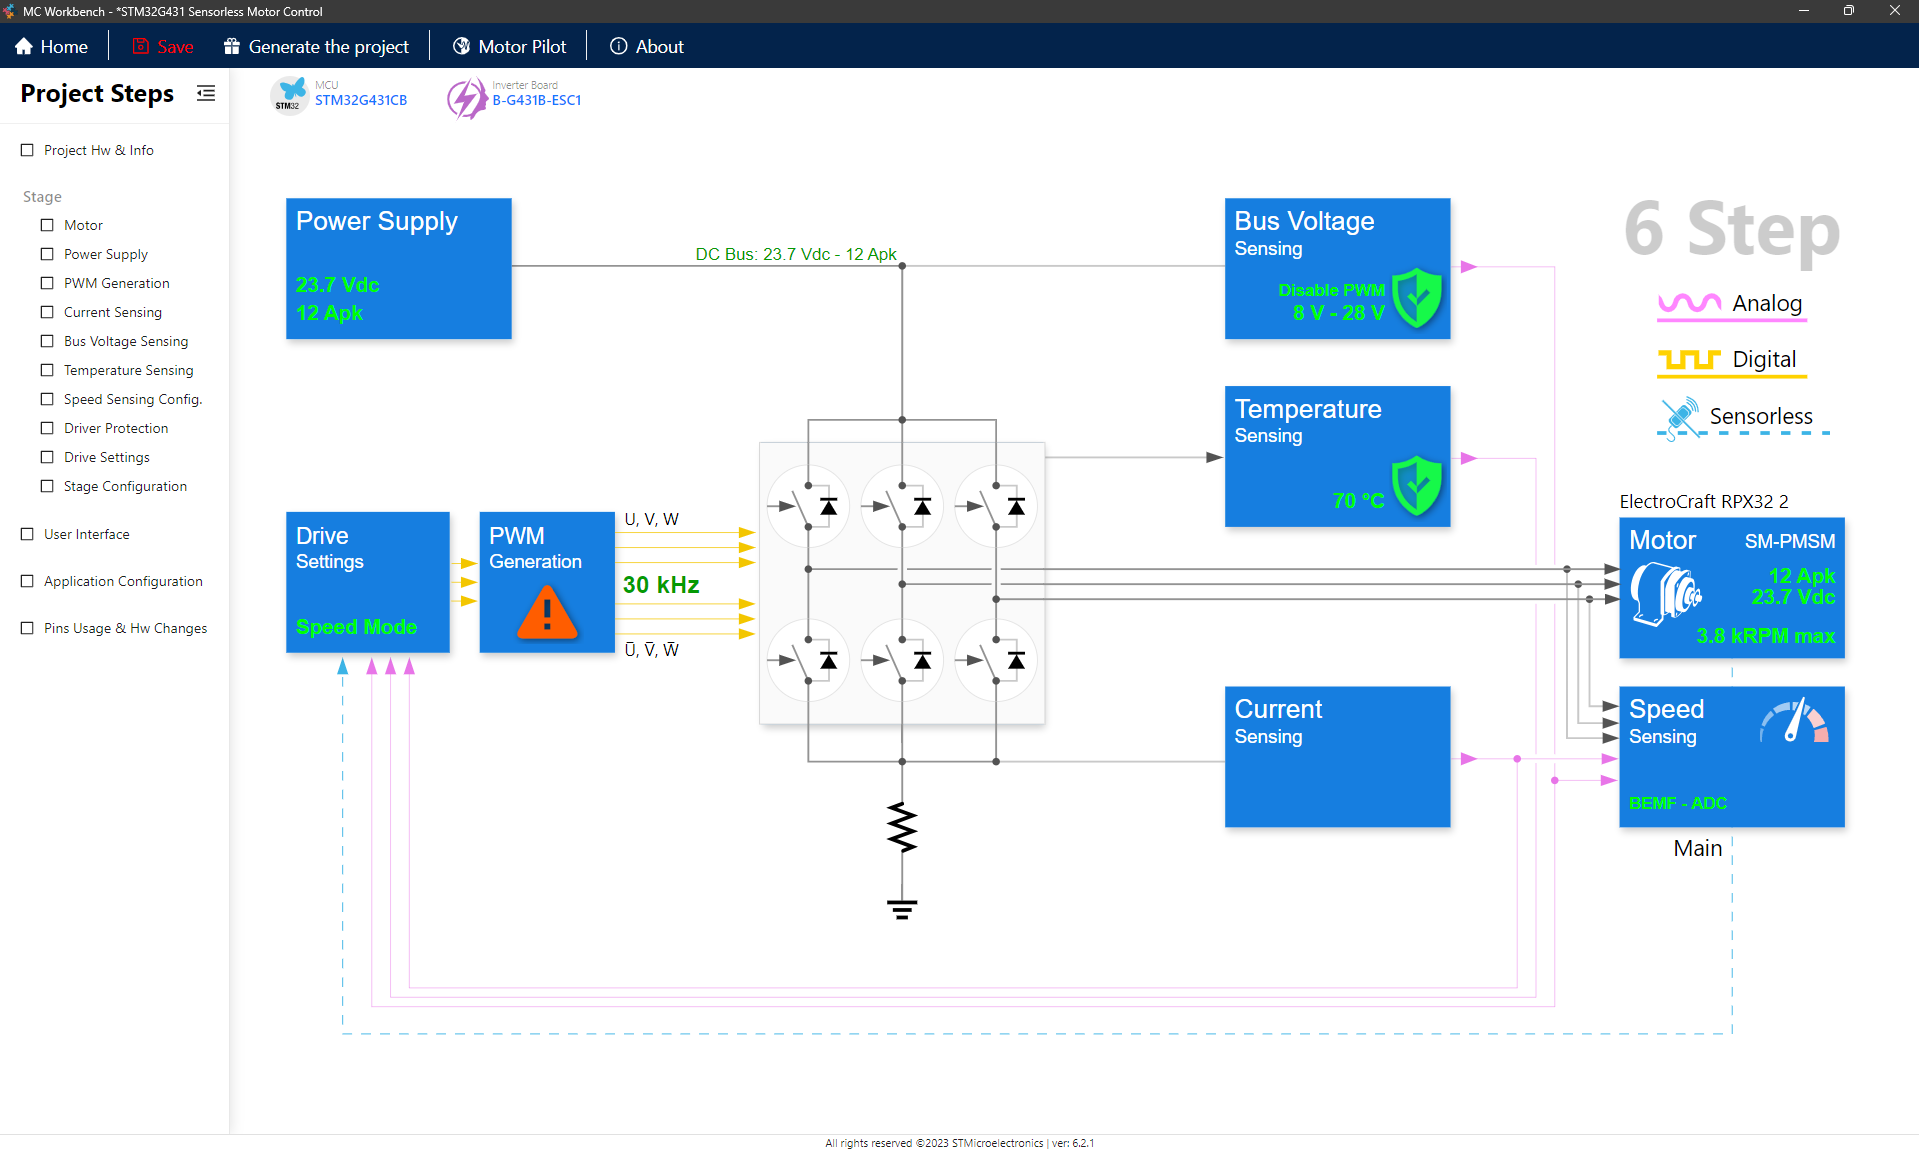
\includegraphics[width=\textwidth]{References/MCW Project Screen.png}}
                        \caption{MotorControl Workbench Project Screen}
                    \end{figure}
                \item Next the \emph{Project generation} screen will appear. Select the latest version of STM32CubeMX as your \emph{STM32CubeMX} version, select \emph{IAR EWARM V8} as your \emph{Target Toolchain}, and leave the recommended firmware under \emph{Firmware Package Version} and \emph{HAL - Hardware Abstraction Layer} as \emph{Drive Type}.
                    \begin{figure}[H]
                        \centerline{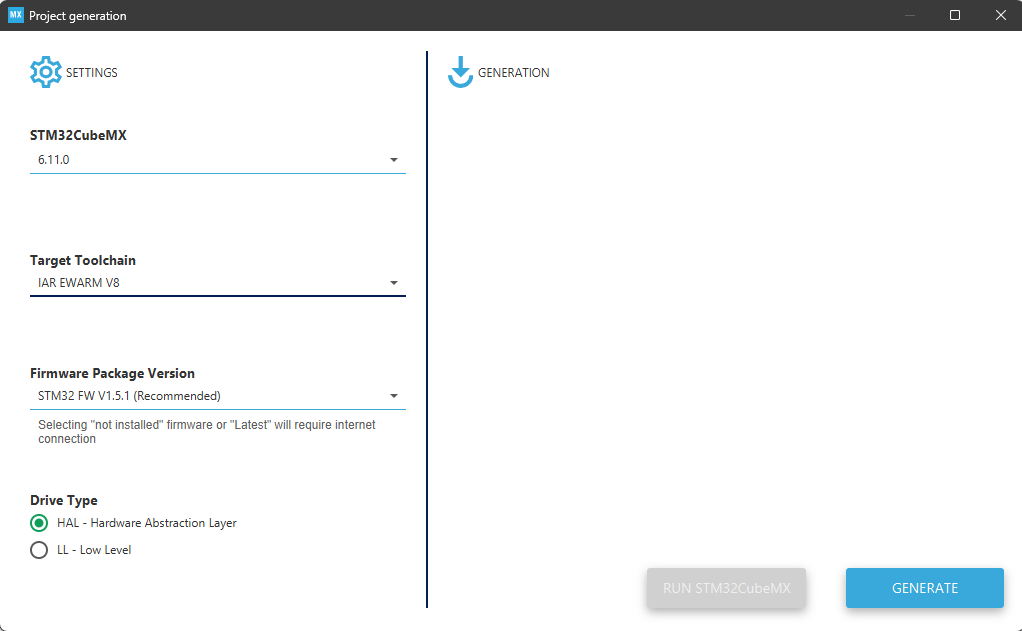
\includegraphics[width=\textwidth]{References/MCW Project Gen.png}}
                        \caption{MotorControl Workbench Project Generation Screen}
                    \end{figure}
                \item Select \emph{GENERATE}. It may ask you to install firmware, do so if prompted.
                \item Once completed, select \emph{RUN STM32CubeMX}.
            \end{itemize}
		\FloatBarrier \subsection{STM32CubeMX}
            The only thing required to do in STM32CubeMX is click \emph{GENERATE CODE} in the top right and then \emph{Open Project} when completed. You may be tempted to skip this step is subsequent runs as MotorControl Workbench will automatically regenerate some code, but if anything involving the ports needs to be updated, STM32CubeMX will need to be run.
            \begin{figure}[H]
                \centerline{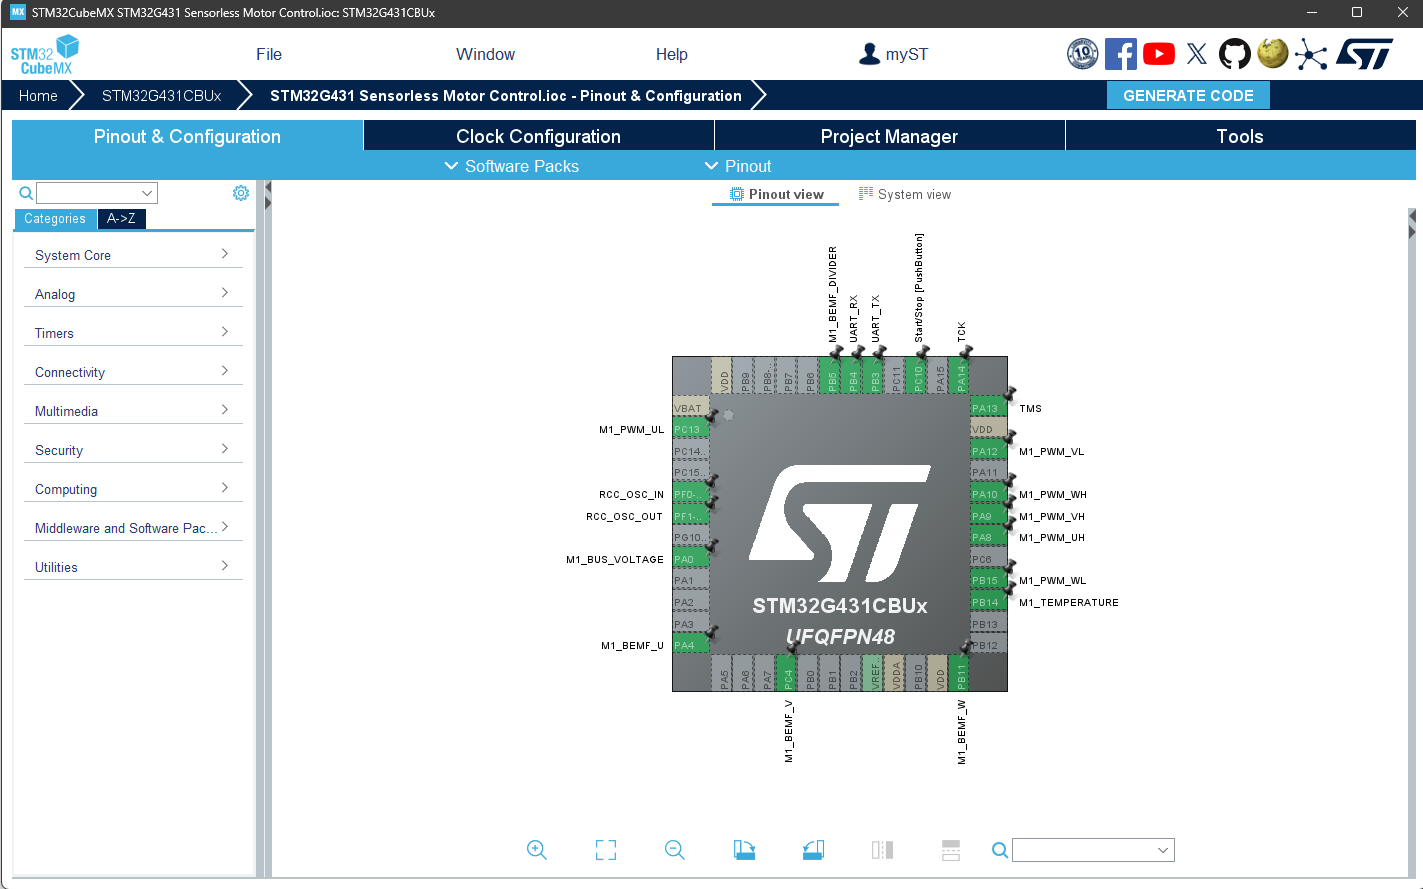
\includegraphics[width=\textwidth]{References/CubeMX.png}}
                \caption{STM32CubeMX Project Screen}
            \end{figure}
		\FloatBarrier \subsection{IAR EW for ARM}
            A screen will pop up asking if you would like to upgrade the project to the latest IAR version. Do so. You can compile and download the project to the board in IAR using the green button with a white triangle. You can turn on and off the motor using the button on the control board.
			\FloatBarrier \subsubsection{Motor Functions}
                There are three main functions used in the operation of the motor in this section.
                \begin{enumerate}
                    \item \texttt{MC\_StartMotor1(void)} - Starts the motor.
                    \item \texttt{MC\_StopMotor1(void)} - Stops the motor
                    \item \texttt{MC\_ProgramSpeedRampMotor1\_F(float\_t FinalSpeed, uint16\_t hDurationms)} - Select motor rotation speed. \texttt{FinalSpeed} is in RPM, the sign of this number is the rotation direction. \texttt{hDurationms} is number of milliseconds it will take the motor to reach this speed. 0 is follow mode which I have found to not be very accurate, the minimum I would set this is 20 ms.
                \end{enumerate}
			\FloatBarrier \subsubsection{While Loop Motor Operation}
                \textbf{Commit} - 5b851c28c37d08e9c23311cba398b17b16715040 \\
                When code is generated by the MotorControl Workbench or STM32CubeMX, there will be \texttt{/* USER CODE */} around sections that will survive from one generation to the next. Additionally we can use the function \texttt{HAL\_Delay(delay\_ms)} to insert a delay between operations. Therefore the code 
                \begin{verbatim}
while (1)
{
    /* USER CODE END WHILE */

    /* USER CODE BEGIN 3 */
    MC_StartMotor1();
    HAL_Delay(2000);
    MC_StopMotor1();
    HAL_Delay(400);
}
                \end{verbatim}
                will start the motor, delay by 2000 ms (2 seconds), stop the motor, delay by 400 ms, then loop back to the top. \\ 
                You should always set a speed before stating the motor for the first time. In the section labeled \texttt{/* USER CODE BEGIN 2 */}, insert
                \begin{verbatim}
/* USER CODE BEGIN 2 */
MC_ProgramSpeedRampMotor1_F(1500, 1000);

/* USER CODE END 2 */
                \end{verbatim}
                 This will set the motor to 1500 RPM after a 1000 ms (1 second) ramp up period. You can now compile, download, and run this code on your board. You will need to hit the white circle with blue arrow in it at the top of IAR to run the code. \\
                \textbf{Commit} - 6df35948c6d4056a369c20ab65d1e11f044f3218 \\
                A more interesting way to run the motor is to reverse its direction after ever start/stop. To do this, we can insert the\texttt{ MC\_ProgramSpeedRampMotor1} function after each stop, with a negative rotation every other start/stop.
                \begin{verbatim}
while (1)
{
    /* USER CODE END WHILE */

    /* USER CODE BEGIN 3 */
    MC_StartMotor1();
    HAL_Delay(2000);
    MC_StopMotor1();
    HAL_Delay(400);
    MC_ProgramSpeedRampMotor1_F(-1500, 1000);
    MC_StartMotor1();
    HAL_Delay(2000);
    MC_StopMotor1();
    HAL_Delay(400);
    MC_ProgramSpeedRampMotor1_F(1500, 1000);
}
                \end{verbatim}
                This will start the motor going the forward direction (because of the code in \texttt{/* USER CODE END 2 */}) then after it stops, start it going the other direction. It will then repeat. Mess around with the RPM and ramp up time to get a sense of how to use the motor. \emph{NOTE} I have empirically discovered that you need a 400 ms delay between stopping and starting the motor to get it to change direction. This is because the motor need to be in IDLE before it will change direction.
			\FloatBarrier \subsubsection{Button Motor Operation}
                \textbf{Commit} - 3d511c5de4201c02841dd940726a3afe4c0a3c74 \\
                By default, the MotorControl Workbench projects will default to starting and stopping motor with button press. You can try this out with the main loop, but your control will be overwritten quickly by the while loop. To change this, we can remove the code in the while loop and move parts of it further up the main function to where the previous speed initialization was. The code below will run the motor for 2 seconds and then stop it. Afterward, you are free to control the motor with the button on the board.
                \begin{verbatim}
/* USER CODE BEGIN 2 */
MC_ProgramSpeedRampMotor1_F(1500, 1000);
MC_StartMotor1();
HAL_Delay(2000);
MC_StopMotor1();

/* USER CODE END 2 */
                \end{verbatim}
                Build, download, run, and test this. \\ 
                You will notice that the motor does not reverse direction. To do this, we need to go into the \texttt{UI\_HandleStartStopButton\_cb} function in \texttt{mc\_tasks.c}. We need a variable to keep track to the previous direction and a control statement to decide which direction the motor should be running. Since we start motor in forward direction, we should reverse direction on first pass.
                \begin{verbatim}
__weak void UI_HandleStartStopButton_cb (void)
{
/* USER CODE BEGIN START_STOP_BTN */
    static bool direction = 0;
  if (IDLE == MC_GetSTMStateMotor1())
  {
    /* Ramp parameters should be tuned for the actual motor */
    if (direction == 0)
    {
        MC_ProgramSpeedRampMotor1_F(-1500, 1000);
        direction = 1;
    }
    else
    {
        MC_ProgramSpeedRampMotor1_F(1500, 1000);
        direction = 0;
    }

    (void)MC_StartMotor1();
  }
  else
  {
    (void)MC_StopMotor1();
  }
/* USER CODE END START_STOP_BTN */
}
                \end{verbatim}
                Build, run, and test this code. This allows you to be in control of what direction the motor is running and how long it is running for, great for testing the motor in a real world scenario.
	\FloatBarrier \section{Getting Hall-Effect Motor Working}
        Much of the below section is a copy paste of the \emph{Getting Sensorless Motor Working} section. The only different aspects are the wiring required, the MotorControl Workbench configuration, and the git branch. But the user added code itself is the same. 
		\FloatBarrier \subsection{Wiring Up Hall-Effect Sensor Lines}
            \begin{figure}[H]
                \centerline{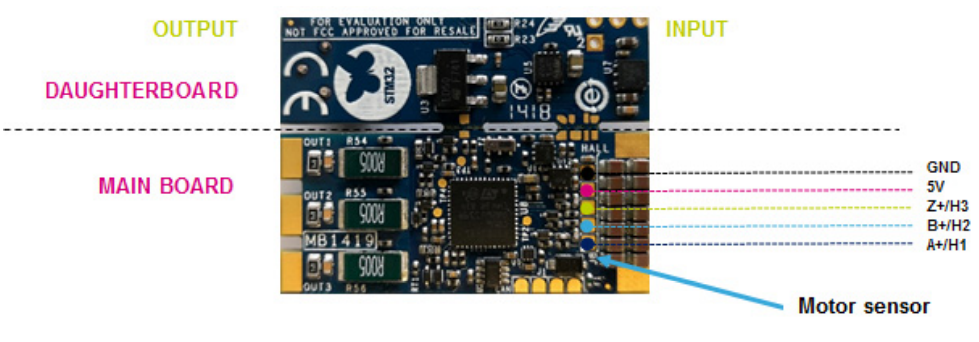
\includegraphics[width=\textwidth]{References/Sensor Wiring.png}}
                \caption{Board Sensor Wiring}
            \end{figure}
            \begin{figure}[H]
                \centerline{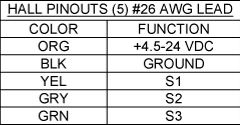
\includegraphics[width=\textwidth]{References/Hall-Effect Wiring.png}}
                \caption{Hall-Effect Wiring}
            \end{figure}
            \begin{figure}[H]
                \centerline{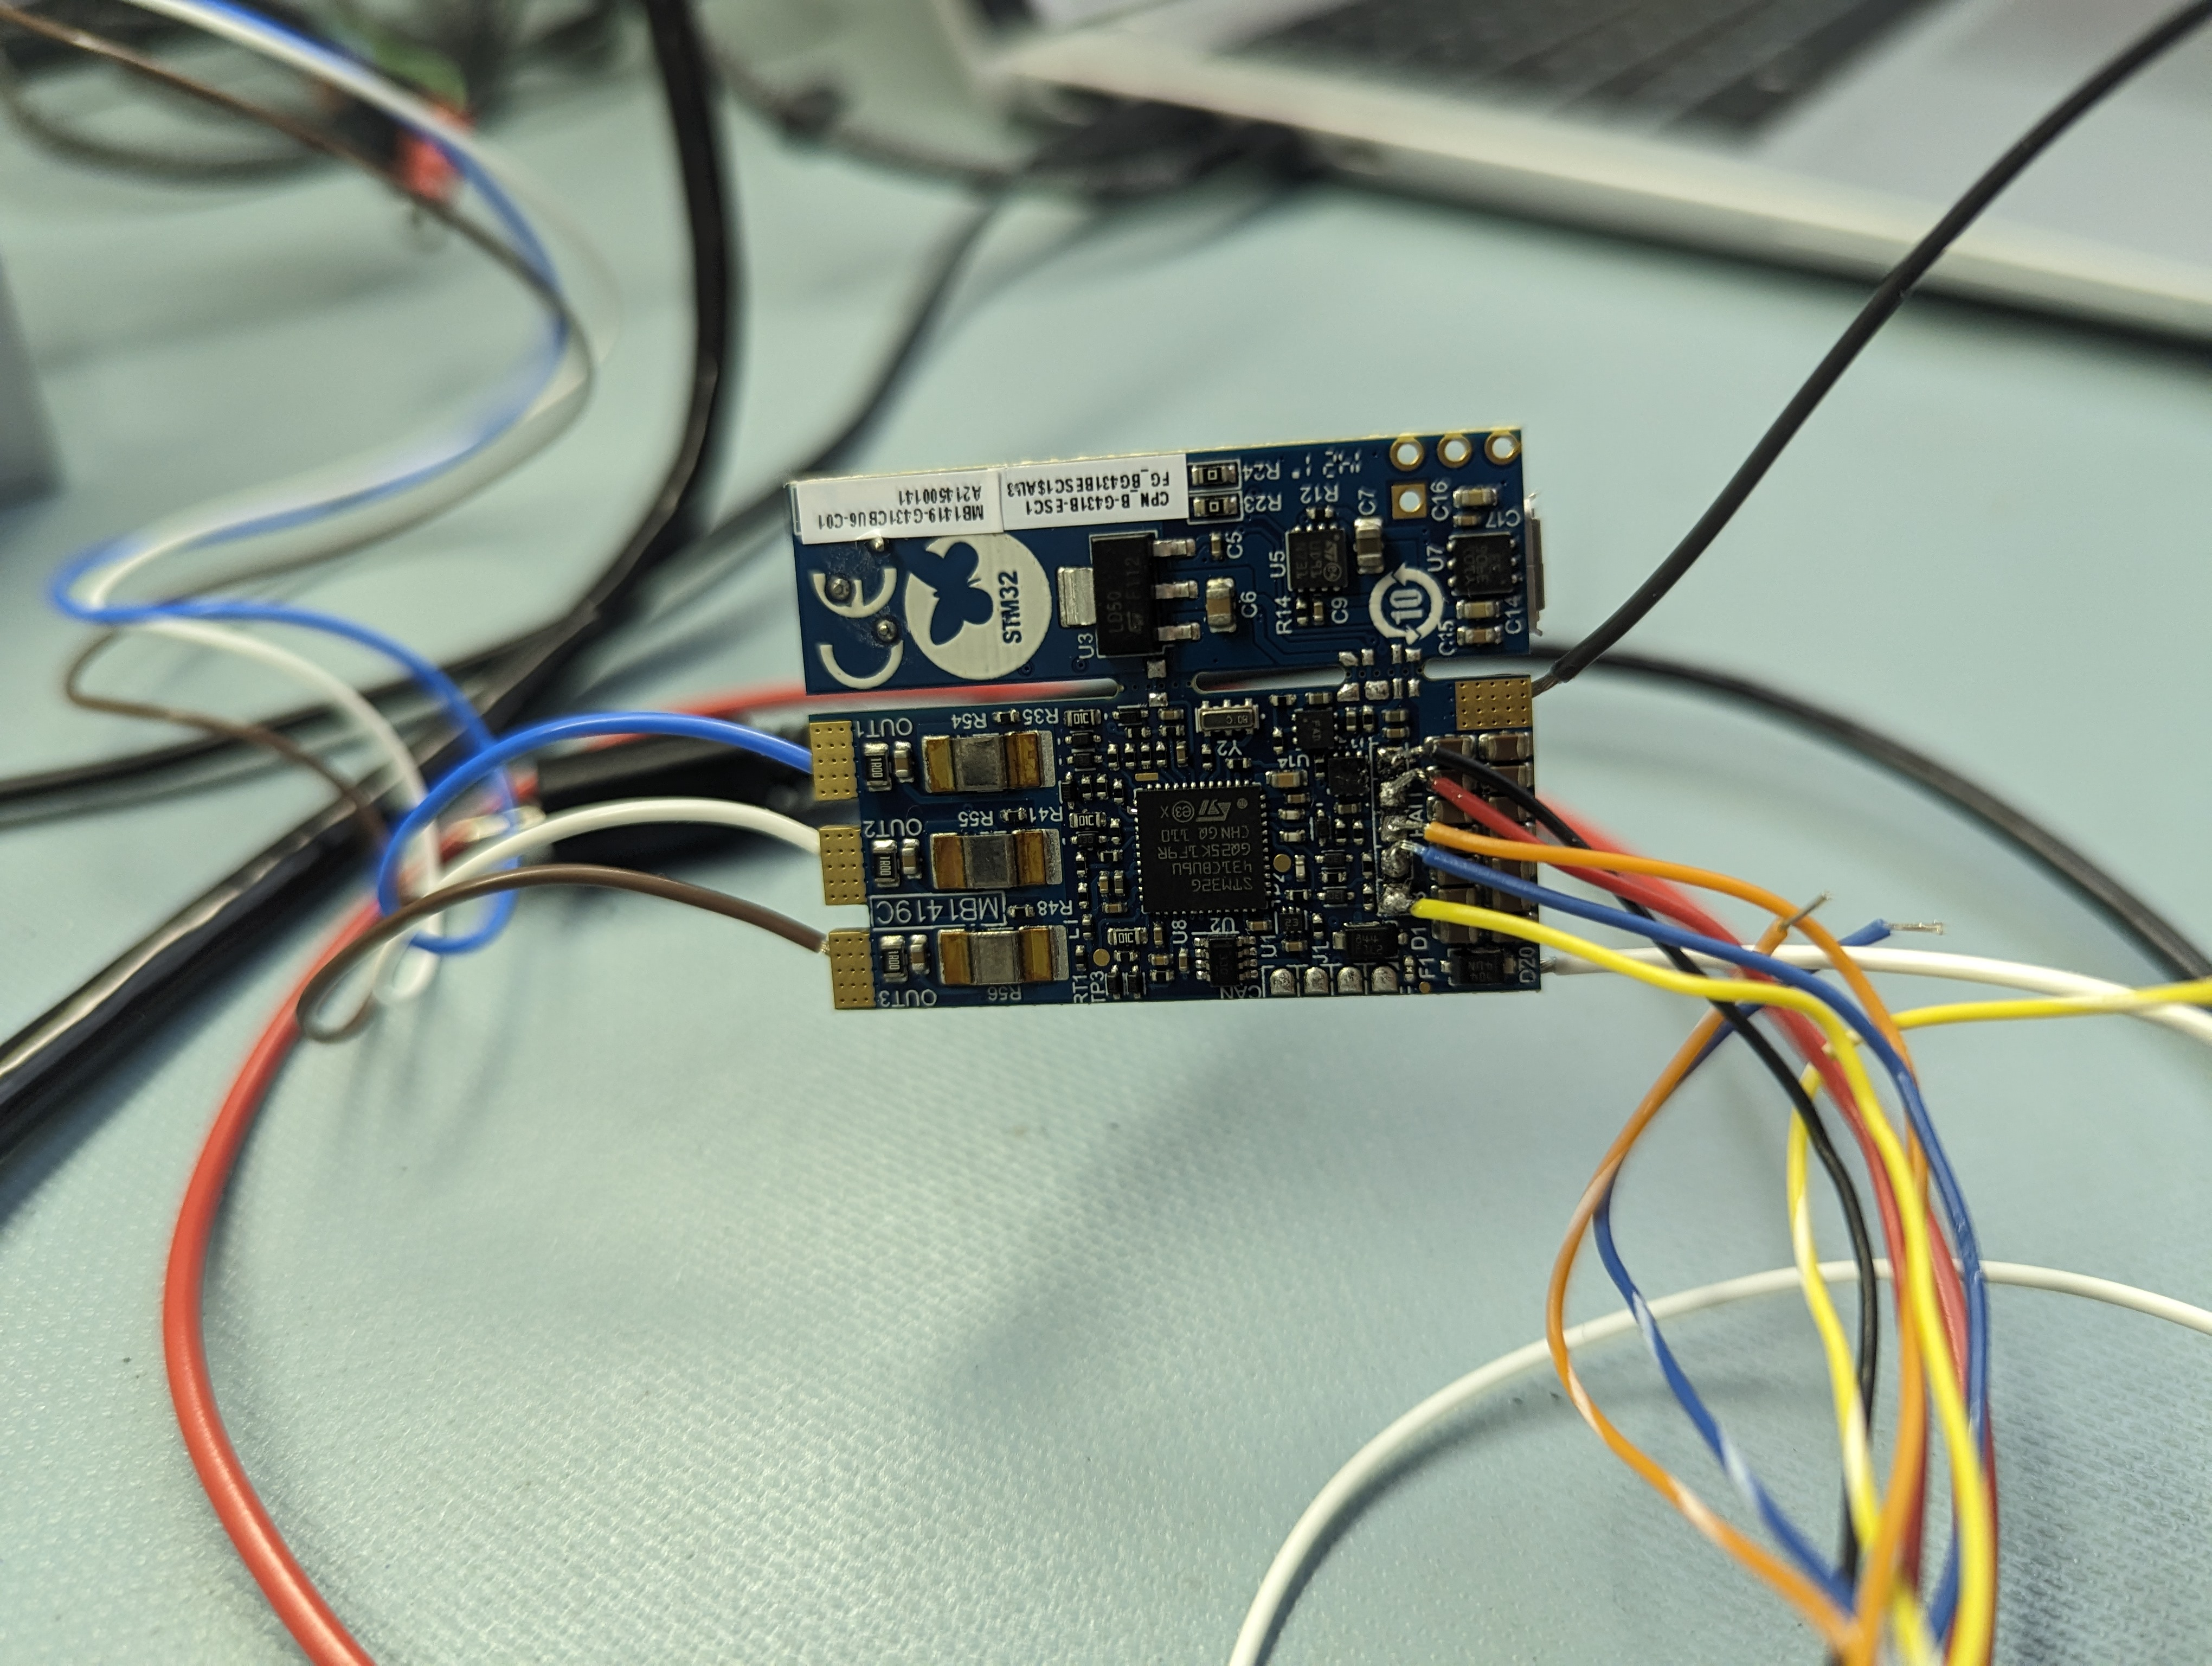
\includegraphics[width=\textwidth]{References/Hall-Effect Wiring Board Picture.jpg}}
                \caption{Hall-Effect Wiring Board Picture}
            \end{figure}
		\FloatBarrier \subsection{GIT Code}
            To make working in this document easier, my versions of the below examples will be included in a git repository that you can download. You do not need to complete this step, but it may be useful for comparing your project to a completed one. \\
            \textbf{Branch} - Hall-Effect-MotorControl
		\FloatBarrier \subsection{MotorControl Workbench}
        \textbf{Commit} - b92852f9cba090494cca2b5e58b5ad11a4efcd1f \\
            \begin{itemize}
                \item Open MotorControl Workbench (the latest version you have). 
                    \begin{figure}[H]
                        \centerline{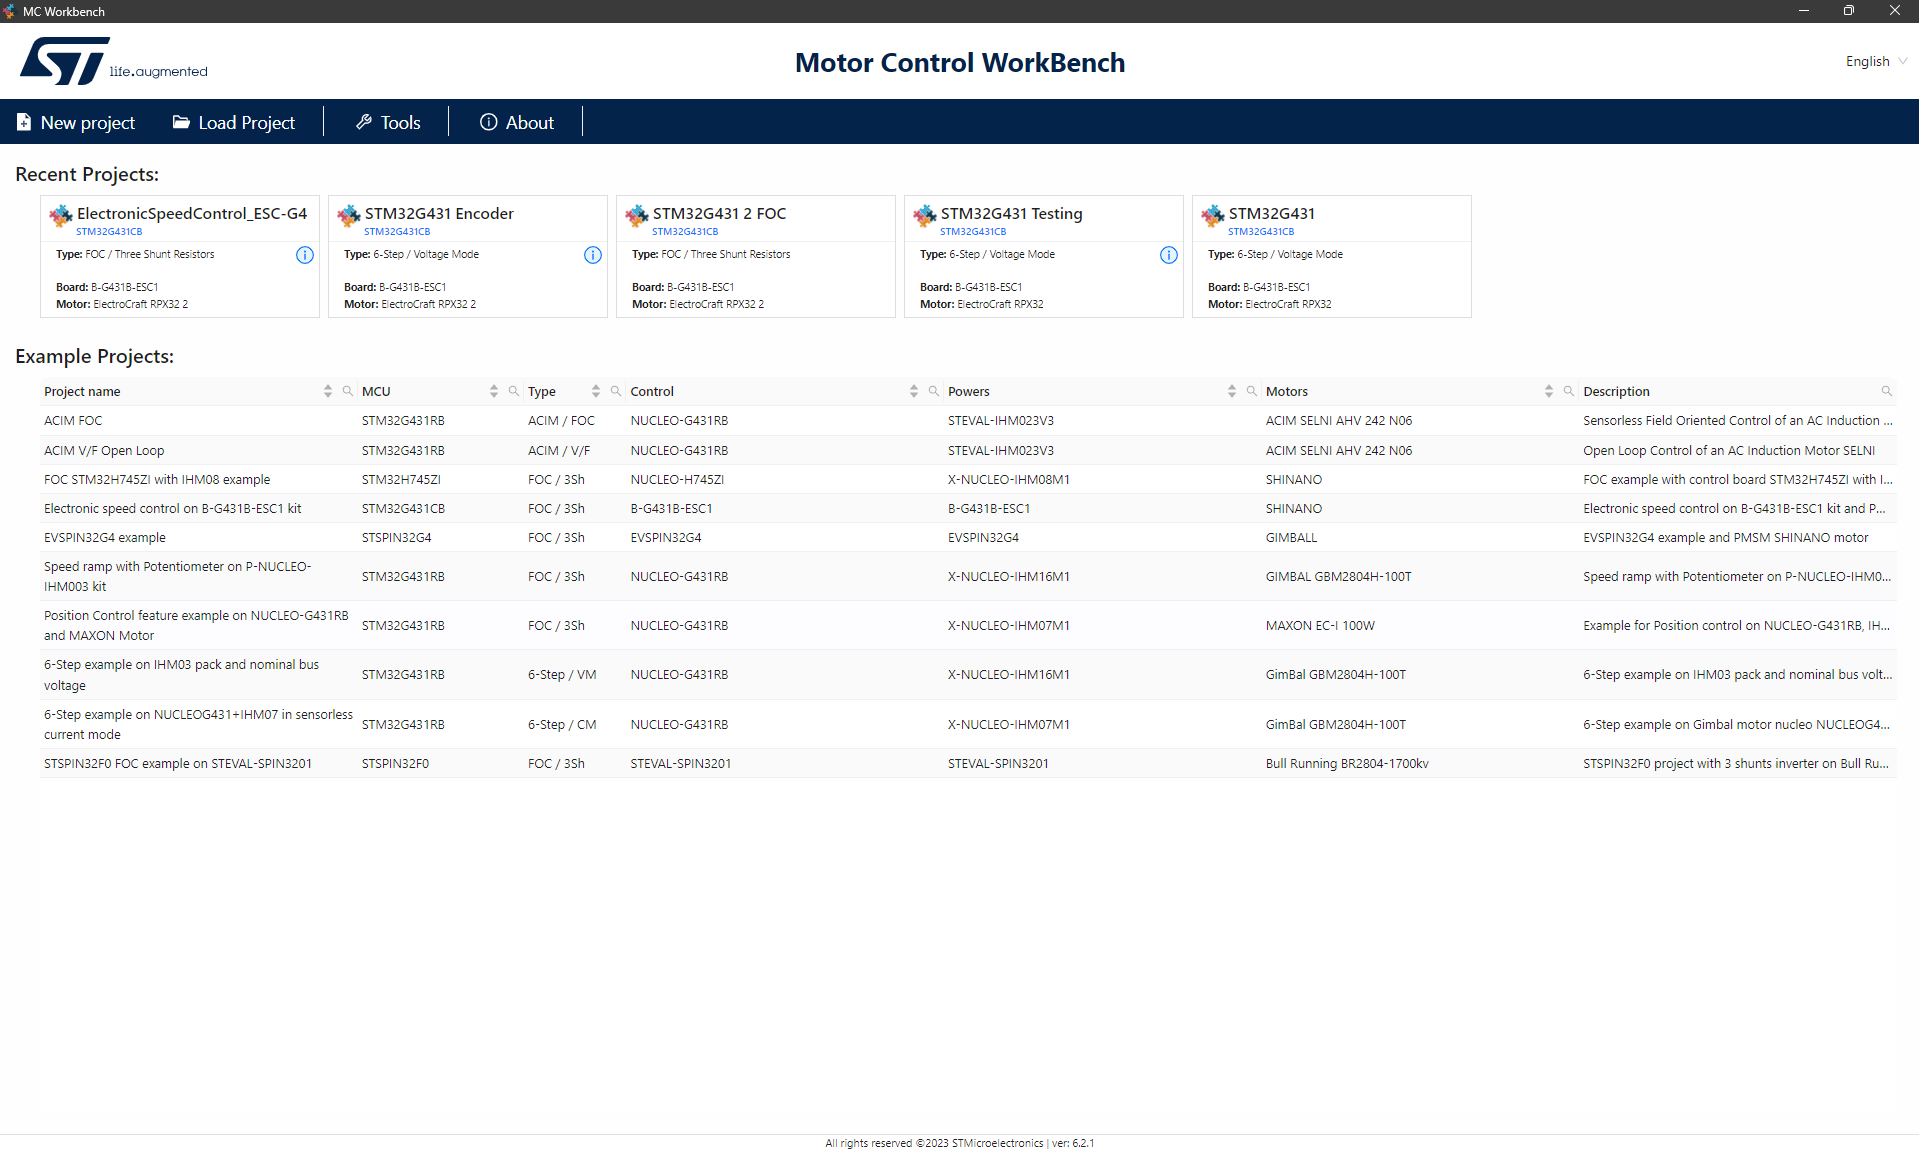
\includegraphics[width=\textwidth]{References/MC Workbench.png}}
                        \caption{MotorControl Workbench}
                    \end{figure}
                \item Select \emph{New project} in the top left.
                \item Give your project a name like "STM32G431 Hall-Effect Motor Control"
                \item \emph{Num. Motors} is 1 Motor, \emph{Driving Algorithm} is 6-Step, and \emph{Hardware Mode} is Inverter. Click Next at the bottom right.
                    \begin{figure}[H]
                        \centerline{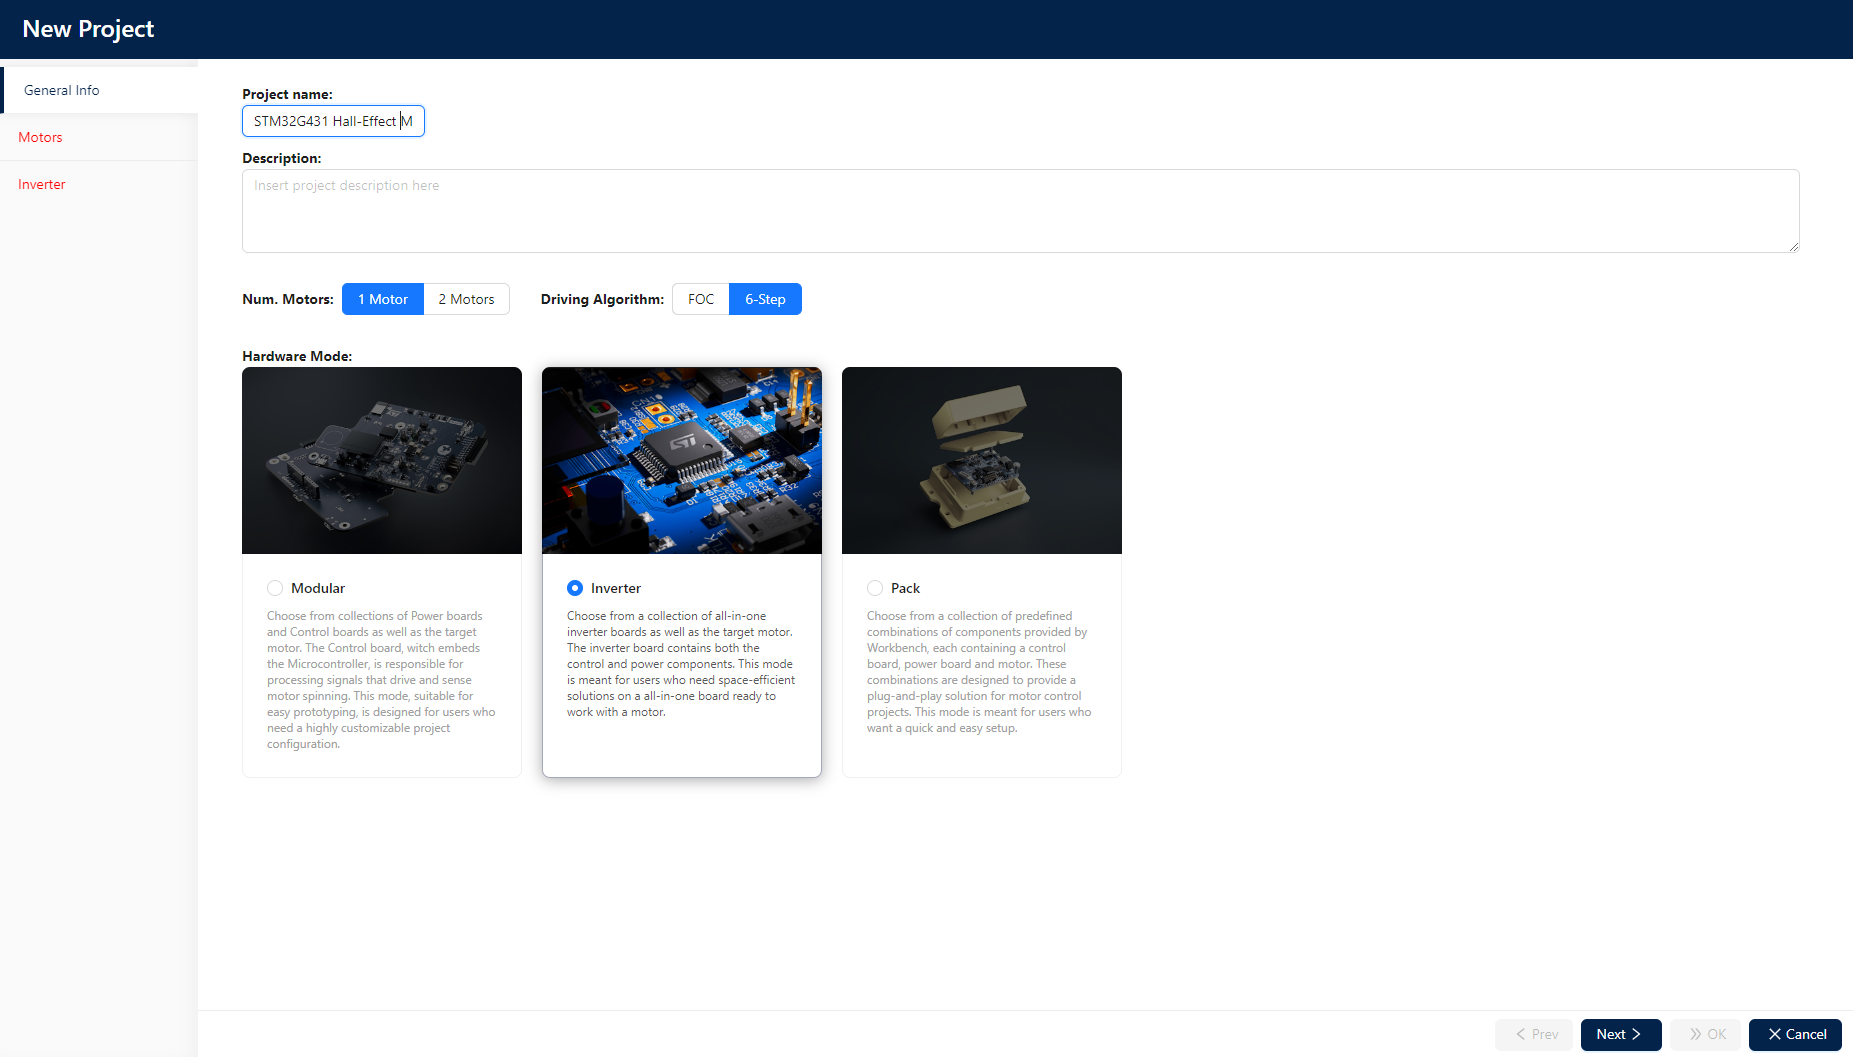
\includegraphics[width=\textwidth]{References/MCW Hall-Effect New Project.png}}
                        \caption{MotorControl Workbench New Project}
                    \end{figure}
                \item Select the Motor you profiled in the previous section. Click Next
                \item Select B-G431B-ESC1 as your board. Click OK.
                \item This will bring you to the MotorControl Workbench Project screen. 
                    \begin{figure}[H]
                        \centerline{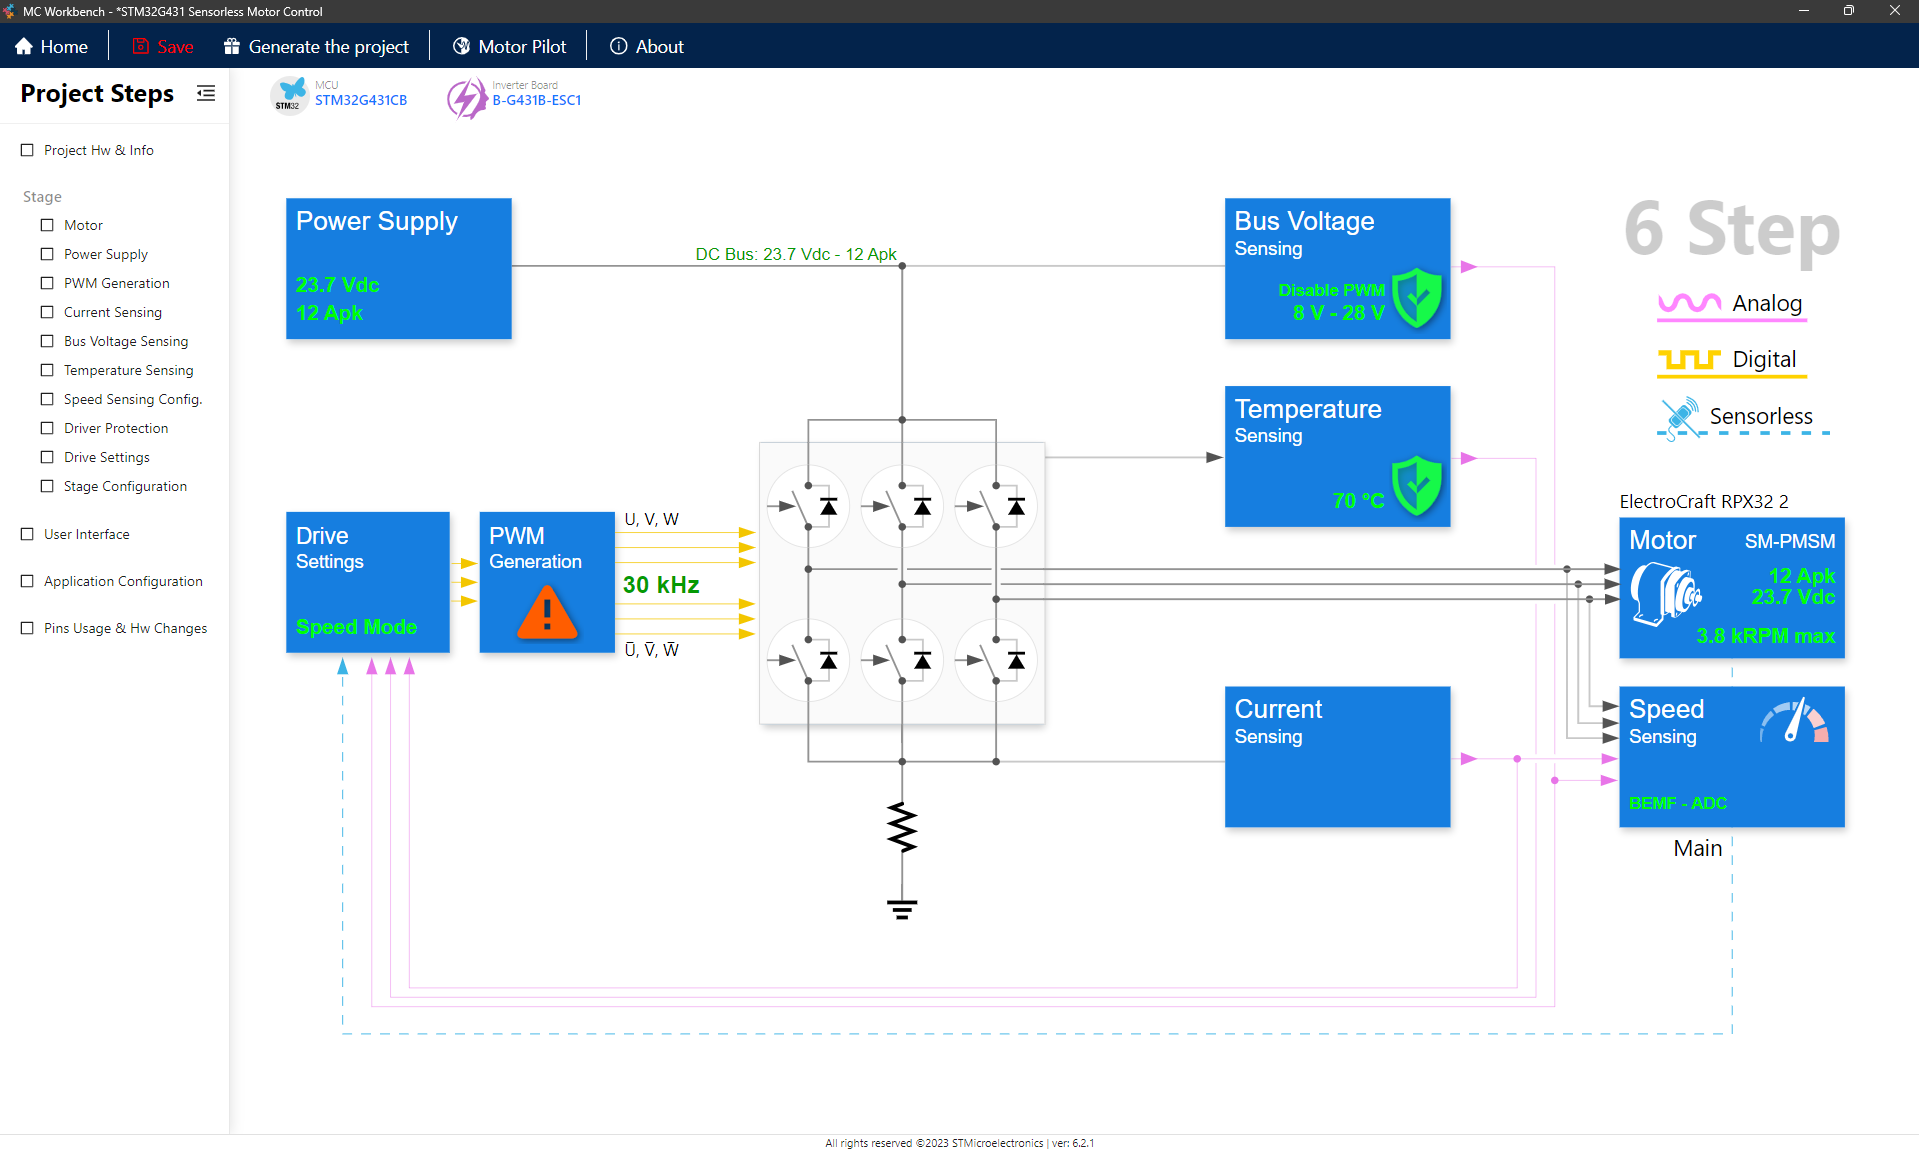
\includegraphics[width=\textwidth]{References/MCW Project Screen.png}}
                        \caption{MotorControl Workbench Project Screen}
                    \end{figure}
                \item From here, either click on \emph{Motor} on the left hand side or click the motor on the right hand side. Scroll down on this page to where is says \emph{Hall Effect} and turn this on and make sure \emph{Sensor displacement} is set to 120.
                    \begin{figure}[H]
                        \centerline{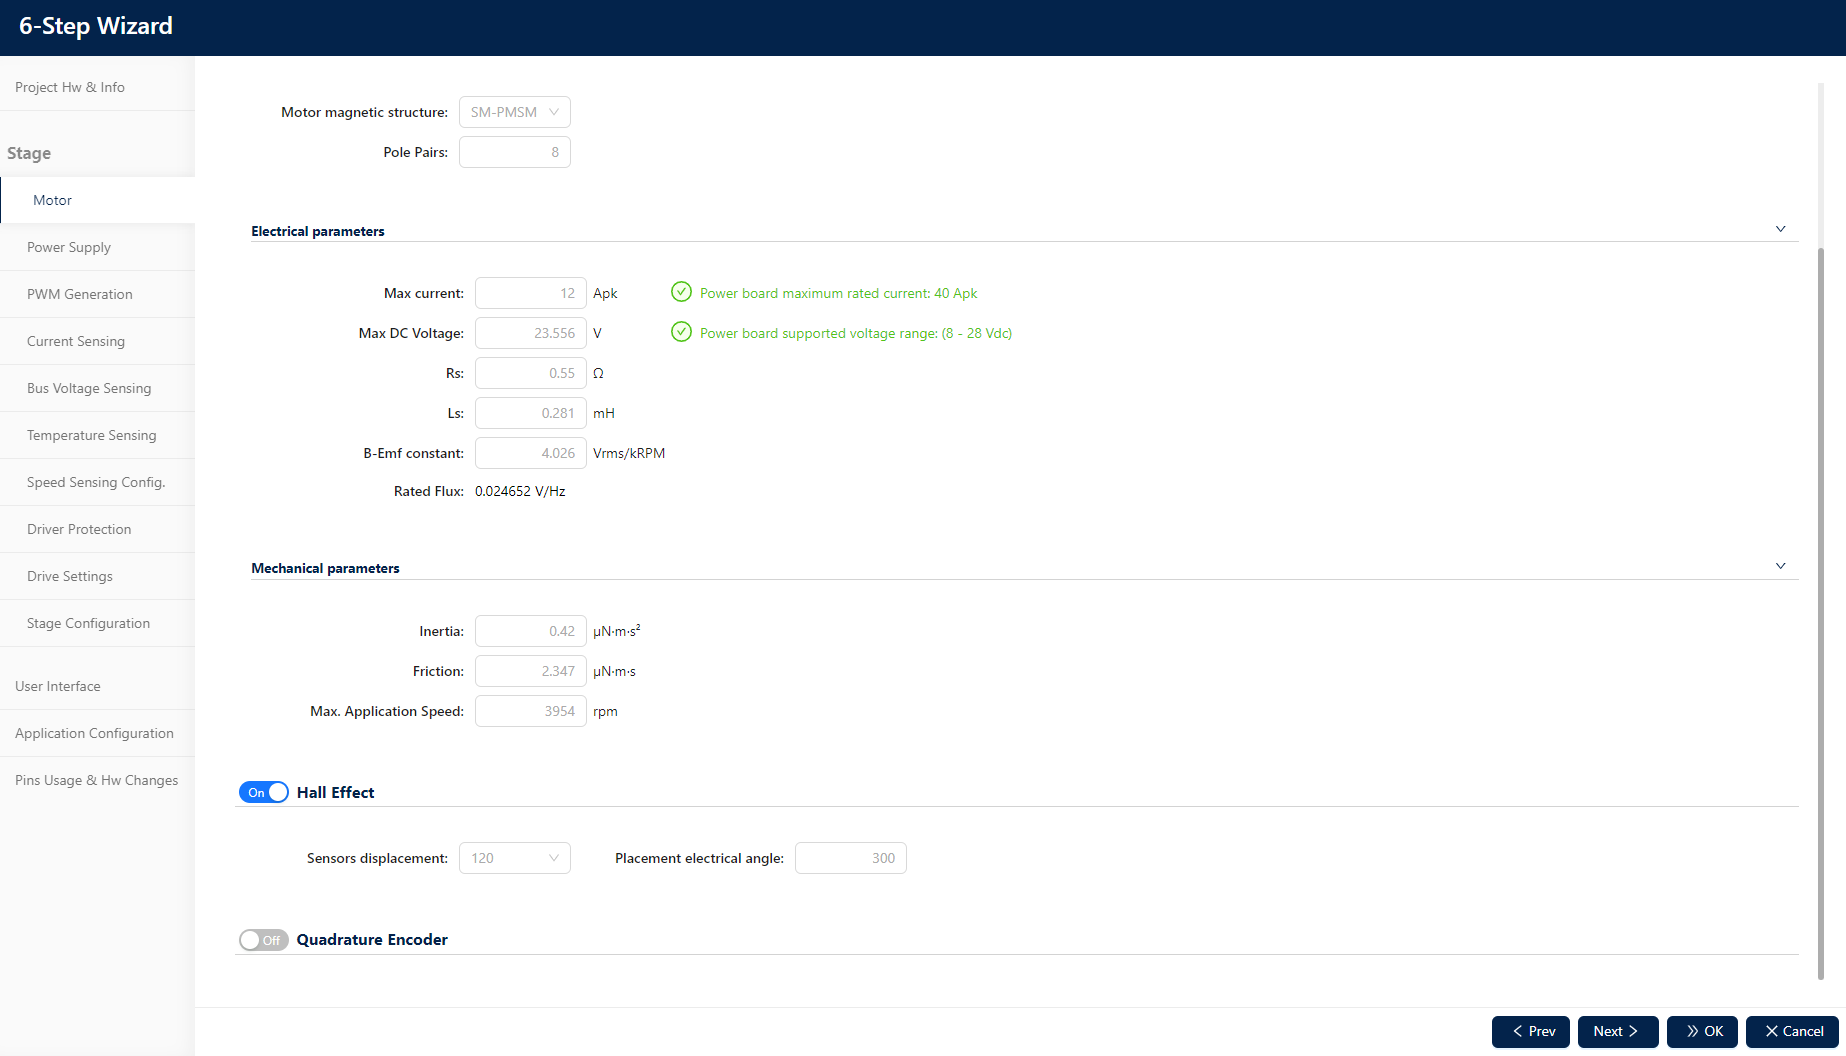
\includegraphics[width=\textwidth]{References/MCW 6-step Hall-Effect Motor.png}}
                        \caption{MotorControl Workbench Hall-Effect Select}
                    \end{figure}
                \item Select \emph{Speed Sensing Selection} and select \emph{Hall-Effect} in \emph{Speed Sensor Mode} and select \emph{OK} in the bottom right.
                    \begin{figure}[H]
                        \centerline{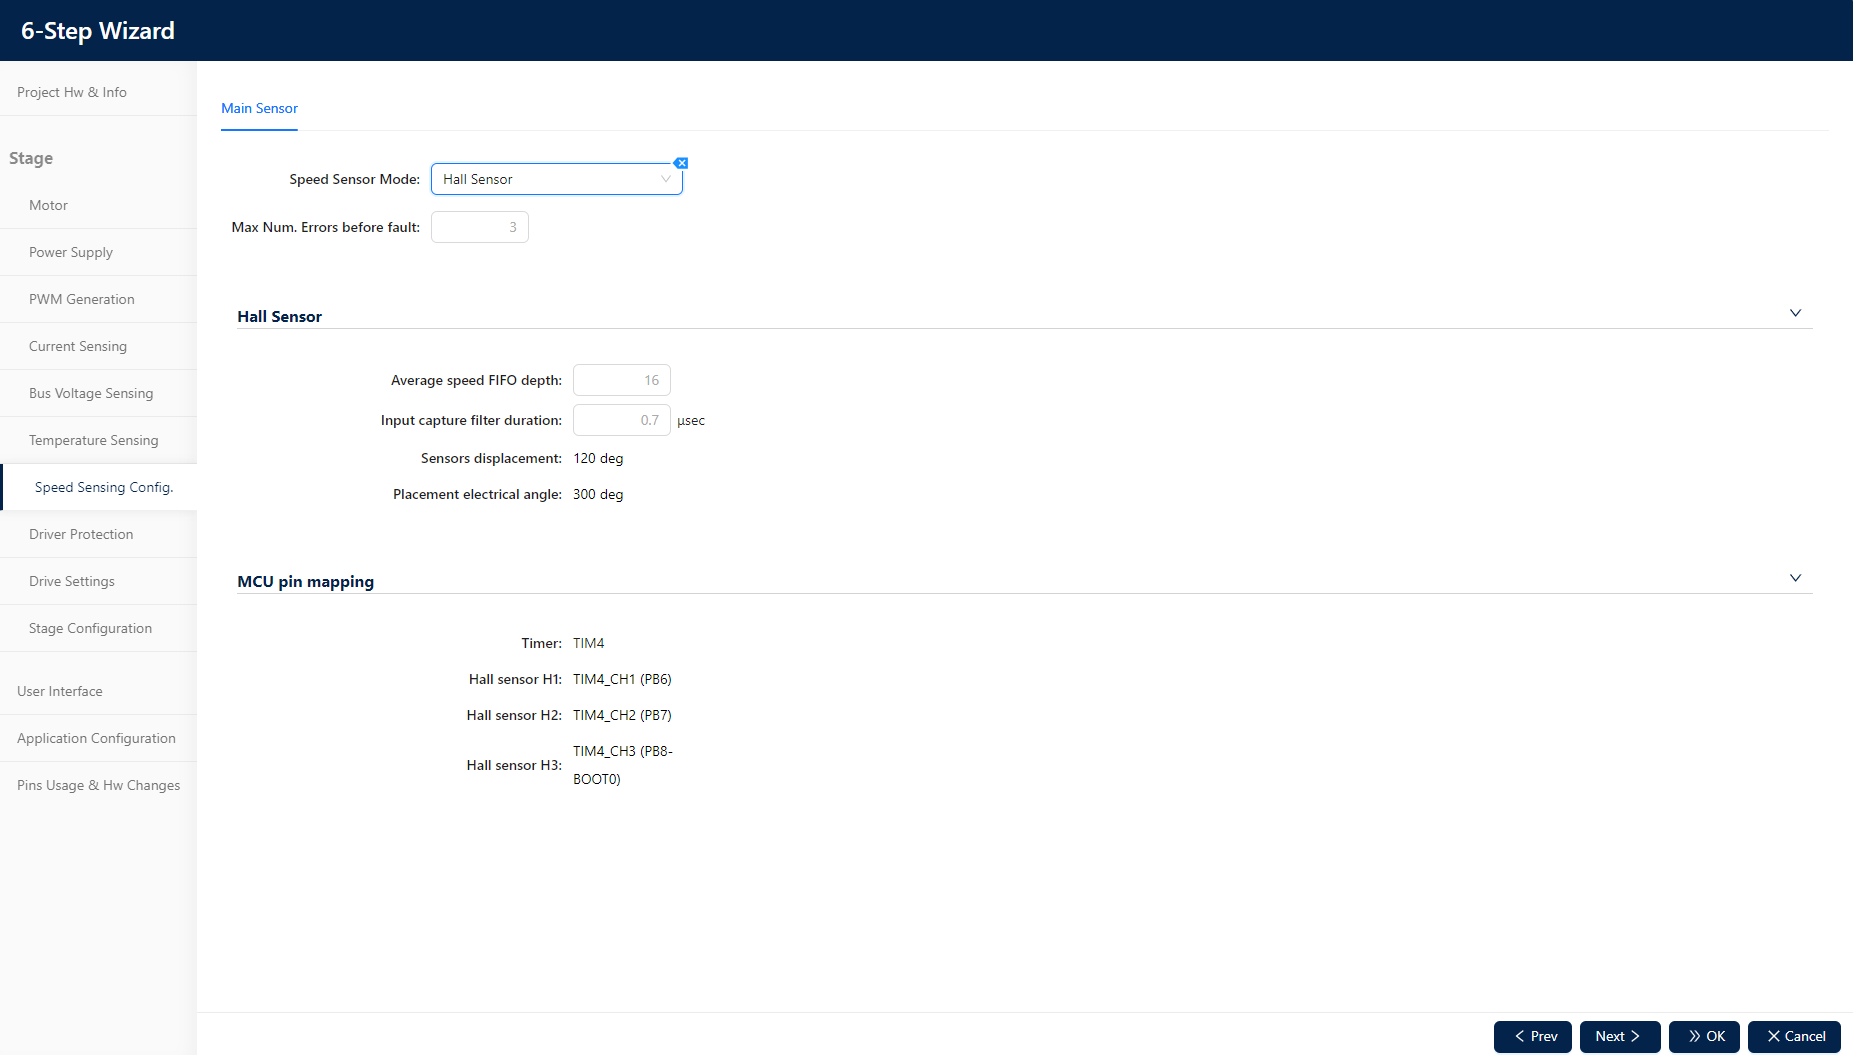
\includegraphics[width=\textwidth]{References/MCW 6-step Speed Sensing Selection.png}}
                        \caption{MotorControl Workbench Speed Sensing Selection}
                    \end{figure}
                \item Click \emph{Generate the project} at the top of the screen and save it.
                    \begin{figure}[H]
                        \centerline{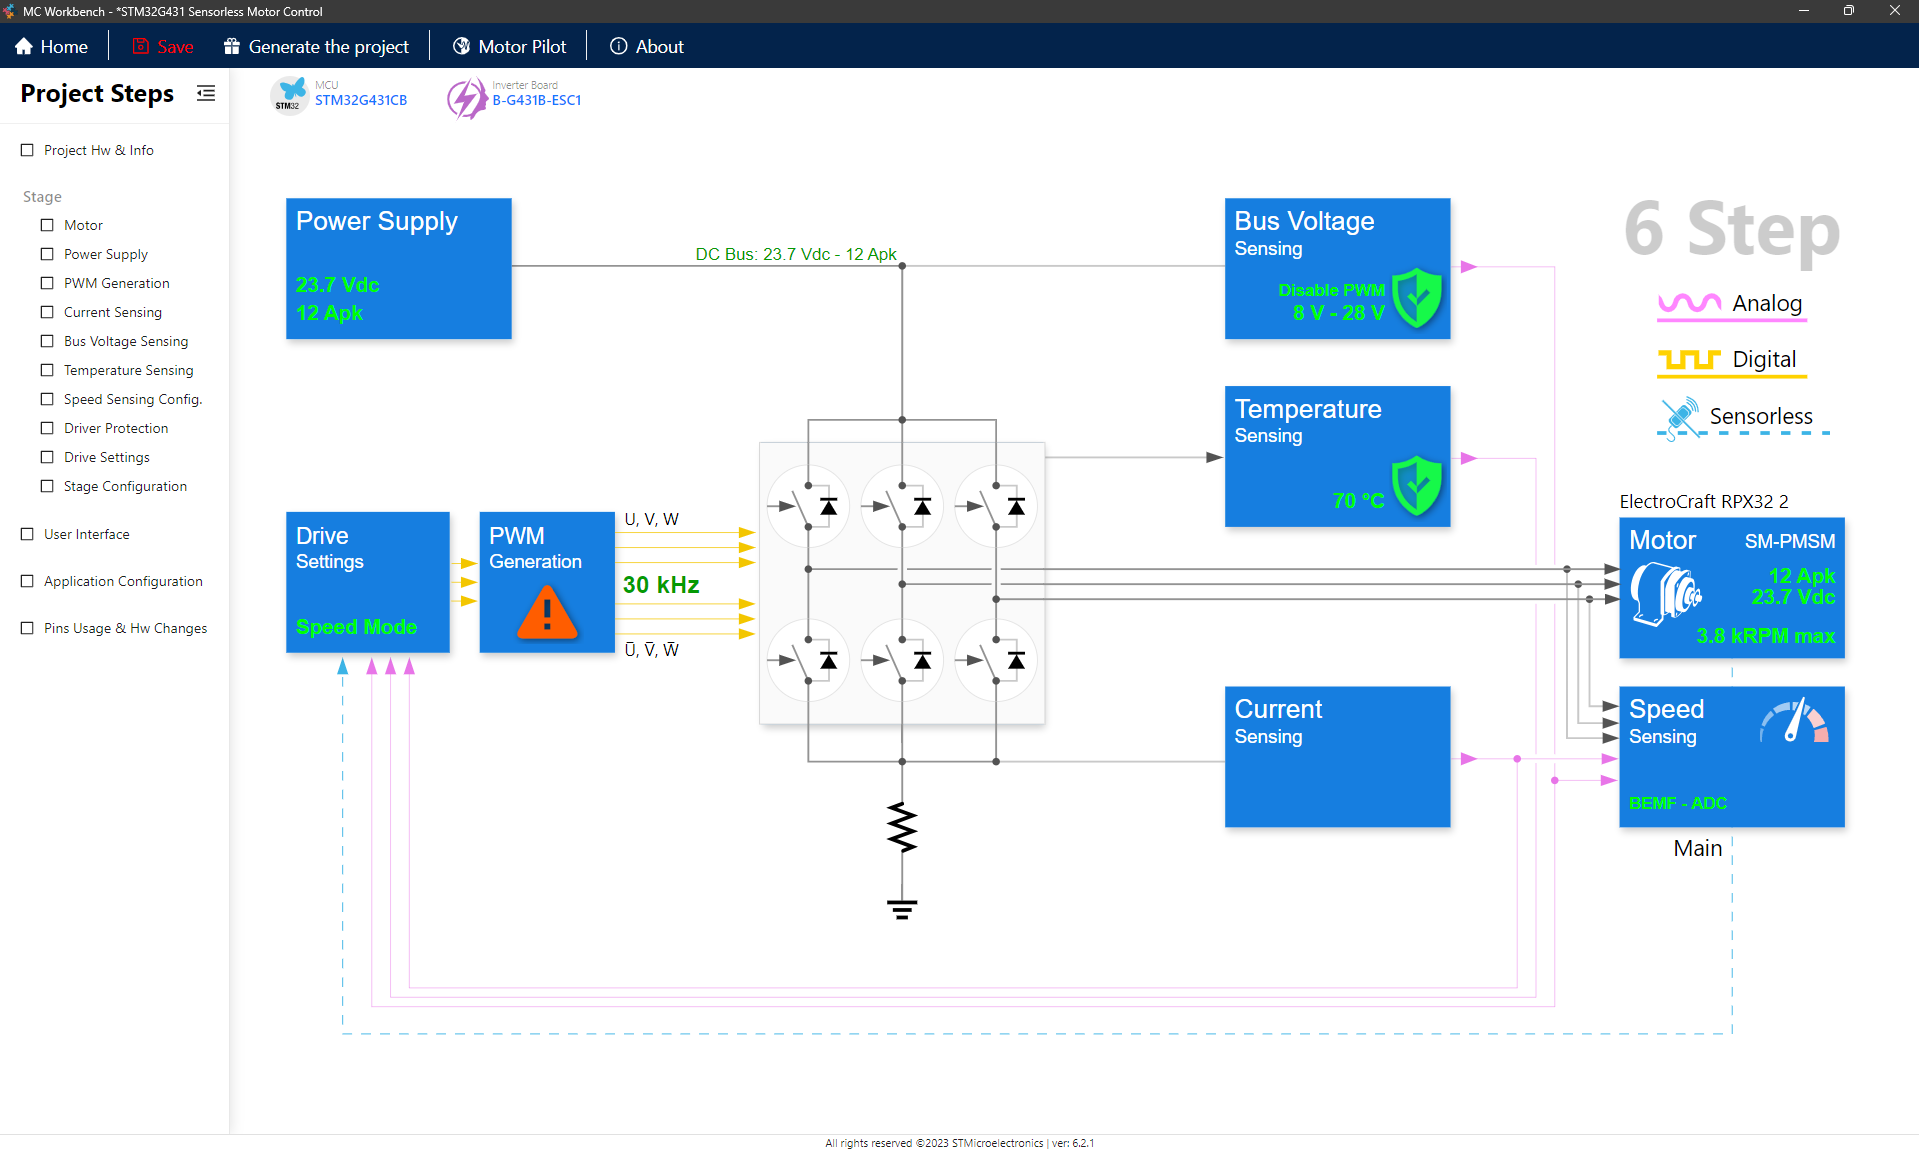
\includegraphics[width=\textwidth]{References/MCW Project Screen.png}}
                        \caption{MotorControl Workbench Project Screen}
                    \end{figure}
                \item Next the \emph{Project generation} screen will appear. Select the latest version of STM32CubeMX as your \emph{STM32CubeMX} version, select \emph{IAR EWARM V8} as your \emph{Target Toolchain}, and leave the recommended firmware under \emph{Firmware Package Version} and \emph{HAL - Hardware Abstraction Layer} as \emph{Drive Type}.
                    \begin{figure}[H]
                        \centerline{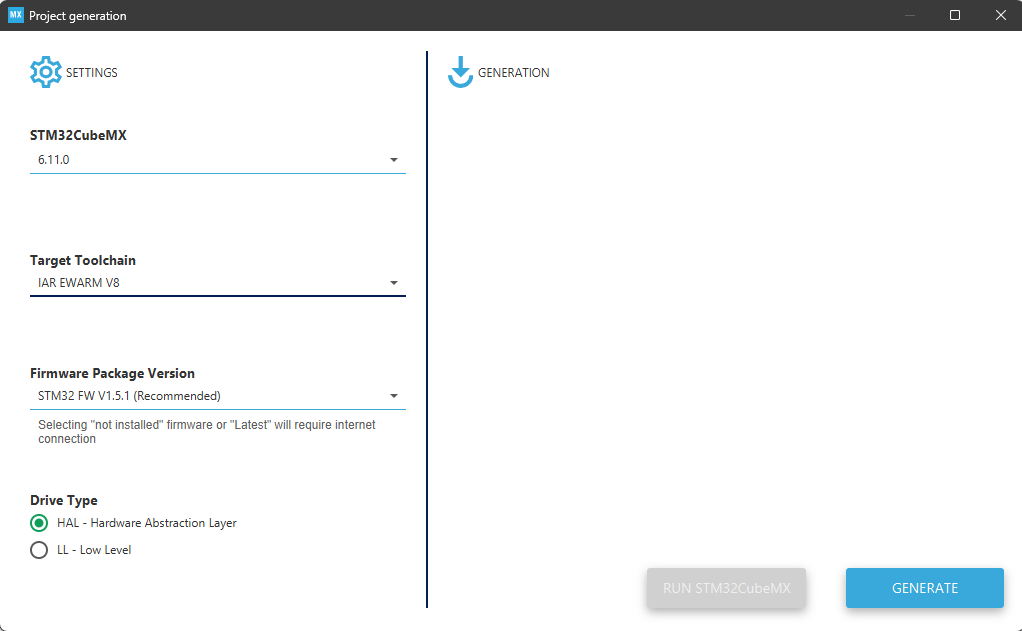
\includegraphics[width=\textwidth]{References/MCW Project Gen.png}}
                        \caption{MotorControl Workbench Project Generation Screen}
                    \end{figure}
                \item Select \emph{GENERATE}. It may ask you to install firmware, do so if prompted.
                \item Once completed, select \emph{RUN STM32CubeMX}.
            \end{itemize}
		\FloatBarrier \subsection{STM32CubeMX}
            The only thing required to do in STM32CubeMX is click \emph{GENERATE CODE} in the top right and then \emph{Open Project} when completed. You may be tempted to skip this step is subsequent runs as MotorControl Workbench will automatically regenerate some code, but if anything involving the ports needs to be updated, STM32CubeMX will need to be run.
            \begin{figure}[H]
                \centerline{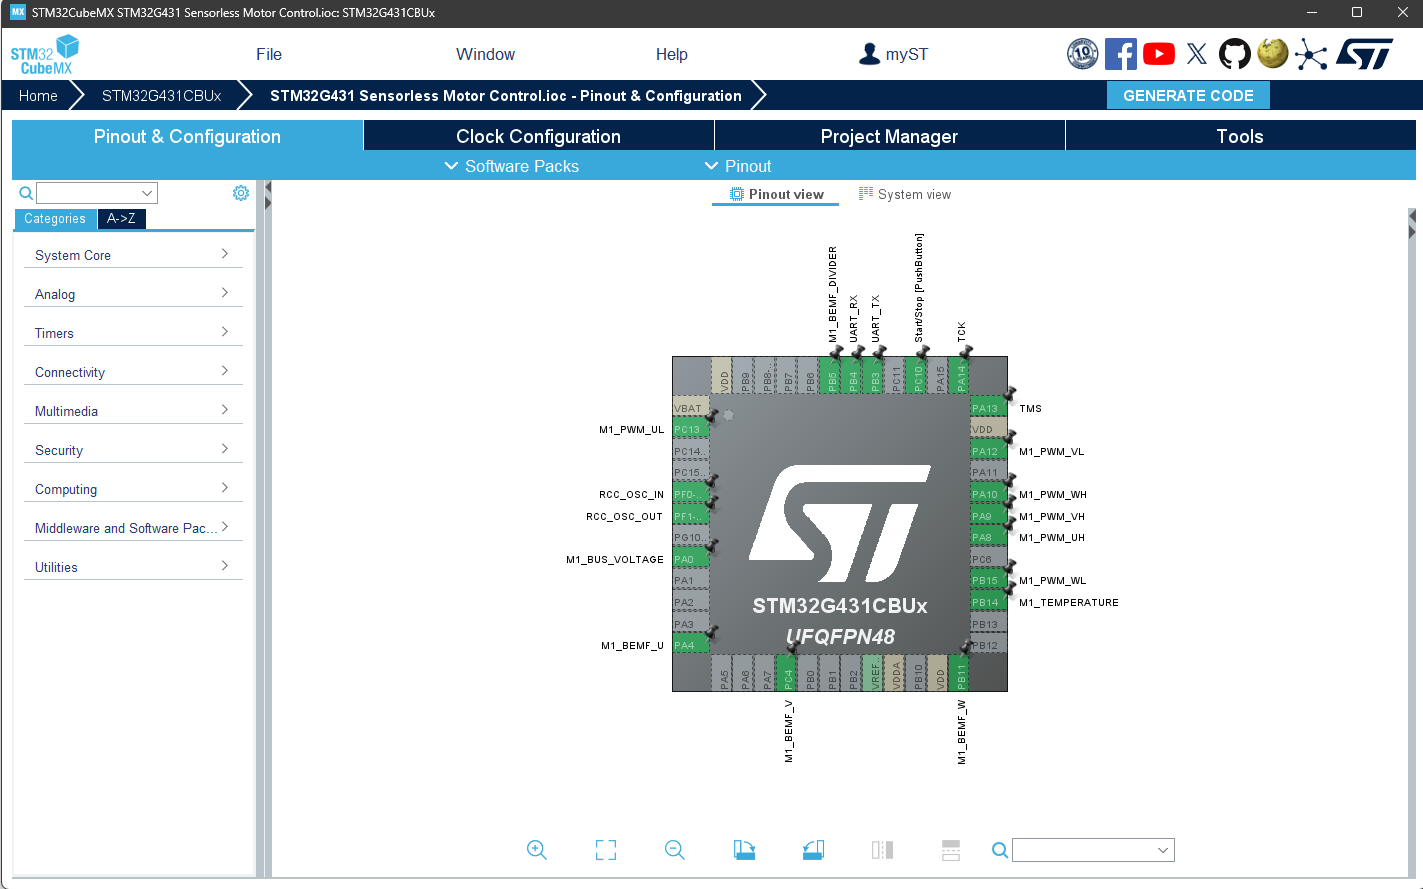
\includegraphics[width=\textwidth]{References/CubeMX.png}}
                \caption{STM32CubeMX Project Screen}
                    \end{figure}
		\FloatBarrier \subsection{IAR EW for ARM}
                    A screen will pop up asking if you would like to upgrade the project to the latest IAR version. Do so. You can compile and download the project to the board in IAR using the green button with a white triangle. You can turn on and off the motor using the button on the control board.
			\FloatBarrier \subsubsection{Motor Functions}
                        There are three main functions used in the operation of the motor in this section.
                        \begin{enumerate}
                            \item \texttt{MC\_StartMotor1(void)} - Starts the motor.
                            \item \texttt{MC\_StopMotor1(void)} - Stops the motor
                            \item \texttt{MC\_ProgramSpeedRampMotor1\_F(float\_t FinalSpeed, uint16\_t hDurationms)} - Select motor rotation speed. \texttt{FinalSpeed} is in RPM, the sign of this number is the rotation direction. \texttt{hDurationms} is number of milliseconds it will take the motor to reach this speed. 0 is follow mode which I have found to not be very accurate, the minimum I would set this is 20 ms.
                        \end{enumerate}
			\FloatBarrier \subsubsection{While Loop Motor Operation}
                    \textbf{Commit} - 572c949218ae4c62735c8cc8e073d14ff63f6cde \\
                When code is generated by the MotorControl Workbench or STM32CubeMX, there will be \texttt{/* USER CODE */} around sections that will survive from one generation to the next. Additionally we can use the function \texttt{HAL\_Delay(delay\_ms)} to insert a delay between operations. Therefore the code 
                \begin{verbatim}
while (1)
{
    /* USER CODE END WHILE */

    /* USER CODE BEGIN 3 */
    MC_StartMotor1();
    HAL_Delay(2000);
    MC_StopMotor1();
    HAL_Delay(400);
}
                \end{verbatim}
                will start the motor, delay by 2000 ms (2 seconds), stop the motor, delay by 400 ms, then loop back to the top. \\ 
                You should always set a speed before stating the motor for the first time. In the section labeled \texttt{/* USER CODE BEGIN 2 */}, insert
                \begin{verbatim}
/* USER CODE BEGIN 2 */
MC_ProgramSpeedRampMotor1_F(1500, 1000);

/* USER CODE END 2 */
                \end{verbatim}
                This will set the motor to 1500 RPM after a 1000 ms (1 second) ramp up period. You can now compile, download, and run this code on your board. You will need to hit the white circle with blue arrow in it at the top of IAR to run the code. \\ 
                \textbf{Commit} - 646d2fe1c341b52f06541492c38e549af42f2f65 \\
                A more interesting way to run the motor is to reverse its direction after ever start/stop. To do this, we can insert the\texttt{ MC\_ProgramSpeedRampMotor1} function after each stop, with a negative rotation every other start/stop.
                \begin{verbatim}
while (1)
{
    /* USER CODE END WHILE */

    /* USER CODE BEGIN 3 */
    MC_StartMotor1();
    HAL_Delay(2000);
    MC_StopMotor1();
    HAL_Delay(400);
    MC_ProgramSpeedRampMotor1_F(-1500, 1000);
    MC_StartMotor1();
    HAL_Delay(2000);
    MC_StopMotor1();
    HAL_Delay(400);
    MC_ProgramSpeedRampMotor1_F(1500, 1000);
}
                \end{verbatim}
                This will start the motor going the forward direction (because of the code in \texttt{/* USER CODE END 2 */}) then after it stops, start it going the other direction. It will then repeat. Mess around with the RPM and ramp up time to get a sense of how to use the motor. \emph{NOTE} I have empirically discovered that you need a 400 ms delay between stopping and starting the motor to get it to change direction. This is because the motor need to be in IDLE before it will change direction.
			\FloatBarrier \subsubsection{Button Motor Operation}
                    \textbf{Commit} - f1e3a17f54fe1d8a11798c82724a993aac265f93 \\
                    By default, the MotorControl Workbench projects will default to starting and stopping motor with button press. You can try this out with the main loop, but your control will be overwritten quickly by the while loop. To change this, we can remove the code in the while loop and move parts of it further up the main function to where the previous speed initialization was. The code below will run the motor for 2 seconds and then stop it. Afterward, you are free to control the motor with the button on the board.
                    \begin{verbatim}
/* USER CODE BEGIN 2 */
MC_ProgramSpeedRampMotor1_F(1500, 1000);
MC_StartMotor1();
HAL_Delay(2000);
MC_StopMotor1();

/* USER CODE END 2 */
                    \end{verbatim}
                    Build, download, run, and test this. \\
                    You will notice that the motor does not reverse direction. To do this, we need to go into the \texttt{UI\_HandleStartStopButton\_cb} function in \texttt{mc\_tasks.c}. We need a variable to keep track to the previous direction and a control statement to decide which direction the motor should be running. Since we start motor in forward direction, we should reverse direction on first pass.
                    \begin{verbatim}
__weak void UI_HandleStartStopButton_cb (void)
{
/* USER CODE BEGIN START_STOP_BTN */
    static bool direction = 0;
  if (IDLE == MC_GetSTMStateMotor1())
  {
    /* Ramp parameters should be tuned for the actual motor */
    if (direction == 0)
    {
        MC_ProgramSpeedRampMotor1_F(-1500, 1000);
        direction = 1;
    }
    else
    {
        MC_ProgramSpeedRampMotor1_F(1500, 1000);
        direction = 0;
    }

    (void)MC_StartMotor1();
  }
  else
  {
    (void)MC_StopMotor1();
  }
/* USER CODE END START_STOP_BTN */
}
                    \end{verbatim}
                    Build, run, and test this code. This allows you to be in control of what direction the motor is running and how long it is running for, great for testing the motor in a real world scenario.
	\FloatBarrier \section{Getting FOC Motor Working}
        Previously we have been using the 6-step motor algorithm. This essentially turns on and off the different motor phases to get the motor to rotate. While this works and is simple, it is not the most efficient way to do things. FOC (Field-Oriented Control) changes the magnitudes of the phase vectors in order to keep the stator orthogonal to the rotor. Essentially, it keeps the motor at its most efficient torque by keeping the magnetic pull 90 degrees ahead. Using the FOC algorithm also allows us to use torque and position to control the motor.\\
        Much of the below section is a copy paste of the \emph{Getting Sensorless Motor Working} section. The only different aspects are the wiring required, the MotorControl Workbench configuration, IAR using torque control, and the git branch. But the user added code itself is the same.
		\FloatBarrier \subsection{GIT Code}
            To make working in this document easier, my versions of the below examples will be included in a git repository that you can download. You do not need to complete this step, but it may be useful for comparing your project to a completed one. \\
            \textbf{Branch} - FOC-MotorControl
		\FloatBarrier \subsection{MotorControl Workbench}
            \textbf{Commit} - e5b65643ab28d4f42a08ae3afa63e73990606f1c \\
            \begin{itemize}
                \item Open MotorControl Workbench (the latest version you have). 
                    \begin{figure}[H]
                        \centerline{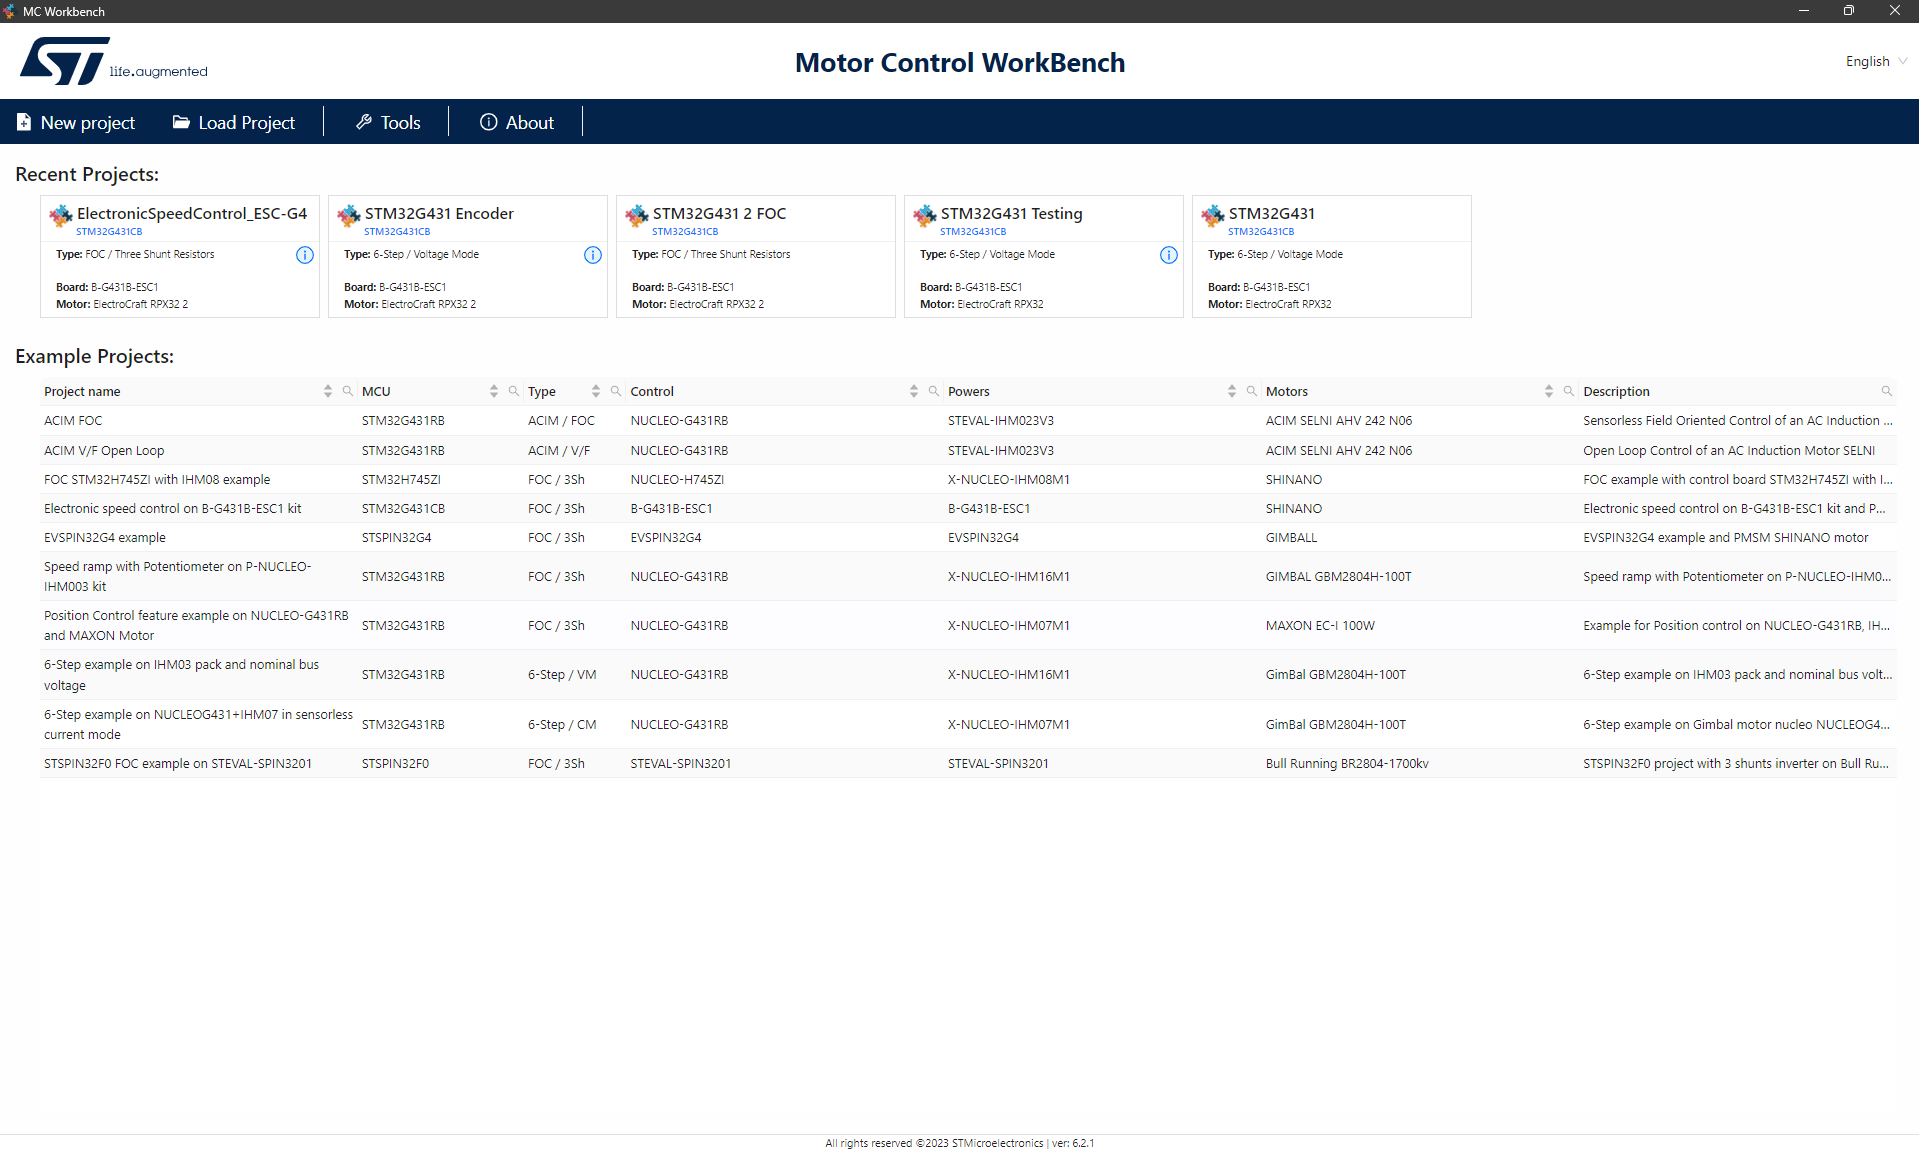
\includegraphics[width=\textwidth]{References/MC Workbench.png}}
                        \caption{MotorControl Workbench}
                    \end{figure}
                \item Select \emph{New project} in the top left.
                \item Give your project a name like "STM32G431 FOC Motor Control"
                \item \emph{Num. Motors} is 1 Motor, \emph{Driving Algorithm} is FOC, and \emph{Hardware Mode} is Inverter. Click Next at the bottom right.
                    \begin{figure}[H]
                        \centerline{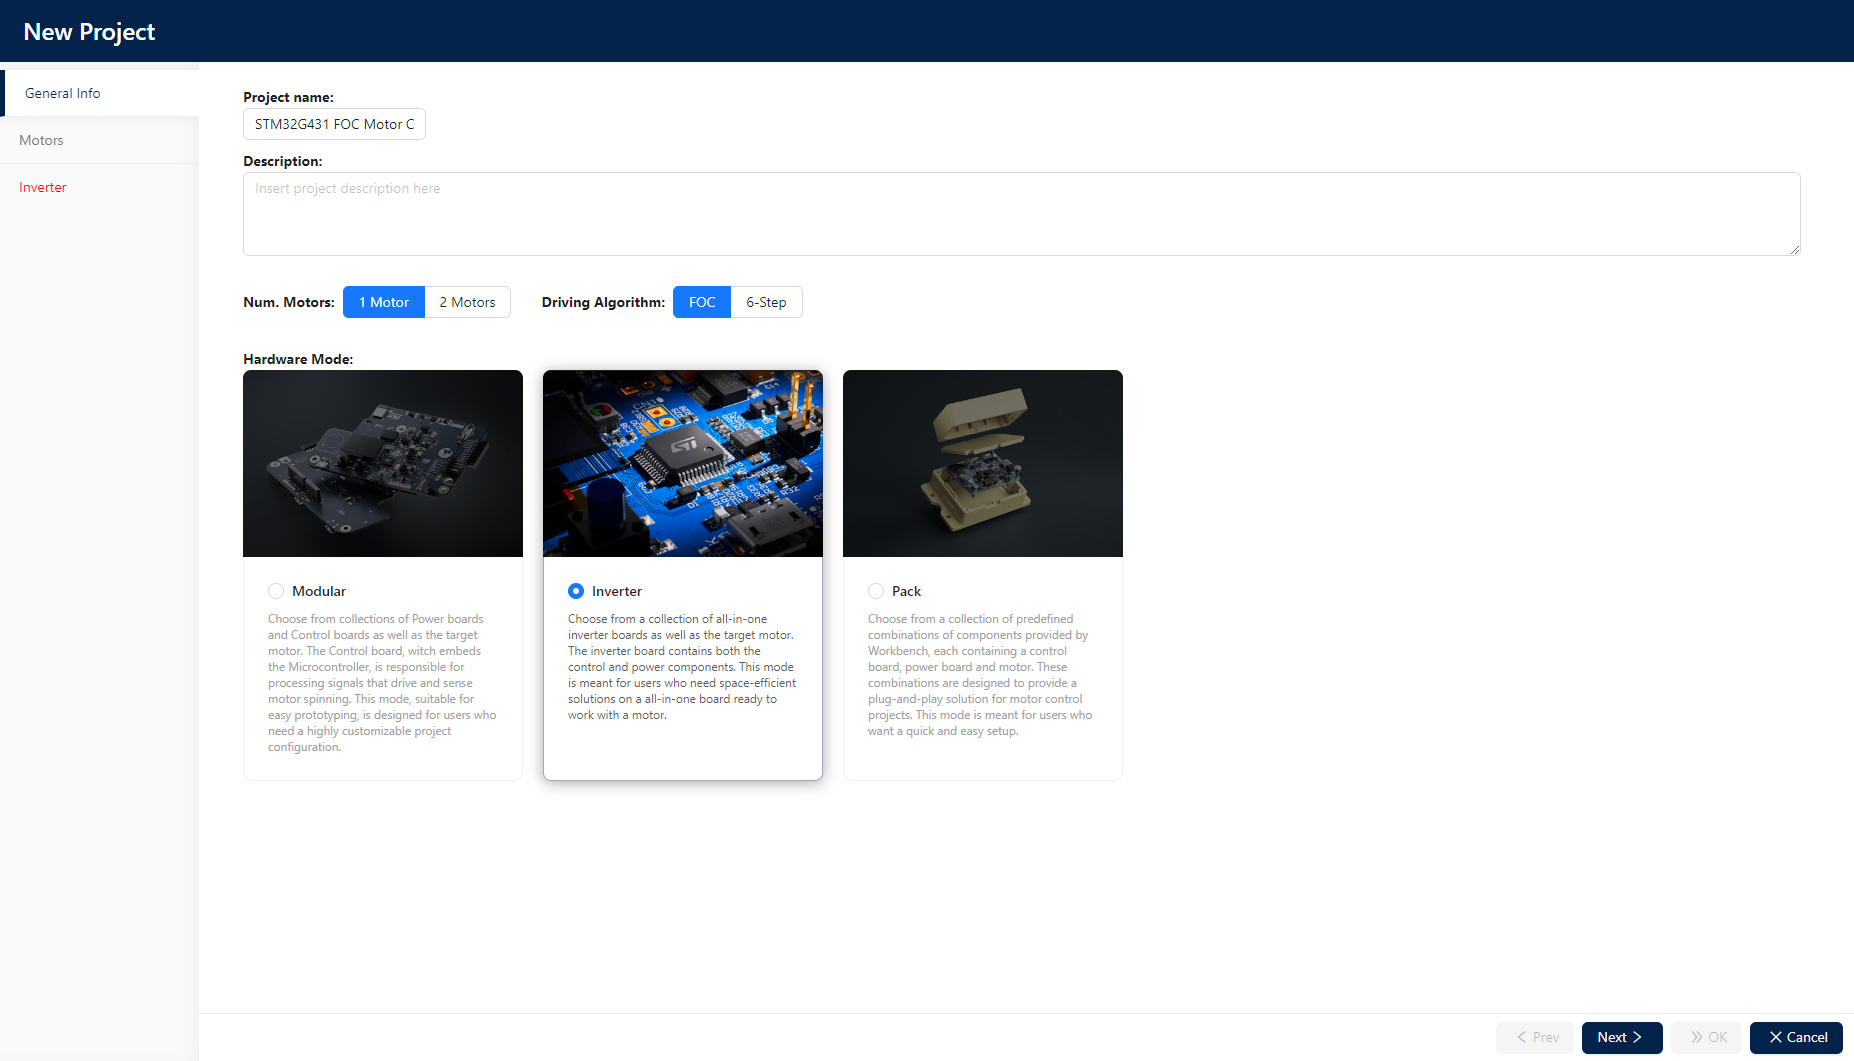
\includegraphics[width=\textwidth]{References/MCW FOC New Project.png}}
                        \caption{MotorControl Workbench New Project}
                    \end{figure}
                \item Select the Motor you profiled in the previous section. Click Next
                \item Select B-G431B-ESC1 as your board. Click OK.
                \item This will bring you to the MotorControl Workbench Project screen.
                    \begin{figure}[H]
                        \centerline{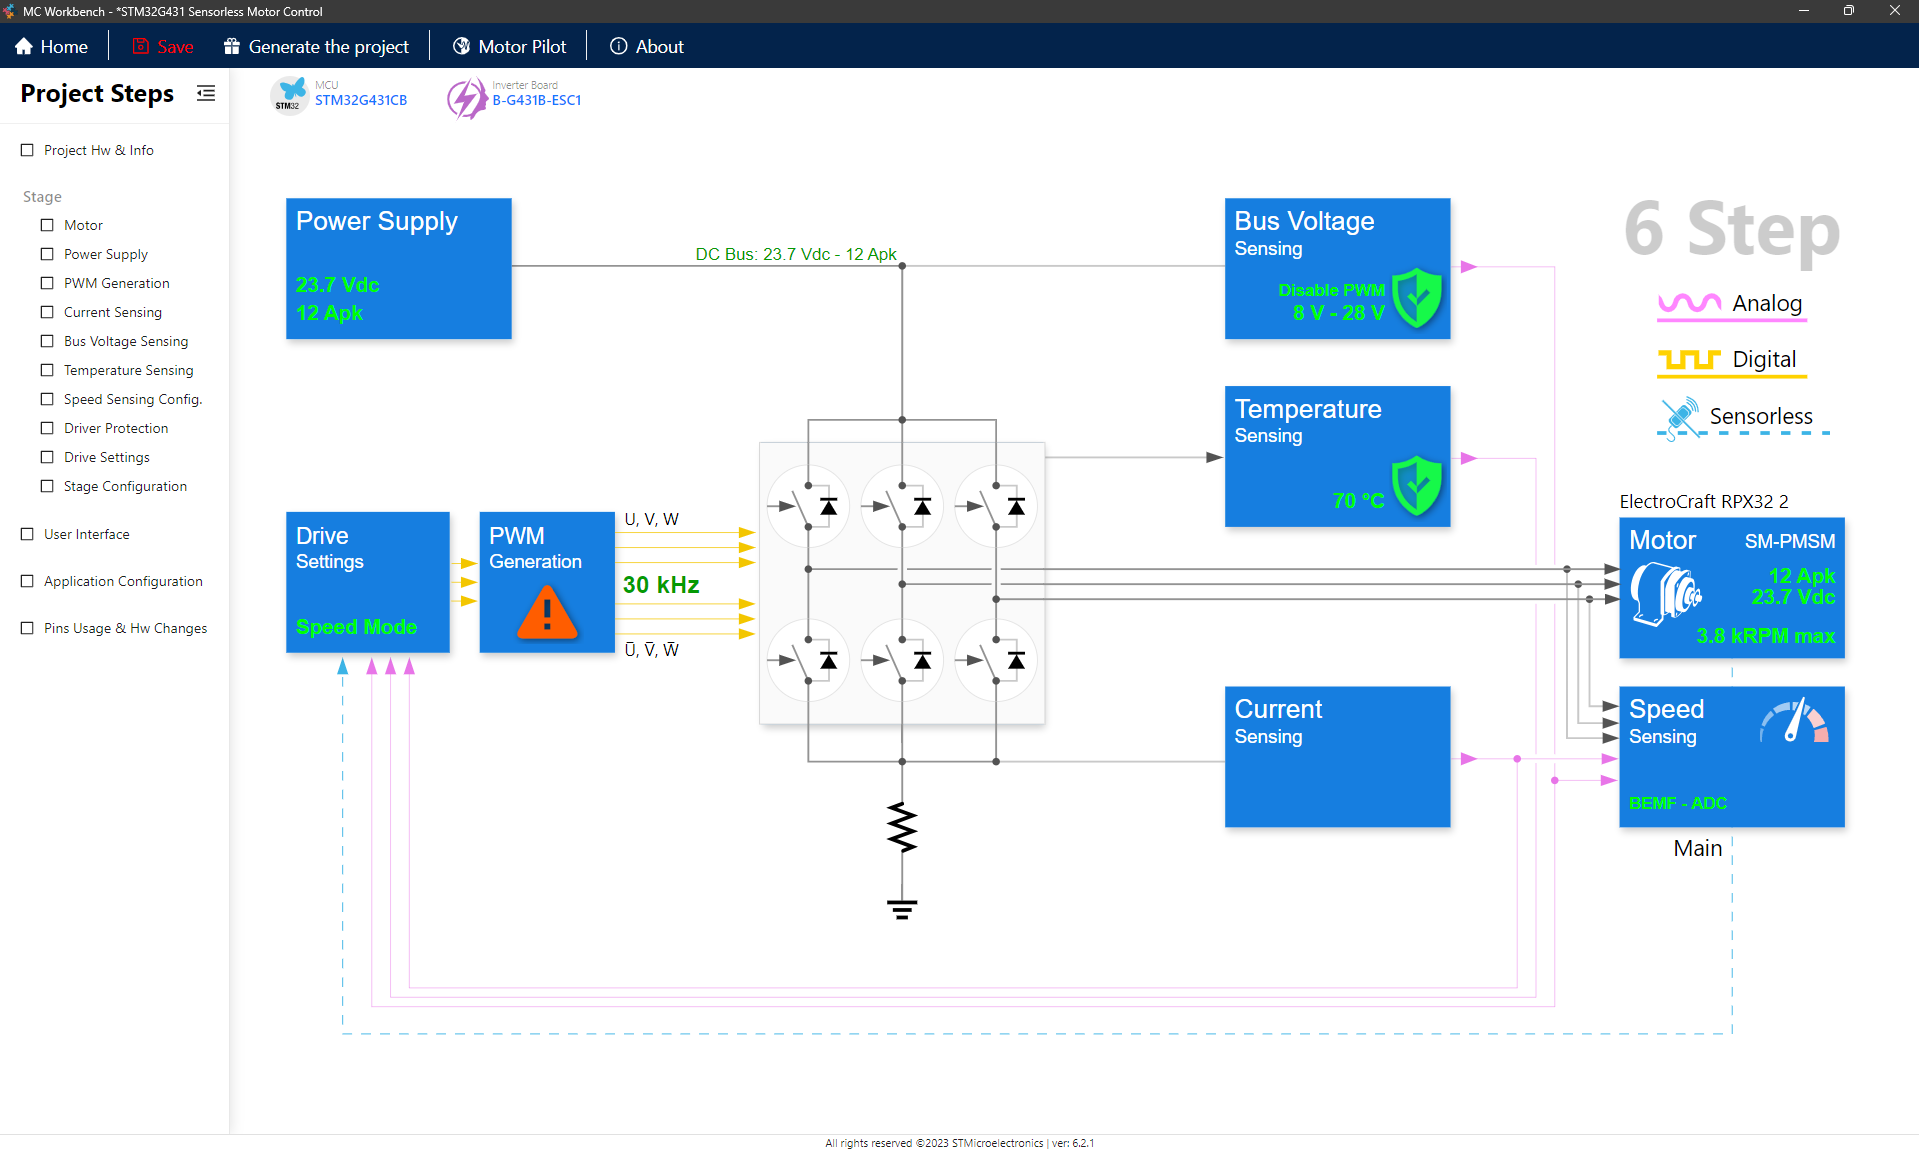
\includegraphics[width=\textwidth]{References/MCW Project Screen.png}}
                        \caption{MotorControl Workbench Project Screen}
                    \end{figure}
                \item From here, either click on \emph{Motor} on the left hand side or click the motor on the right hand side. Scroll down on this page to where is says \emph{Hall Effect} and turn this on and make sure \emph{Sensor displacement} is set to 120.
                    \begin{figure}[H]
                        \centerline{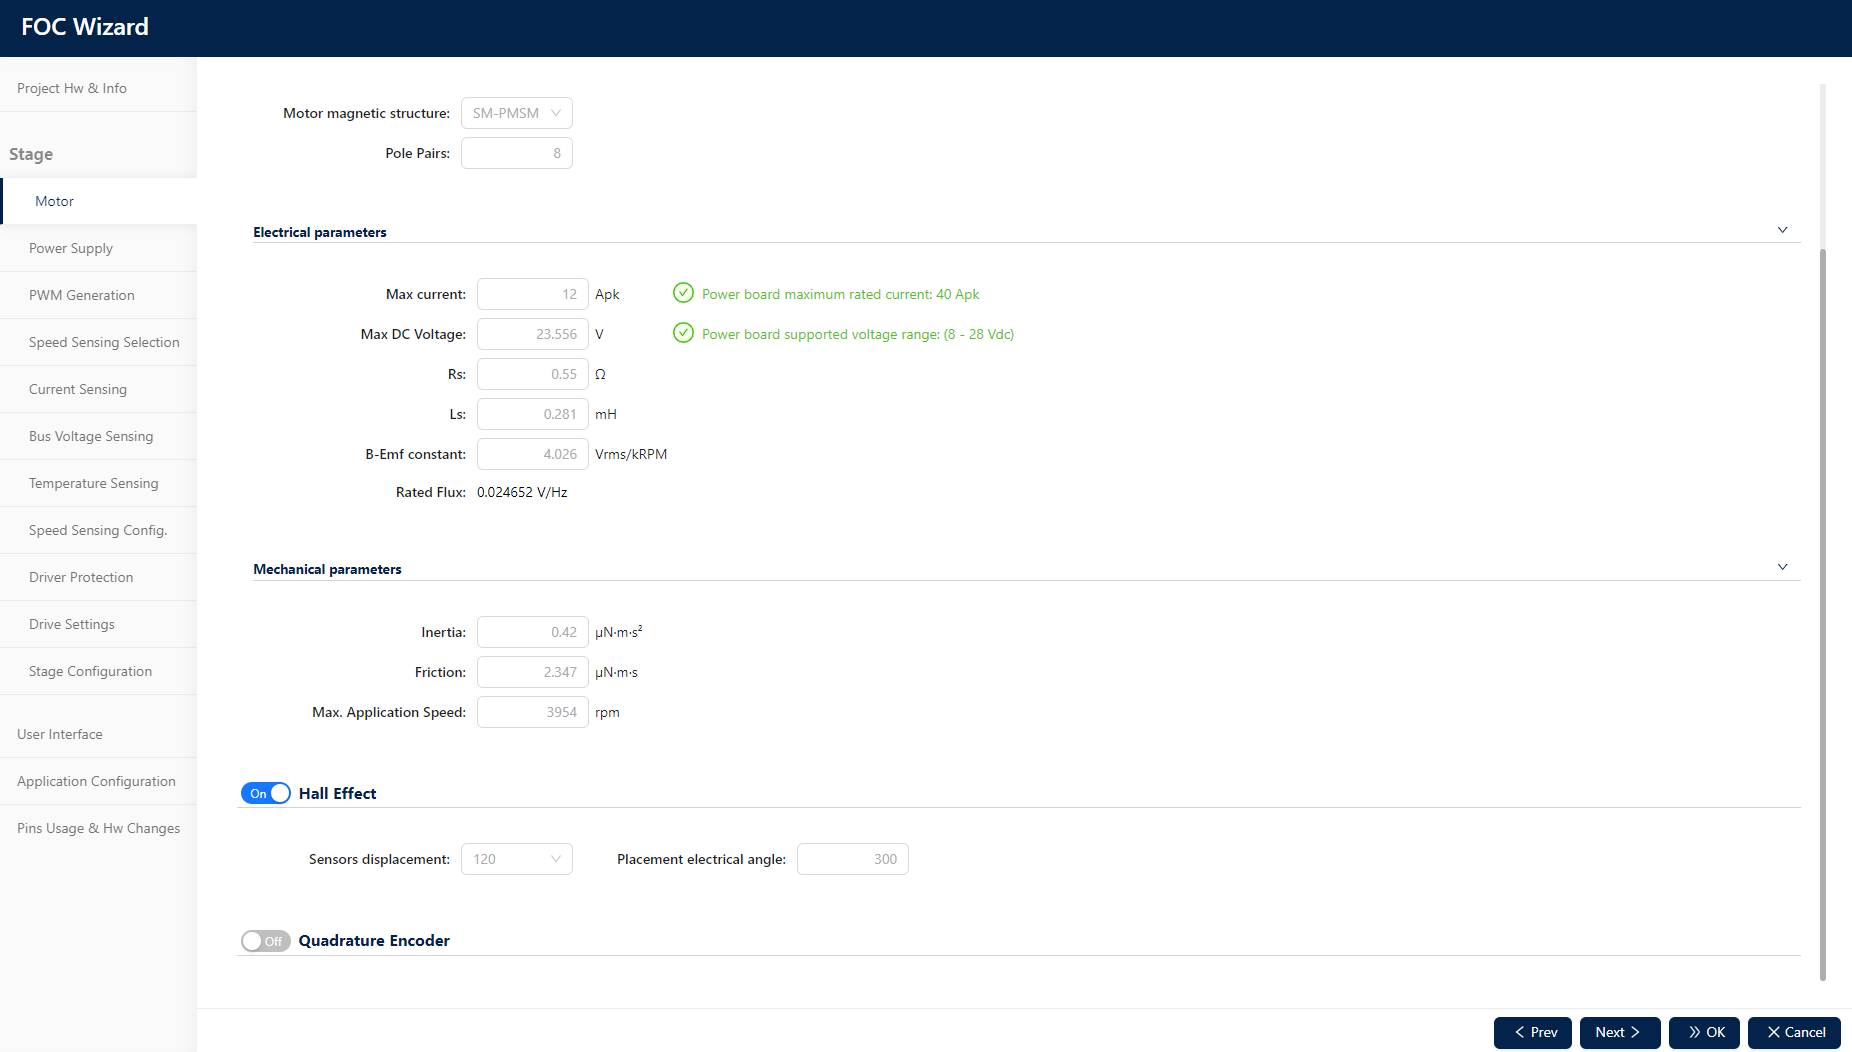
\includegraphics[width=\textwidth]{References/MCW FOC Hall-Effect Motor.png}}
                        \caption{MotorControl Workbench Hall-Effect Select}
                    \end{figure}
                \item Select \emph{Speed Sensing Selection} and select \emph{Hall-Effect} in \emph{Speed Sensor Mode}.
                    \begin{figure}[H]
                        \centerline{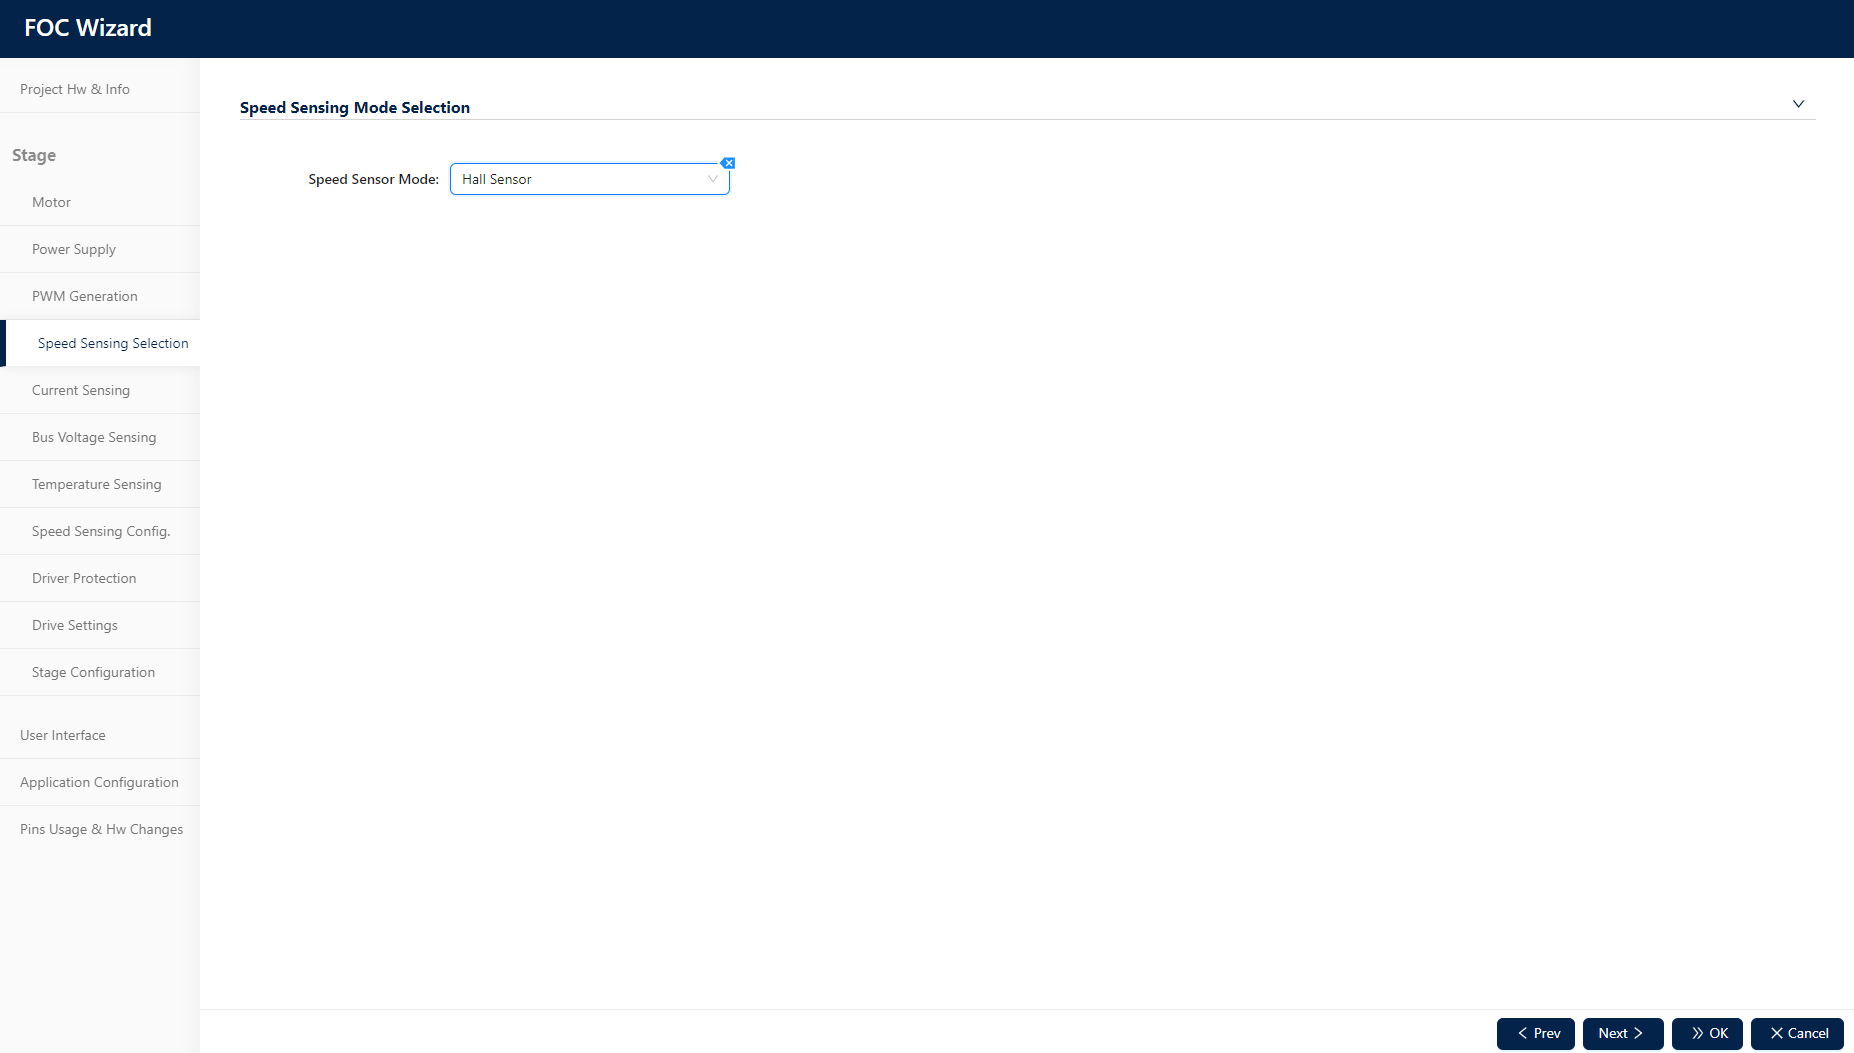
\includegraphics[width=\textwidth]{References/MCW FOC Speed Sensing Selection.png}}
                        \caption{MotorControl Workbench Speed Sensing Selection}
                    \end{figure}
                \item Finally, select \emph{Drive Settings} and select \emph{Torque control} in \emph{Control mode} and select \emph{OK} in the bottom right.
                    \begin{figure}[H]
                        \centerline{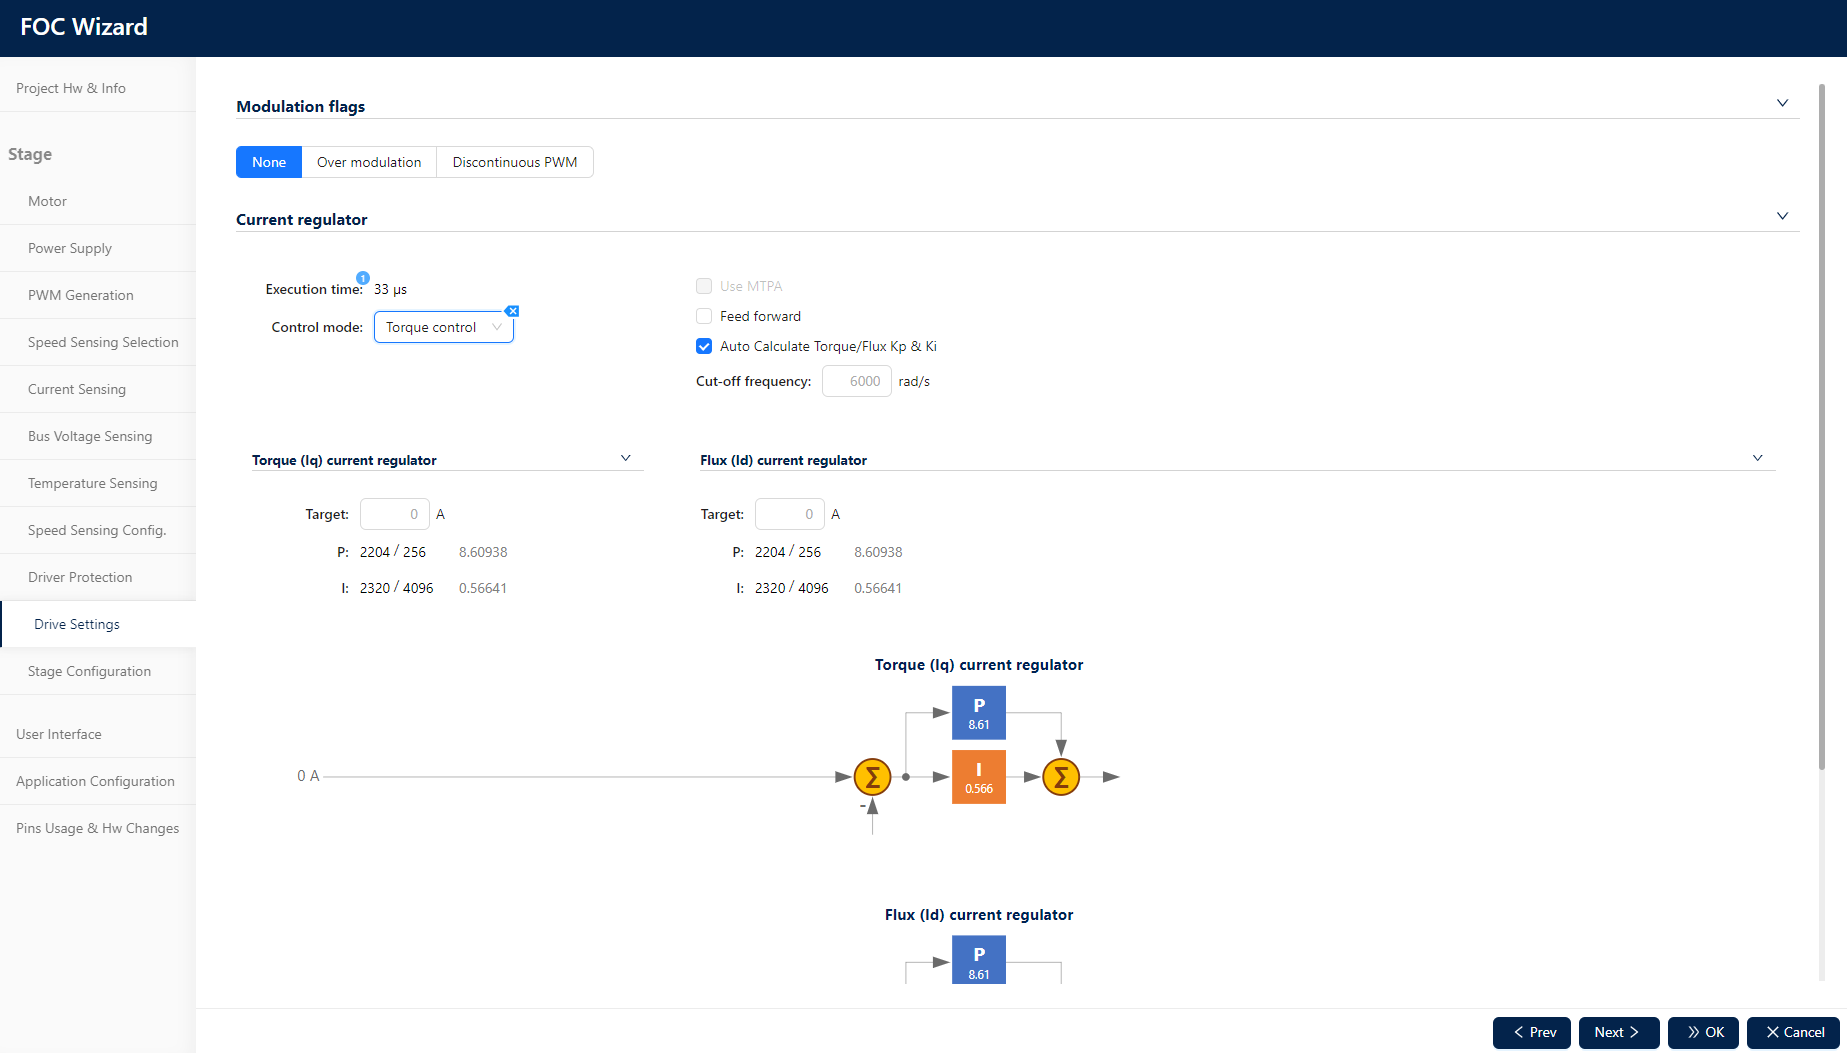
\includegraphics[width=\textwidth]{References/MCW FOC Control Mode.png}}
                        \caption{MotorControl Workbench Control Mode}
                    \end{figure}
                \item Click \emph{Generate the project} at the top of the screen and save it.
                \item Next the \emph{Project generation} screen will appear. Select the latest version of STM32CubeMX as your \emph{STM32CubeMX} version, select \emph{IAR EWARM V8} as your \emph{Target Toolchain}, and leave the recommended firmware under \emph{Firmware Package Version} and \emph{HAL - Hardware Abstraction Layer} as \emph{Drive Type}.
                    \begin{figure}[H]
                        \centerline{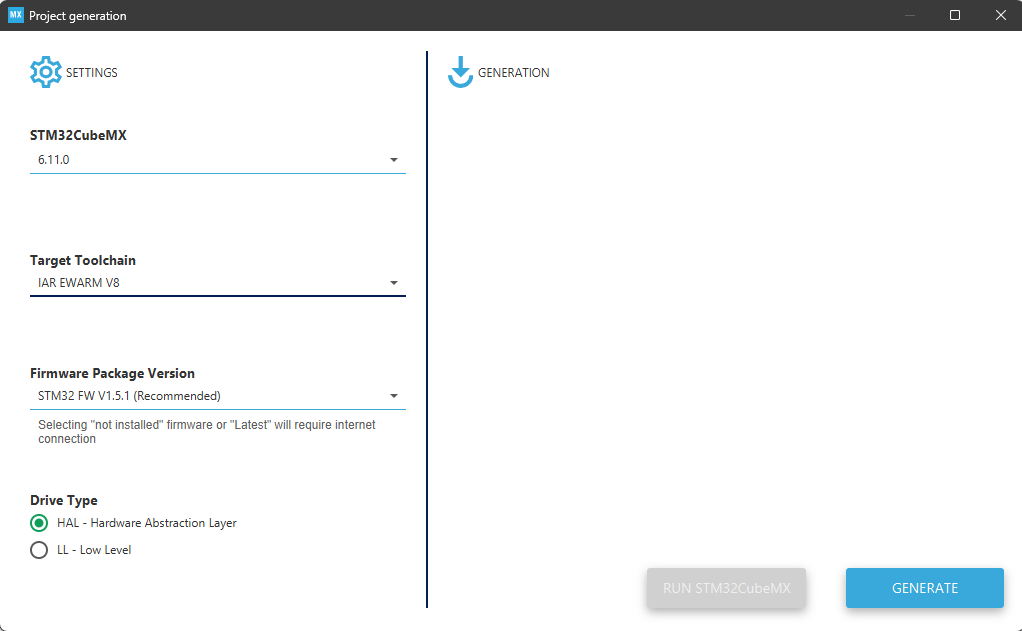
\includegraphics[width=\textwidth]{References/MCW Project Gen.png}}
                        \caption{MotorControl Workbench Project Generation Screen}
                    \end{figure}
                \item Select \emph{GENERATE}. It may ask you to install firmware, do so if prompted.
                \item Once completed, select \emph{RUN STM32CubeMX}.
            \end{itemize}
		\FloatBarrier \subsection{STM32CubeMX}
            The only thing required to do in STM32CubeMX is click \emph{GENERATE CODE} in the top right and then \emph{Open Project} when completed. You may be tempted to skip this step is subsequent runs as MotorControl Workbench will automatically regenerate some code, but if anything involving the ports needs to be updated, STM32CubeMX will need to be run.
            \begin{figure}[H]
                \centerline{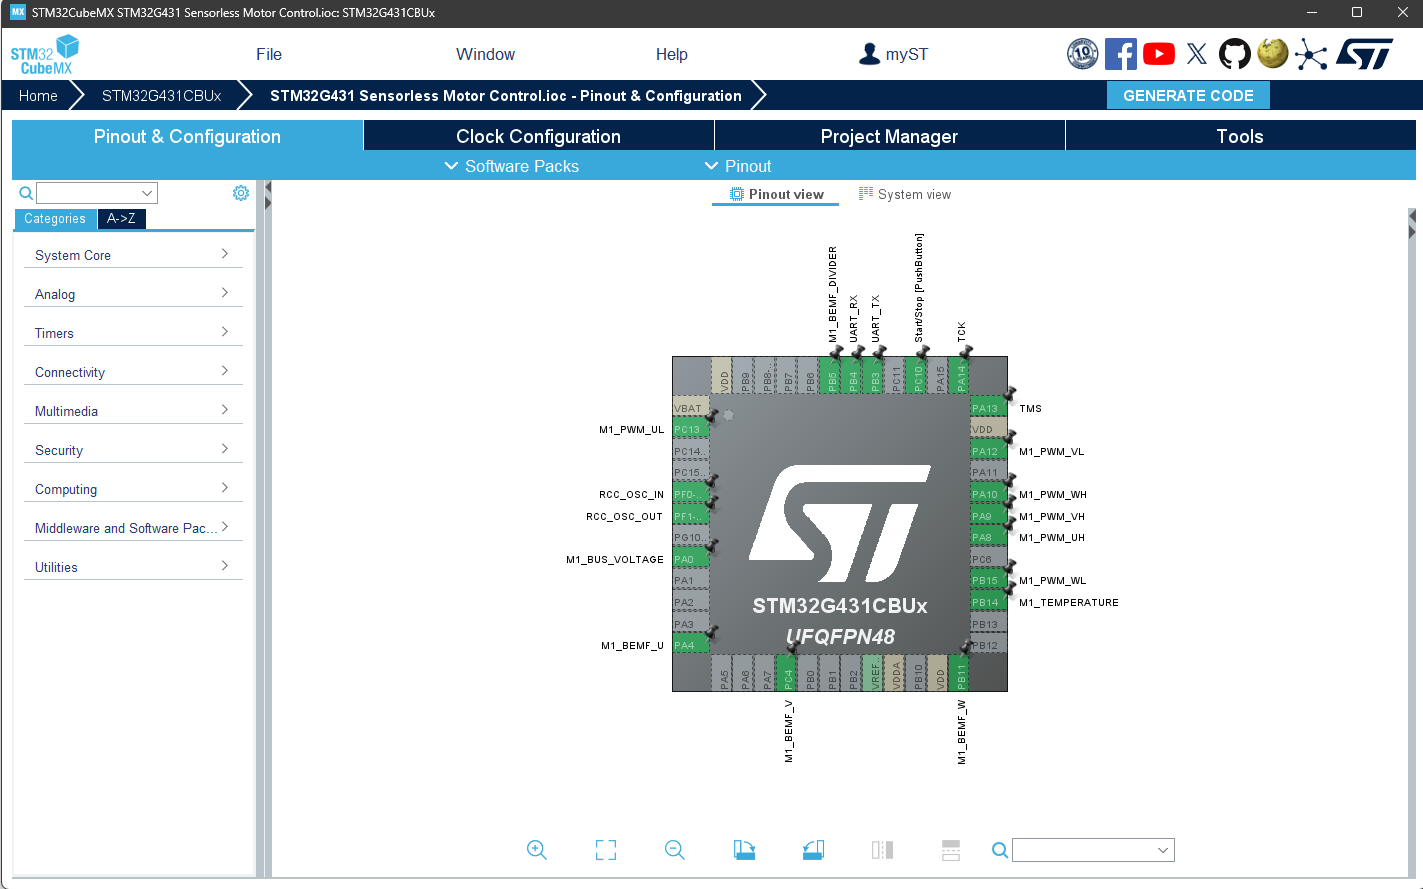
\includegraphics[width=\textwidth]{References/CubeMX.png}}
                \caption{STM32CubeMX Project Screen}
                    \end{figure}
		\FloatBarrier \subsection{IAR EW for ARM}
                    A screen will pop up asking if you would like to upgrade the project to the latest IAR version. Do so. You can compile and download the project to the board in IAR using the green button with a white triangle. You can turn on and off the motor using the button on the control board.
			\FloatBarrier \subsubsection{Motor Functions}
                        There are three main functions used in the operation of the motor in this section.
                        \begin{enumerate}
                            \item \texttt{MC\_StartMotor1(void)} - Starts the motor.
                            \item \texttt{MC\_StopMotor1(void)} - Stops the motor
                            \item \texttt{MC\_ProgramSpeedRampMotor1\_F(float\_t FinalSpeed, uint16\_t hDurationms)} - Select motor rotation speed. \texttt{FinalSpeed} is in \texttt{RPM}, the sign of this number is the rotation direction. \texttt{hDurationms} is number of milliseconds it will take the motor to reach this speed. 0 is follow mode which I have found to not be very accurate, the minimum I would set this is 20 ms.
                            \item \texttt{MC\_ProgramTorqueRampMotor1\_F(float\_t FinalTorque, uint16\_t hDurationms)} - Select motor rotation torque. \texttt{FinalTorque} is in \texttt{Amperes}, the sign of this number is the rotation direction. \texttt{hDurationms} is number of milliseconds it will take the motor to reach this speed. 0 is follow mode which I have found to not be very accurate, the minimum I would set this is 20 ms.
                        \end{enumerate}
			\FloatBarrier \subsubsection{While Loop Motor Operation}
                \textbf{Commit} - bdc75abafcff16eedec953a0aa870900cbb0b557 \\
                When code is generated by the MotorControl Workbench or STM32CubeMX, there will be \texttt{/* USER CODE */} around sections that will survive from one generation to the next. Additionally we can use the function \texttt{HAL\_Delay(delay\_ms)} to insert a delay between operations. Therefore the code 
                \begin{verbatim}
while (1)
{
    /* USER CODE END WHILE */

    /* USER CODE BEGIN 3 */
    MC_StartMotor1();
    HAL_Delay(2000);
    MC_StopMotor1();
    HAL_Delay(400);
}
                \end{verbatim}
                will start the motor, delay by 2000 ms (2 seconds), stop the motor, delay by 400 ms, then loop back to the top. \\ 
                You should always set a speed before stating the motor for the first time. In the section labeled \texttt{/* USER CODE BEGIN 2 */}, insert
                \begin{verbatim}
/* USER CODE BEGIN 2 */
MC_ProgramTorqueRampMotor1_F(1.0f, 1000);

/* USER CODE END 2 */
                \end{verbatim}
                This will set the motor torque to 1 amp after a 1000 ms (1 second) ramp up period. There is no way to limit the speed of the motor when using torque control. You can now compile, download, and run this code on your board. You will need to hit the white circle with blue arrow in it at the top of IAR to run the code. \\
                \textbf{Commit} - 3c8b6fd606cfbc1924f1a555b1ba3549a635790a \\
                A more interesting way to run the motor is to reverse its direction after ever start/stop. To do this, we can insert the \texttt{MC\_ProgramTorqueRampMotor1\_F} function after each stop, with a negative rotation every other start/stop.
                \begin{verbatim}
while (1)
{
    /* USER CODE END WHILE */

    /* USER CODE BEGIN 3 */
    MC_StartMotor1();
    HAL_Delay(2000);
    MC_StopMotor1();
    HAL_Delay(400);
    MC_ProgramTorqueRampMotor1_F(-1.0f, 1000);
    MC_StartMotor1();
    HAL_Delay(2000);
    MC_StopMotor1();
    HAL_Delay(400);
    MC_ProgramTorqueRampMotor1_F(1.0f, 1000);
}
                \end{verbatim}
                This will start the motor going the forward direction (because of the code in \texttt{/* USER CODE END 2 */}) then after it stops, start it going the other direction. It will then repeat. Mess around with the Amps and ramp up time to get a sense of how to use the motor. \emph{NOTE} I have empirically discovered that you need a 400 ms delay between stopping and starting the motor to get it to change direction. This is because the motor need to be in IDLE before it will change direction.
			\FloatBarrier \subsubsection{Button Motor Operation}
                    \textbf{Commit} - 4a2b1f02e1dff9de4b2c4aa0e3ac85504596b209 \\
                    By default, the MotorControl Workbench projects will default to starting and stopping motor with button press. You can try this out with the main loop, but your control will be overwritten quickly by the while loop. To change this, we can remove the code in the while loop and move parts of it further up the main function to where the previous speed initialization was. The code below will run the motor for 2 seconds and then stop it. Afterward, you are free to control the motor with the button on the board.
                    \begin{verbatim}
/* USER CODE BEGIN 2 */
MC_ProgramTorqueRampMotor1_F(1.0f, 1000);
MC_StartMotor1();
HAL_Delay(2000);
MC_StopMotor1();

/* USER CODE END 2 */
                    \end{verbatim}
                    Build, download, run, and test this. \\
                    You will notice that the motor does not reverse direction. To do this, we need to go into the \texttt{UI\_HandleStartStopButton\_cb} function in \texttt{mc\_tasks.c}. We need a variable to keep track to the previous direction and a control statement to decide which direction the motor should be running. Since we start motor in forward direction, we should reverse direction on first pass.
                    \begin{verbatim}
__weak void UI_HandleStartStopButton_cb (void)
{
/* USER CODE BEGIN START_STOP_BTN */
    static bool direction = 0;
  if (IDLE == MC_GetSTMStateMotor1())
  {
    /* Ramp parameters should be tuned for the actual motor */
    if (direction == 0)
    {
        MC_ProgramTorqueRampMotor1_F(-1.0f, 1000);
        direction = 1;
    }
    else
    {
        MC_ProgramTorqueRampMotor1_F(1.0f, 1000);
        direction = 0;
    }

    (void)MC_StartMotor1();
  }
  else
  {
    (void)MC_StopMotor1();
  }
/* USER CODE END START_STOP_BTN */
}
                    \end{verbatim}
                    Build, run, and test this code. This allows you to be in control of what direction the motor is running and how long it is running for, great for testing the motor in a real world scenario. 

        \FloatBarrier \subsection{Torque Control Explanation}
            The main application difference between speed and torque control is that torque, of course, does not limit RPM. Speed control will vary the torque of the motor in order to meet the specified RPM. You can draw a few associations between speed and torque for the loadless motor as shown in the table below. To note though is that the reason I had you start the motor at 1 amp, is that the motor will not start below 1 amp unless you give it a kick start (spinning it yourself).  Speed control will ramp up the torque and then drop it, something I was not able to emulate with torque control alone. \emph{Note:} these numbers can vary but are  semi-consistent within about 10mA.
            \begin{center}
                \begin{tabular}{ c c }
                    Speed (RPM) & Torque (Amps) \\ 
                     500 & 0.13 \\  
                     1500 & 0.20 \\
                     3000 & 0.29
                \end{tabular}
            \end{center}
        
	\FloatBarrier \section{Getting Quadrature Encoder Motor Working}
        The reason that this section is placed after FOC is that much of the below section is a copy paste of the \emph{Getting FOC Motor Working} section. The only different aspects are the wiring required, the MotorControl Workbench configuration, and the git branch. But the user added code itself is the same as the \emph{Getting FOC Motor Working} section.
		\FloatBarrier \subsection{Wiring Up Quadrature Encoder Sensor Lines}
            \begin{figure}[H]
                \centerline{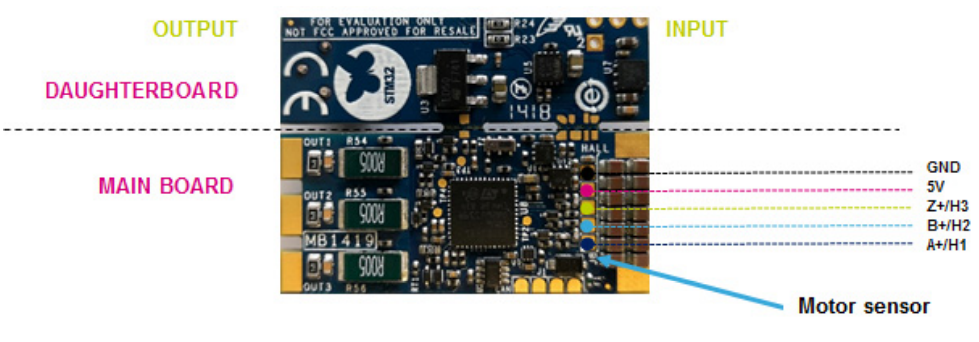
\includegraphics[width=\textwidth]{References/Sensor Wiring.png}}
                \caption{Board Sensor Wiring}
            \end{figure}
            \begin{figure}[H]
                \centerline{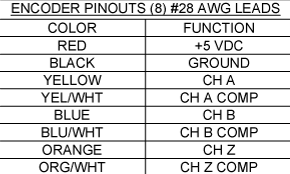
\includegraphics[width=\textwidth]{References/QEI Wiring.png}}
                \caption{Quadrature Encoder Wiring}
            \end{figure}
            \begin{figure}[H]
                \centerline{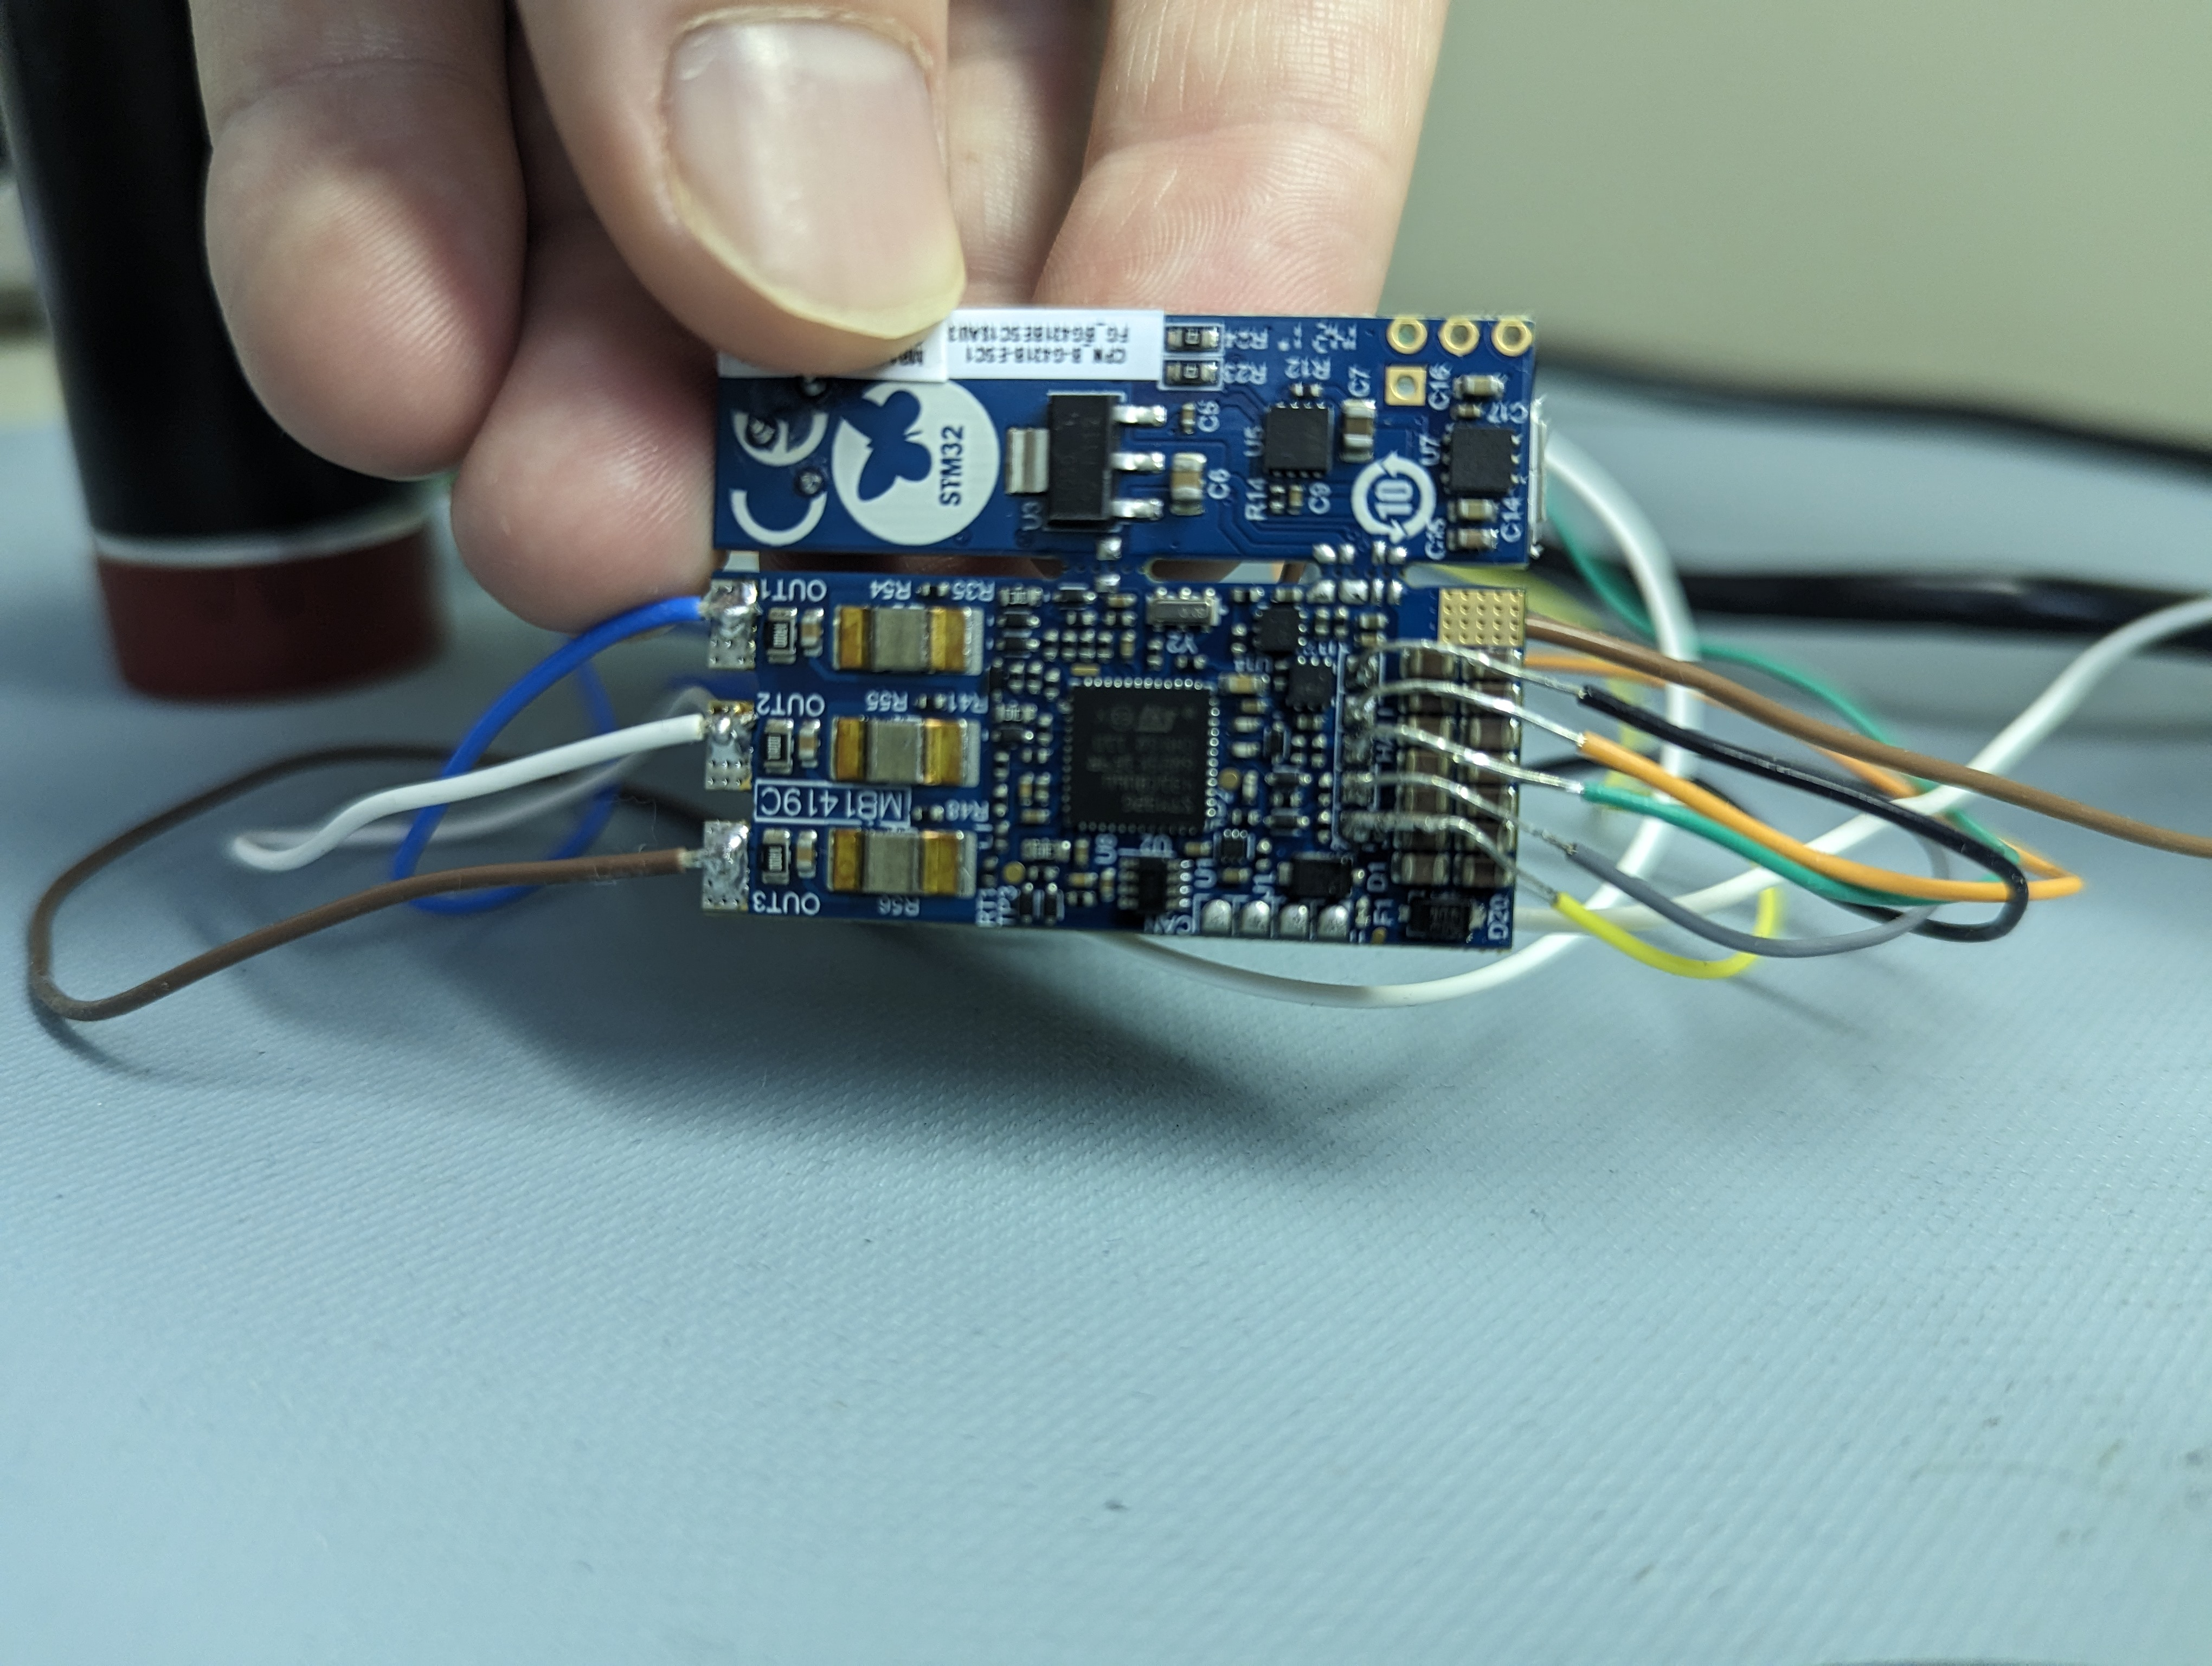
\includegraphics[width=\textwidth]{References/QEI Wiring Board Picture.jpg}}
                \caption{Quadrature Encoder Wiring Board Picture}
            \end{figure}
		\FloatBarrier \subsection{GIT Code}
            To make working in this document easier, my versions of the below examples will be included in a git repository that you can download. You do not need to complete this step, but it may be useful for comparing your project to a completed one. \\
            \textbf{Branch} - QEI-MotorControl
		\FloatBarrier \subsection{MotorControl Workbench}
            \textbf{Commit} - 60a5b83de6afa35f16d11d94896166aaf8240ad2 \\
            \begin{itemize}
                \item Open MotorControl Workbench (the latest version you have). 
                    \begin{figure}[H]
                        \centerline{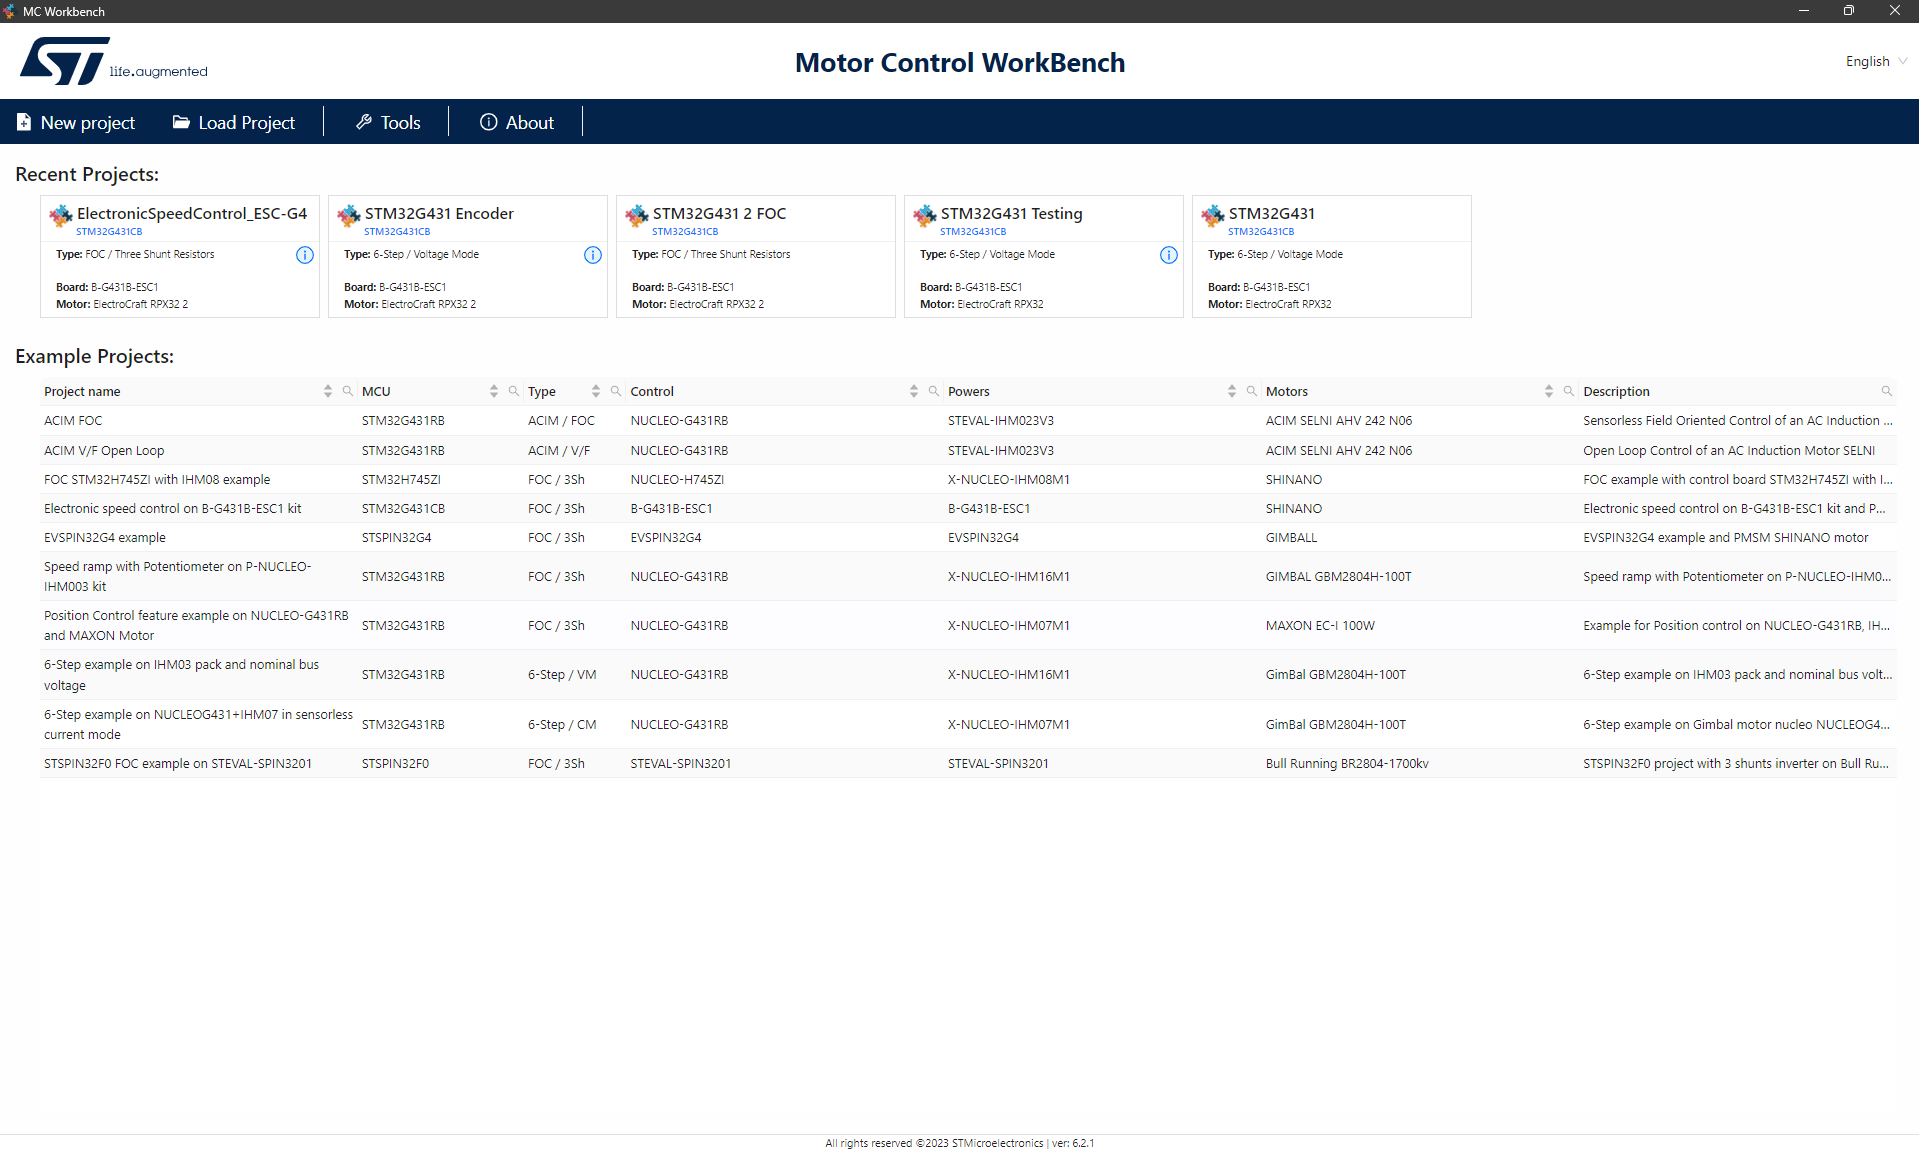
\includegraphics[width=\textwidth]{References/MC Workbench.png}}
                        \caption{MotorControl Workbench}
                    \end{figure}
                \item Select \emph{New project} in the top left.
                \item Give your project a name like "STM32G431 QEI Motor Control"
                \item \emph{Num. Motors} is 1 Motor, \emph{Driving Algorithm} is FOC, and \emph{Hardware Mode} is Inverter. Click Next at the bottom right.
                    \begin{figure}[H]
                        \centerline{\includegraphics[width=\textwidth]{References/MCW QEI New Project.png}}
                        \caption{MotorControl Workbench New Project}
                    \end{figure}
                \item Select the Motor you profiled in the previous section. Click Next
                \item Select B-G431B-ESC1 as your board. Click OK.
                \item This will bring you to the MotorControl Workbench Project screen.
                    \begin{figure}[H]
                        \centerline{\includegraphics[width=\textwidth]{References/MCW Project Screen.png}}
                        \caption{MotorControl Workbench Project Screen}
                    \end{figure}
                \item From here, either click on \emph{Motor} on the left hand side or click the motor on the right hand side. Scroll down on this page to where is says \emph{Quadrature Encoder} and turn this on and make sure \emph{Pulses per mechanical revolution} is set to 1024 and the \emph{Has index pin (Ch Z)} box is checked.
                    \begin{figure}[H]
                        \centerline{\includegraphics[width=\textwidth]{References/MCW FOC Quadrature Encoder.png}}
                        \caption{MotorControl Workbench Quadrature Encoder Select}
                    \end{figure}
                \item Select \emph{PWM Generation} and set \emph{PWM Frequency} to 40000 Hz.
                    \begin{figure}[H]
                        \centerline{\includegraphics[width=\textwidth]{References/MCW FOC PWM Gen.png}}
                        \caption{MotorControl Workbench PWM Generation Section}
                    \end{figure}
                \item Select \emph{Speed Sensing Selection} and select \emph{Quadrature Encoder} in \emph{Speed Sensor Mode}.
                    \begin{figure}[H]
                        \centerline{\includegraphics[width=\textwidth]{References/MCW FOC QEI Speed Sensing.png}}
                        \caption{MotorControl Workbench Speed Sensing Selection}
                    \end{figure}
                \item Finally, select \emph{Speed Sensing Config.} and set \emph{Final current ramp value} to 2 A and select \emph{OK} in the bottom right.
                    \begin{figure}[H]
                        \centerline{\includegraphics[width=\textwidth]{References/MCW FOC QEI Speed Sensing Config.png}}
                        \caption{MotorControl Workbench Speed Sensing Config}
                    \end{figure}
                \item Click \emph{Generate the project} at the top of the screen and save it.
                \item Next the \emph{Project generation} screen will appear. Select the latest version of STM32CubeMX as your \emph{STM32CubeMX} version, select \emph{IAR EWARM V8} as your \emph{Target Toolchain}, and leave the recommended firmware under \emph{Firmware Package Version} and \emph{HAL - Hardware Abstraction Layer} as \emph{Drive Type}.
                    \begin{figure}[H]
                        \centerline{\includegraphics[width=\textwidth]{References/MCW Project Gen.png}}
                        \caption{MotorControl Workbench Project Generation Screen}
                    \end{figure}
                \item Select \emph{GENERATE}. It may ask you to install firmware, do so if prompted.
                \item Once completed, select \emph{RUN STM32CubeMX}.
            \end{itemize}
		\FloatBarrier \subsection{STM32CubeMX}
            The only thing required to do in STM32CubeMX is click \emph{GENERATE CODE} in the top right and then \emph{Open Project} when completed. You may be tempted to skip this step is subsequent runs as MotorControl Workbench will automatically regenerate some code, but if anything involving the ports needs to be updated, STM32CubeMX will need to be run.
            \begin{figure}[H]
                \centerline{\includegraphics[width=\textwidth]{References/CubeMX.png}}
                \caption{STM32CubeMX Project Screen}
                    \end{figure}
		\FloatBarrier \subsection{IAR EW for ARM}
                    A screen will pop up asking if you would like to upgrade the project to the latest IAR version. Do so. You can compile and download the project to the board in IAR using the green button with a white triangle. You can turn on and off the motor using the button on the control board.
			\FloatBarrier \subsubsection{Motor Functions}
                        There are three main functions used in the operation of the motor in this section.
                        \begin{enumerate}
                            \item \texttt{MC\_StartMotor1(void)} - Starts the motor.
                            \item \texttt{MC\_StopMotor1(void)} - Stops the motor
                            \item \texttt{MC\_ProgramSpeedRampMotor1\_F(float\_t FinalSpeed, uint16\_t hDurationms)} - Select motor rotation speed. \texttt{FinalSpeed} is in RPM, the sign of this number is the rotation direction. \texttt{hDurationms} is number of milliseconds it will take the motor to reach this speed. 0 is follow mode which I have found to not be very accurate, the minimum I would set this is 20 ms.
                        \end{enumerate}
			\FloatBarrier \subsubsection{While Loop Motor Operation}
                \textbf{Commit} - e15a512e1b95627c5a91c302639088bd1ba0bd19 \\
                When code is generated by the MotorControl Workbench or STM32CubeMX, there will be \texttt{/* USER CODE */} around sections that will survive from one generation to the next. Additionally we can use the function \texttt{HAL\_Delay(delay\_ms)} to insert a delay between operations. Therefore the code 
                \begin{verbatim}
while (1)
{
    /* USER CODE END WHILE */

    /* USER CODE BEGIN 3 */
    MC_StartMotor1();
    HAL_Delay(2000);
    MC_StopMotor1();
    HAL_Delay(400);
}
                \end{verbatim}
                will start the motor, delay by 2000 ms (2 seconds), stop the motor, delay by 400 ms, then loop back to the top. \\ 
                You should always set a speed before stating the motor for the first time. In the section labeled \texttt{/* USER CODE BEGIN 2 */}, insert
                \begin{verbatim}
/* USER CODE BEGIN 2 */
MC_ProgramSpeedRampMotor1_F(1500, 1000);

/* USER CODE END 2 */
                \end{verbatim}
                 This will set the motor to 1500 RPM after a 1000 ms (1 second) ramp up period. You can now compile, download, and run this code on your board. You will need to hit the white circle with blue arrow in it at the top of IAR to run the code. You can mess around with the button and other functions like previous sections have done from here. 
	\FloatBarrier \section{Position Control}
    In order to use position control, it is required to use the quadrature encoder. Please make sure you have that section working before trying this section as position control is tricky and verifying that the motor is working correctly before is useful in identifying problems.
		\FloatBarrier \subsection{GIT Code}
            To make working in this document easier, my versions of the below examples will be included in a git repository that you can download. You do not need to complete this step, but it may be useful for comparing your project to a completed one. \\
            \textbf{Branch} - Position-MotorControl
		\FloatBarrier \subsection{MotorControl Workbench}
            \textbf{Commit} - f53a835f8103256d4e5a182d11f7705bddfe0720 \\
            This is where most of the difference between position control and previous projects occurs. There are a lot of parameters that need to be tuned correctly to get position control working accurately.
            \begin{itemize}
                \item Open MotorControl Workbench (the latest version you have). 
                    \begin{figure}[H]
                        \centerline{\includegraphics[width=\textwidth]{References/MC Workbench.png}}
                        \caption{MotorControl Workbench}
                    \end{figure}
                \item Select \emph{New project} in the top left.
                \item Give your project a name like "STM32G431 Position Motor Control"
                \item \emph{Num. Motors} is 1 Motor, \emph{Driving Algorithm} is FOC, and \emph{Hardware Mode} is Inverter. Click Next at the bottom right.
                    \begin{figure}[H]
                        \centerline{\includegraphics[width=\textwidth]{References/MCW Position New Project.png}}
                        \caption{MotorControl Workbench New Project}
                    \end{figure}
                \item Select the Motor you profiled in the previous section. Click Next
                \item Select B-G431B-ESC1 as your board. Click OK.
                \item This will bring you to the MotorControl Workbench Project screen.
                    \begin{figure}[H]
                        \centerline{\includegraphics[width=\textwidth]{References/MCW Project Screen.png}}
                        \caption{MotorControl Workbench Project Screen}
                    \end{figure}
                \item From here, either click on \emph{Motor} on the left hand side or click the motor on the right hand side. Scroll down on this page to where is says \emph{Quadrature Encoder} and turn this on and make sure \emph{Pulses per mechanical revolution} is set to 1024 and the \emph{Has index pin (Ch Z)} box is checked.
                    \begin{figure}[H]
                        \centerline{\includegraphics[width=\textwidth]{References/MCW FOC Quadrature Encoder.png}}
                        \caption{MotorControl Workbench Quadrature Encoder Select}
                    \end{figure}
                \item Leave \emph{PWM Frequency} alone for position control.
                \item Select \emph{Speed Sensing Config.} and check the \emph{Use absolute position control pin (ENC\_Z)} and set \emph{Duration} to 1000 ms and \emph{Final current ramp value} to 1A for now. We may need to tweak these later.
                    \begin{figure}[H]
                        \centerline{\includegraphics[width=\textwidth]{References/MCW Position Speed Sensing Config.png}}
                        \caption{MotorControl Workbench Speed Sensing Config}
                    \end{figure}
                \item Finally, select \emph{Drive Settings} and set \emph{Execution rate} to 0.5 ms. We may need to tweak this later. Select \emph{OK} in the bottom right.
                    \begin{figure}[H]
                        \centerline{\includegraphics[width=\textwidth]{References/MCW Position Drive Settings.png}}
                        \caption{MotorControl Workbench Drive Settings}
                    \end{figure}
                \item Click \emph{Generate the project} at the top of the screen and save it.
                \item Next the \emph{Project generation} screen will appear. Select the latest version of STM32CubeMX as your \emph{STM32CubeMX} version, select \emph{IAR EWARM V8} as your \emph{Target Toolchain}, and leave the recommended firmware under \emph{Firmware Package Version} and \emph{HAL - Hardware Abstraction Layer} as \emph{Drive Type}.
                    \begin{figure}[H]
                        \centerline{\includegraphics[width=\textwidth]{References/MCW Project Gen.png}}
                        \caption{MotorControl Workbench Project Generation Screen}
                    \end{figure}
                \item Select \emph{GENERATE}. It may ask you to install firmware, do so if prompted.
                \item Once completed, select \emph{RUN STM32CubeMX}.
            \end{itemize}
		\FloatBarrier \subsection{STM32CubeMX}
            The only thing required to do in STM32CubeMX is click \emph{GENERATE CODE} in the top right and then \emph{Open Project} when completed. You may be tempted to skip this step is subsequent runs as MotorControl Workbench will automatically regenerate some code, but if anything involving the ports needs to be updated, STM32CubeMX will need to be run.
            \begin{figure}[H]
                \centerline{\includegraphics[width=\textwidth]{References/CubeMX.png}}
                \caption{STM32CubeMX Project Screen}
                    \end{figure}
		\FloatBarrier \subsection{IAR EW for ARM}
            A screen will pop up asking if you would like to upgrade the project to the latest IAR version. Do so. You can compile and download the project to the board in IAR using the green button with a white triangle. You can turn on and off the motor using the button on the control board. Before we do anything however, we should open up \emph{Motor Pilot 6.2.1}.
            \begin{figure}[H]
                \centerline{\includegraphics[width=\textwidth]{References/Motor Pilot Position Control.png}}
                \caption{Motor Pilot Position Control}
            \end{figure}
            This will look different than previous sections as it is displaying and targeting position.
			\FloatBarrier \subsubsection{Motor Functions}
                There are quite a few new functions to learn for position control.
                \begin{enumerate}
                    \item \texttt{void MC\_StartMotor1(void)} - Starts the motor.
                    \item \texttt{void MC\_StopMotor1(void)} - Stops the motor
                    \item \texttt{void MC\_ProgramPositionCommandMotor1(float\_t fTargetPosition, float\_t fDuration)} - Select motor rotation position. \texttt{fTargetPosition} is in radians, it is the position you want to the motor to go to with the sign of this number begin the rotation direction. \texttt{hDurationms} is number of milliseconds it will take the motor to reach this position. 0 is follow mode which I have found to not be very accurate, the minimum I would set this is 20 ms.
                    \item \texttt{AlignStatus\_t MC\_GetAlignmentStatusMotor1(void)} - Alignment state of the motor. \emph{AlignStatus\_t} returns the status of the alignment, whether it was successful or not. 
                    \item \texttt{float\_t MC\_GetCurrentPosition1(void)} - Current position for the motor. It returns the current position of the motor in radians.
                    \item \texttt{float\_t MC\_GetTargetPosition1(void)} - Target position for the motor. It returns the target position of the motor in radians.
                \end{enumerate}
			\FloatBarrier \subsubsection{Default Motor Position Operation}
                \textbf{Commit} - f3f8bed7811cb81cf51ac2909cdddcb9db227fae \\
                The document \href{https://www.st.com/resource/en/application_note/dm00691525-position-control-of-a-threephase-permanent-magnet-motor-using-xcubemcsdk-or-xcubemcsdkful-stmicroelectronics.pdf}{Position control of a three-phase permanent magnet motor using X‑CUBE‑MCSDK or X‑CUBE‑MCSDK-FUL} describes getting basic position control with the motor working, including section 5 which lays out a default program shown below.
                \begin{verbatim}
/* USER CODE BEGIN 2 */
MC_StartMotor1();
/* USER CODE END 2 */
/* Infinite loop */
/* USER CODE BEGIN WHILE */
while(MC_GetAlignmentStatusMotor1()!=TC_ALIGNMENT_COMPLETED){}
while (1)
{
 /* USER CODE END WHILE */
 /* USER CODE BEGIN 3 */
 MC_ProgramPositionCommandMotor1(3.14/2,0.1);
 HAL_Delay(2000);
 MC_ProgramPositionCommandMotor1(-3.14/2,0.1);
 HAL_Delay(2000);
}
/* USER CODE END 3 */
                \end{verbatim}
                This code goes in the main loop of the program towards the end. Step by step 
                \begin{enumerate}
                    \item \texttt{MC\_StartMotor1();} starts the motor.
                    \item \texttt{while(MC\_GetAlignmentStatusMotor1()!=TC\_ALIGNMENT\_COMPLETED){}} waits for the motor be finish alignment.
                    \item \texttt{MC\_ProgramPositionCommandMotor1(3.14/2,0.1);} rotates the motor to pi/2 radians with \texttt{MC\_ProgramPositionCommandMotor1(-3.14/2,0.1);} rotating it to -pi/2 radians.
                \end{enumerate}
                Pull up the Motor Pilot and run this code to verify that your position control algorithm is working. If not, you probably need to increase \emph{Final current ramp value} if you get an error or \emph{Execution rate} if the motor is swinging wildly. The motor pilot should show you the current position of the motor and if any faults have occurred. If faults have occurred, acknowledged them and try starting the motor again.
			\FloatBarrier \subsubsection{Other Motor Position Operation}
                \textbf{Commit} - 31796d744b39cee1fbfd82b385be8d45bd90c2a1 \\
                It is important that your delays are at least as long as the time it takes to rotate, otherwise the rotation will not complete. We can rotate the motor as far in either direction as we wish, the below example will rotate it slowly to positive 10pi and then slowly to negative 10pi. This replaces the \texttt{while(1)} loop.
                \begin{verbatim}
/* USER CODE BEGIN 2 */
const float_t PI                = 3.14;
const float_t POS_INCR          = PI / 4.0f;
const float_t NEG_INCR          = PI / -4.0f;
const float_t POS_POSITION_END  = 10.0f*PI;
const float_t NEG_POSITION_END  = -10.0f*PI;
const float_t DURATION_S        = 1.0f;
const int16_t DELAY_MS          = 2000; // DELAY_MS >= 1000*DURATION_S

float_t position = 0;

MC_StartMotor1();
/* USER CODE END 2 */
/* Infinite loop */
/* USER CODE BEGIN WHILE */
while(MC_GetAlignmentStatusMotor1()!=TC_ALIGNMENT_COMPLETED){}
while (position < POS_POSITION_END)
{
 /* USER CODE END WHILE */
 /* USER CODE BEGIN 3 */
    position += POS_INCR;
    MC_ProgramPositionCommandMotor1(position,DURATION_S);
    HAL_Delay(DELAY_MS);
}
while (position > NEG_POSITION_END)
{
    position += NEG_INCR; // NEG_INCR already negative
    MC_ProgramPositionCommandMotor1(position,DURATION_S);
    HAL_Delay(DELAY_MS);
}
/* USER CODE END 3 */
                \end{verbatim}
			\FloatBarrier \subsubsection{Motor Position Playground}
                \textbf{Commit} - 6fd87411d23abcac93e83c9ca5c847d6db8deaf8 \\
                This section commit is where I have dumped my work for getting the motor operational. There are several new operations of this commit, namely getting the actual motor control handler in main, saving off and restoring the position to a file, automatic restart of alignment if it fails, and using the \texttt{MC\_GetCurrentPosition1()} to get the position of the motor. There are also several other functions in this commit that help with gathering information about the motor. Below is a list of lessons I have learned along the way. Please note that rerunning \emph{MotorControl Workbench} will overwrite some of these changes. 
                \begin{enumerate}
                    \item The movement duration should be at least 20 ms (\texttt{DURATION\_S = 0.02f}).
                    \item The timer attached to the motor control handler has a \emph{CNT} variable which gives you the direction that the stator is facing, relative to where the motor started at power on. This can be useful for trying to figure out exactly where the motor is facing. 
                    \item The max deviation I have seen of the timer CNT from the position returned by \texttt{MC\_GetCurrentPosition1()} is around 21 degrees. From this, we are still able to tell where we should be (need to be within 22.5 degrees) but is worrying. However, usually in my runs the max is around 7.5 degrees, which is pretty manageable.
                    \item An alignment failing is due to either the startup current being too low (1 A works) or the Voltage multiplier being to low (16 times works).
                    \item I still need to try to figure out why alignment fails due to over current.
                \end{enumerate}
	\FloatBarrier \section{Miscellaneous Projects}
    This section is working on other projects dealing with the board and the motor. So far, controlling the LED and potentiometer on the board have been added.
		\FloatBarrier \subsection{GIT Code}
            To make working in this document easier, my versions of the below examples will be included in a git repository that you can download. You do not need to complete this step, but it may be useful for comparing your project to a completed one. \\
            \textbf{Branch} - Miscellaneous-MotorControl
		\FloatBarrier \subsection{MotorControl Workbench}
            \textbf{Commit} - fb54b93c5a6bb1ff13d5c1ef8d73b0d5a788a664 \\
            This section shows you have to initialize the potentiometer. This is as simple as checking the \emph{Potentiometer} checkbox as shown below. One note is that you cannot use a potentiometer with sensorless motor control.
            \begin{itemize}
                \item Open MotorControl Workbench (the latest version you have). 
                    \begin{figure}[H]
                        \centerline{\includegraphics[width=\textwidth]{References/MC Workbench.png}}
                        \caption{MotorControl Workbench}
                    \end{figure}
                \item Select \emph{New project} in the top left.
                \item Give your project a name like "STM32G431 Miscellaneous Motor Control"
                \item \emph{Num. Motors} is 1 Motor, \emph{Driving Algorithm} is FOC, and \emph{Hardware Mode} is Inverter. Click Next at the bottom right.
                    \begin{figure}[H]
                        \centerline{\includegraphics[width=\textwidth]{References/MCW Miscellaneous New Project.png}}
                        \caption{MotorControl Workbench New Project}
                    \end{figure}
                \item Select the Motor you profiled in the previous section. Click Next
                \item Select B-G431B-ESC1 as your board. Click OK.
                \item This will bring you to the MotorControl Workbench Project screen. 
                    \begin{figure}[H]
                        \centerline{\includegraphics[width=\textwidth]{References/MCW Project Screen.png}}
                        \caption{MotorControl Workbench Project Screen}
                    \end{figure}
                \item From here, either click on \emph{Motor} on the left hand side or click the motor on the right hand side. Scroll down on this page and enter the parameters of the sensor you have hooked up (120 for Hall-Effect, 1024 for Quadrature Encoder).
                    \begin{figure}[H]
                        \centerline{\includegraphics[width=\textwidth]{References/MCW 6-step Hall-Effect Motor.png}}
                        \caption{MotorControl Workbench Hall-Effect Select}
                    \end{figure}
                \item Select \emph{Speed Sensing Selection} and select \emph{Hall-Effect} or \emph{Quadrature Encoder} in \emph{Speed Sensor Mode}.
                    \begin{figure}[H]
                        \centerline{\includegraphics[width=\textwidth]{References/MCW FOC Speed Sensing Selection.png}}
                        \caption{MotorControl Workbench Speed Sensing Selection}
                    \end{figure}
                \item click on \emph{Stage Configuration} on the left hand side. Turn on the \emph{Potentiometer} toggle. Select \emph{OK} in the bottom right.
                    \begin{figure}[H]
                        \centerline{\includegraphics[width=\textwidth]{References/MCW 6-step Potentiometer.png}}
                        \caption{MotorControl Workbench Potentiometer Select}
                    \end{figure}
                \item Click \emph{Generate the project} at the top of the screen and save it.
                    \begin{figure}[H]
                        \centerline{\includegraphics[width=\textwidth]{References/MCW Project Screen.png}}
                        \caption{MotorControl Workbench Project Screen}
                    \end{figure}
                \item Next the \emph{Project generation} screen will appear. Select the latest version of STM32CubeMX as your \emph{STM32CubeMX} version, select \emph{IAR EWARM V8} as your \emph{Target Toolchain}, and leave the recommended firmware under \emph{Firmware Package Version} and \emph{HAL - Hardware Abstraction Layer} as \emph{Drive Type}.
                    \begin{figure}[H]
                        \centerline{\includegraphics[width=\textwidth]{References/MCW Project Gen.png}}
                        \caption{MotorControl Workbench Project Generation Screen}
                    \end{figure}
                \item Select \emph{GENERATE}. It may ask you to install firmware, do so if prompted.
                \item Once completed, select \emph{RUN STM32CubeMX}.
            \end{itemize}
		\FloatBarrier \subsection{STM32CubeMX}
            For the first time, we will be doing something in STM32CubeMX. As you probably noticed, when you launch this program, the pinout of your chip will appear on the screen. 
            \begin{figure}[H]
                \centerline{\includegraphics[width=\textwidth]{References/CubeMX.png}}
                \caption{STM32CubeMX Project Screen}
            \end{figure}
            The LED is associated with \emph{PC6}. Click on this pin on the screen (it is on the bottom right of the chip and select \emph{GPIO Output}. 
            \begin{figure}[H]
                \centerline{\includegraphics[width=\textwidth]{References/CubeMX PC6 GPIO Out.png}}
                \caption{STM32CubeMX GPIO PC6 Output Select}
            \end{figure}
            After this, the only thing required to do in STM32CubeMX is click \emph{GENERATE CODE} in the top right and then \emph{Open Project} when completed. You may be tempted to skip this step is subsequent runs as MotorControl Workbench will automatically regenerate some code, but if anything involving the ports needs to be updated, STM32CubeMX will need to be run.
		\FloatBarrier \subsection{IAR EW for ARM}
            A screen will pop up asking if you would like to upgrade the project to the latest IAR version. Do so. You can compile and download the project to the board in IAR using the green button with a white triangle. You can turn on and off the motor using the button on the control board.
			\FloatBarrier \subsubsection{Motor Functions}
                There are two main functions used in the operation of the motor in this section. You cannot control the speed with the \texttt{MC\_ProgramSpeedRampMotor1\_F} function while using the potentiometer.
                \begin{enumerate}
                    \item \texttt{MC\_StartMotor1(void)} - Starts the motor.
                    \item \texttt{MC\_StopMotor1(void)} - Stops the motor
                \end{enumerate}
			\FloatBarrier \subsubsection{Potentiometer Operation}
            Out of the box, the potentiometer will function properly. You can use the default button implementation of the motor and twist the potentiometer to change the speed of the motor. You can compile, download, and run this code on your board. You will need to hit the white circle with blue arrow in it at the top of IAR to run the code.
			\FloatBarrier \subsubsection{Button LED Operation}
            \textbf{Commit} - a28700f1779e3e01ad4750c616e1a2f7e5598f09 \\ 
            The function \texttt{void HAL\_GPIO\_WritePin(GPIO\_TypeDef *GPIOx, uint16\_t GPIO\_Pin, GPIO\_PinState PinState)} changes the output of the a given GPIO pin. You can turn the LED off with \texttt{HAL\_GPIO\_WritePin(GPIOC, GPIO\_PIN\_6, GPIO\_PIN\_RESET)} and on with \texttt{HAL\_GPIO\_WritePin(GPIOC, GPIO\_PIN\_6, GPIO\_PIN\_SET)}. We can leverage the button function \texttt{UI\_HandleStartStopButton\_cb} to turn on and off the LED with with the motor.
            \begin{verbatim}
__weak void UI_HandleStartStopButton_cb (void)
{
/* USER CODE BEGIN START_STOP_BTN */
  if (IDLE == MC_GetSTMStateMotor1())
  {
    /* Ramp parameters should be tuned for the actual motor */
    (void)MC_StartMotor1();
    HAL_GPIO_WritePin(GPIOC, GPIO_PIN_6, GPIO_PIN_SET);
  }
  else
  {
    (void)MC_StopMotor1();
    HAL_GPIO_WritePin(GPIOC, GPIO_PIN_6, GPIO_PIN_RESET);
  }
/* USER CODE END START_STOP_BTN */
}
            \end{verbatim}
            Build, run, and test this code. This will now turn on and off the LED with the button, with the potentiometer controlling the speed.         
\end{document}